\newcommand{\defs}{../defs}
\documentclass[12pt]{scrbook}

\usepackage{\defs/tikz-uml}

\usepackage[T1]{fontenc}
\usepackage[utf8x]{inputenc}
\usepackage{lmodern}
\usepackage[brazilian]{babel}
\usepackage{minted}
\usepackage[a4paper, margin=1in, footskip=0.5in]{geometry}
\usepackage{url}
\usepackage{graphicx}
\usepackage[export]{adjustbox}
\usepackage{hyperref}
\usepackage[square]{natbib}
\usepackage[parfill]{parskip}
\usepackage{mdframed}
\usepackage{longtable}
\usepackage{soul}
\usepackage{tabularx}
\usepackage[shortlabels]{enumitem}
\usepackage{xifthen}
\usepackage{multirow}

\hypersetup{
	colorlinks,
	linkcolor={blue!80!black},
	citecolor={blue!80!black},
	urlcolor={blue!80!black}
}

\definecolor{codelinecolor}{gray}{.90}
%\definecolor{codelinecolor}{gray}{.85}%print version
\colorlet{codeboxcolor}{green!10}
%\colorlet{codeboxcolor}{gray!30}%print version
\sethlcolor{codelinecolor}

\newcommand{\modulo}{{\color{gray}\%}}

\usepackage[automark,headsepline,footsepline]{scrlayer-scrpage}
\lehead{\myname}
\lohead{\myname}
\rehead{{\leftmark}}
\rohead{{\leftmark}}
\lefoot{}
\lofoot{}
\refoot{}
\rofoot{}
\cofoot{\\\thepage}
\cefoot{\\\thepage}
\setkomafont{pagehead}{\normalfont\small}
\setkomafont{pagefoot}{\normalfont}
\renewcommand{\chapterpagestyle}{scrheadings}

\title{\mytitle}

\author{\myname}
\publishers{%
	\logo%
	\university\\%
	\campus%
}

\date{}
\subject{}
\subtitle{}

\uppertitleback{
	\version \\ \\
	\presentation
}

\lowertitleback{\license}

\surroundwithmdframed{minted}

\BeforeBeginEnvironment{mdframed}{\bigskip}
\AfterEndEnvironment{mdframed}{\medskip}

\mdfsetup{%
	backgroundcolor=codeboxcolor,
	linecolor=white}

\setminted{%
	mathescape,
	linenos,
	breaklines,
	tabsize=3}

\newcommand{\code}[1]{%
	\texttt{\hl{#1}}%
}

\newcommand{\javacode}[1]{%
	\mintinline[escapeinside=~~]{java}{#1}
}

\newcommand{\javacodecolor}[1]{%
	\mintinline[escapeinside=~~,bgcolor=codeboxcolor]{java}{#1}
}

\tikzumlset{fill class=red!7}
\tikzumlset{font=\footnotesize}

\newcounter{number}[section]
\newenvironment{exercise}[1][]
{%
	\refstepcounter{number}%
	\noindent%
	\ifthenelse{\equal{\thesection}{0}}%
	{%
		\ifthenelse{\equal{#1}{}}%
		{\textbf{\exercisedescription~\thenumber.\\}}%
		{\textbf{\exercisedescription~\thenumber. (#1)\\}}%
	}%
	{%
		\ifthenelse{\equal{#1}{}}%
		{\textbf{\exercisedescription~\thesection.\thenumber.\\}}%
		{\textbf{\exercisedescription~\thesection.\thenumber. (#1)\\}}%
	}%
	\rmfamily%
}{\medskip}%

\makeatletter%
\setlength{\@fptop}{5pt}

\makeatletter
\DeclareOldFontCommand{\rm}{\normalfont\rmfamily}{\mathrm}
\DeclareOldFontCommand{\sf}{\normalfont\sffamily}{\mathsf}
\DeclareOldFontCommand{\tt}{\normalfont\ttfamily}{\mathtt}
\DeclareOldFontCommand{\bf}{\normalfont\bfseries}{\mathbf}
\DeclareOldFontCommand{\it}{\normalfont\itshape}{\mathit}
\DeclareOldFontCommand{\sl}{\normalfont\slshape}{\@nomath\sl}
\DeclareOldFontCommand{\sc}{\normalfont\scshape}{\@nomath\sc}
\makeatother

\newcommand{\myname}{Prof. Marcelo de Souza}
\newcommand{\university}{Universidade do Estado de Santa Catarina}
\newcommand{\campus}{Centro de Educação Superior do Alto Vale do Itajaí}
\newcommand{\mytitle}{Programação Orientada a Objetos\\Notas de Aula}
\newcommand{\version}{Versão compilada em \today.}
\newcommand{\exercisedescription}{Exercício}

\newcommand{\presentation}{Este material é utilizado em parte das aulas da disciplina de Programação I (25PRO1) do curso de Bacharelado em Engenharia de Software da Universidade do Estado de Santa Catarina (UDESC Ibirama).\\ \\
\textbf{Contato:} \texttt{marcelo.desouza@udesc.br}}

\newcommand{\license}{\small Esta obra está disponível sob uma Licença \href{https://creativecommons.org/licenses/by-nc-nd/4.0}{Creative Commons (BY-NC-ND 4.0 Internacional)}.}

\newcommand{\logo}{
\begin{figure}[h]
	\centering
	
\includegraphics[width=0.35\textwidth]{\defs/img/logo-udesc.png}
\end{figure}
}

\begin{document}

\maketitle
\tableofcontents

\part{Conceitos básicos}
\chapter{Linguagem Java}

\section{Variáveis e constantes}
Uma variável é um mapeamento para um espaço alocado de memória, no qual se pode armazenar valores de um determinado tipo. O exemplo abaixo mostra a declaração de variáveis, atribuição de valores e sua recuperação.

\begin{minted}{java}
int idade;                  //Declaração
idade = 10;                 //Atribuição
int valor = idade;          //Recuperação
System.out.println(idade);  //Recuperação e apresentação
\end{minted}

Uma constante nada mais é do que uma variável que possui um valor predeterminado, com alteração não permitida. O trecho de código abaixo exemplifica a declaração de uma constante (com seu valor fixo) e a recuperação deste valor. A criação de uma constante é feita pelo uso da palavra reservada \code{final}, que torna seu valor fixo e não permite alteração (valor final).

\begin{minted}{java}
final int matricula = 512010681;  //Declaração e atribuição
int aluno = matricula;            //Recuperação
System.out.println(matricula);    //Recuperação
\end{minted}

\section{Tipos primitivos em Java}

Existem quatro categorias básicas para variáveis em Java: numérico (armazenamento de números), caracter (armazenamento de caracteres), alfanumérico (armazenamento de valores textuais) e lógico (armazenamento de valores lógicos -- verdadeiro e falso). A Tabela~\ref{tab:tipos-primitivos} resume os tipos primitivos em Java para cada categoria e o tamanho ocupado em memória por variáveis de cada tipo.

\begin{table}[ht]
	\centering
	\begin{tabular}{llr}
		\hline
		\textbf{Categoria}    & \textbf{Tipo}    & \textbf{Tamanho} \\ \hline
		numérica     & byte   & 8 bits \\
		numérica     & short   & 16 bits \\
		numérica     & int     & 32 bits \\
		numérica     & long    & 64 bits \\
		numérica     & float   & 32 bits \\
		numérica     & double  & 64 bits \\
		alfanumética & char    & 16 bits \\
		lógica       & boolena & 1 bit \\\hline
	\end{tabular}
	\caption{Tipos primitivos em Java}
	\label{tab:tipos-primitivos}
\end{table}

O trecho de código abaixo mostra o uso de variáveis dos diferentes tipos, com o armazenamento de valores e a recuperação para apresentação em tela.

\begin{minted}{java}
String nome = "João";
int idade = 15;
char sexo = 'M';
boolean aprovado = true;
System.out.println("Dados do acadêmico"
                 + "\nNome: " + nome
                 + "\nIdade: " + idade
                 + "\nSexo: " + sexo
                 + "\nAprovado: " + aprovado);
\end{minted}

\section{Leitura de valores do usuário}

A classe \code{Scanner} pode ser utilizada para a leitura de valores a partir do console. Esta classe memoriza o valor digitado pelo usuário e armazena em uma variável indicada. O exemplo abaixo mostra a criação de um objeto (\code{scanner}) desta classe e a posterior leitura de valores.


\begin{minted}{java}
Scanner scanner = new Scanner(System.in);
int valorInteiro = scanner.nextInt();
String valorTextual = scanner.next();
double d = scanner.nextDouble();
\end{minted}

Uma alternativa ao uso do console como entrada e saída de dados consiste em apresentar ao usuário uma caixa de diálogo com as informações de saída ou com a solicitação de uma entrada. A classe \code{JOptionPane} fornece os métodos necessários a esta tarefa. O método \code{showMessageDialog} permite a apresentação de uma mensagem ao usuário, enquanto o método \code{showInputDialog} permite solicitar um valor ao usuário. Note que o método retorna um valor do tipo \code{String}, que deve ser convertido ao tipo desejado, caso diferente. O exemplo abaixo mostra o uso da classe \code{JOptionPane} para as tarefas supracitadas.

\begin{minted}{java}
JOptionPane.showMessageDialog(null, "Mensagem ao usuário");
int valorInteiro = Integer.parseInt(JOptionPane.showInputDialog("Digite um valor inteiro:"));
String valorTextual = JOptionPane.showInputDialog("Digite uma String:");
double d = Double.parseDouble(JOptionPane.showInputDialog("Digite um valor double: "));
\end{minted}


\section{Operadores aritméticos}

Operadores aritméticos são funções e operadores predefinidos para realização de cálculos matemáticos. Eles atuam sobre valores ou variáveis numéricas. A Tabela~\ref{tab:operadores-aritmeticos} apresenta os principais operadores aritméticos disponíveis na linguagem Java, seus exemplos e sua descrição.

\begin{table}[H]
	\centering
	\begin{tabular}{c|c|l}
		\hline
		\textbf{Operador} & \textbf{Exemplo} & \textbf{Descrição}\\ \hline
		\texttt{=}   	 & \texttt{x = y}	   & O conteúdo da variável \texttt{y} é atribuído à variável \texttt{x}.  \\
		\texttt{+} 		 & \texttt{x + y}     & Soma o conteúdo de \texttt{x} e de \texttt{y}.\\
		\texttt{-}  		 & \texttt{x - y}     & Subtrai o conteúdo de \texttt{y} do conteúdo de \texttt{x}.\\
		\texttt{*}  		 & \texttt{x * y}     & Multiplicação conteúdo de \texttt{x} com o conteúdo de \texttt{y}.\\
		\texttt{/}  		 & \texttt{x / y}     & Divide o conteúdo de \texttt{x} pelo conteúdo de \texttt{y}.\\
		\texttt{\%} 		 & \texttt{x \% y} & Obtém o resto da divisão inteira de \texttt{x} por \texttt{y}.\\
		\texttt{++}  	 & \texttt{x++}     & Equivale a \texttt{x = x + 1}.\\
		\texttt{----}  	 & \texttt{x----}     & Equivale a \texttt{x = x - 1}.\\ \hline                           
	\end{tabular}
	\caption{Operadores Aritméticos}
	\label{tab:operadores-aritmeticos}
\end{table}

O trecho de código abaixo exemplifica a aplicação dos operadores supracitados. Em expressões mais complexas, os operadores têm a mesma precedência que na matemática básica, a qual pode ser alterada com o uso de parêntesis.

\begin{minted}{java}
int a, b, resultado;
a = 10;
b = 3;
resultado = a + b;         //resultado -> 13
resultado = a - b;         //resultado -> 7
resultado = a * b;         //resultado -> 30
resultado = a / b;         //resultado -> 3
resultado = (a / b) + a ;  //resultado -> 13
resultado = a % b;         //resultado -> 1
resultado = a++;           //resultado -> ???
resultado = b--;           //resultado -> ???
\end{minted}

O resultado das expressões apresentadas nas linhas 10 e 11 é \code{10} e \code{3}, respectivamente. Isto se deve ao fato de que as operações \code{a++} e \code{b--} são realizadas após a atribuição, ou seja, após os valores originais serem armazenados na variável \code{resultado}. Para que as operações sobre as variáveis \code{a} e \code{b} sejam feitas antes da atribuição, deve-se utilizar \code{++a} e \code{++b}.

\section{Operadores lógicos}
Operadores lógicos são funções ou operadores predefinidos para atuação sobre valores ou variáveis booleanas (lógicas), avaliando seu conteúdo. Estes operadores retornam um valor booleano (\code{true} ou \code{false}) como resultado. A Tabela~\ref{tab:operadores-logicos} apresenta uma visão geral dos operadores lógicos (\texttt{AND}, \texttt{OR} e \texttt{NOT}). As Tabelas~~\ref{tab:operador-e},~\ref{tab:operador-ou} e~\ref{tab:operador-not} detalham o funcionamento de cada operador, apresentando a tabela verdade de cada um.

\begin{table}[H]
	\centering
	\begin{tabular}{l|c|l}
		\hline
		\textbf{Operador}       & \textbf{Exemplo}  & \textbf{Descrição}                               \\ \hline
		E/AND -- \texttt{\&\&} & \texttt{x \&\& y} & Representa o conteúdo de \texttt{x} \textbf{E} o conteúdo de \texttt{y}  \\
		
		OU/OR -- \texttt{||}   & \texttt{x || y}   & Representa o conteúdo de \texttt{x} \textbf{OU} o conteúdo de \texttt{y} \\
		
		NÃO/NOT -- \texttt{!}  & \texttt{!x}       & Representa o valor inverso de \texttt{x} (não \texttt{x}). \\ \hline
	\end{tabular}
	\caption{Visão geral dos operadores lógicos}
	\label{tab:operadores-logicos}
\end{table}

\begin{table}[H]
	\centering
	\begin{tabular}{c|c|c|c}
		\hline
		\textbf{Valor de \texttt{x}} & \textbf{Operador} & \textbf{Valor de \texttt{y}} & \textbf{Resultado} \\ \hline
		\texttt{\color{green!50!black}TRUE}       & \texttt{\&\&}     & \texttt{\color{green!50!black}TRUE}       & \texttt{\color{green!50!black}TRUE}      \\
		\texttt{\color{green!50!black}TRUE}       & \texttt{\&\&}     & \texttt{\color{red!50!black}FALSE}      & \texttt{\color{red!50!black}FALSE}     \\
		\texttt{\color{red!50!black}FALSE}      & \texttt{\&\&}     & \texttt{\color{green!50!black}TRUE}       & \texttt{\color{red!50!black}FALSE}     \\
		\texttt{\color{red!50!black}FALSE}      & \texttt{\&\&}     & \texttt{\color{red!50!black}FALSE}      & \texttt{\color{red!50!black}FALSE}     \\ \hline
	\end{tabular}
	\caption{Tabela verdade para o operador \texttt{AND}}
	\label{tab:operador-e}	
\end{table}

\begin{table}[H]
	\centering
	\begin{tabular}{c|c|c|c}
		\hline
		\textbf{Valor de \texttt{x}} & \textbf{Operador} & \textbf{Valor de \texttt{y}} & \textbf{Resultado} \\ \hline
		\texttt{\color{green!50!black}TRUE}       & \texttt{||}       & \texttt{\color{green!50!black}TRUE}       & \texttt{\color{green!50!black}TRUE}      \\
		\texttt{\color{green!50!black}TRUE}       & \texttt{||}       & \texttt{\color{red!50!black}FALSE}      & \texttt{\color{green!50!black}TRUE}      \\
		\texttt{\color{red!50!black}FALSE}      & \texttt{||}       & \texttt{\color{green!50!black}TRUE}       & \texttt{\color{green!50!black}TRUE}      \\
		\texttt{\color{red!50!black}FALSE}      & \texttt{||}       & \texttt{\color{red!50!black}FALSE}      & \texttt{\color{red!50!black}FALSE}     \\ \hline
	\end{tabular}
	\caption{Tabela verdade para o operador \texttt{OR}}
	\label{tab:operador-ou}	
\end{table}

\begin{table}[H]
	\centering
	\begin{tabular}{c|c|c}
		\hline
		\textbf{Operador} & \textbf{Valor de \texttt{x}} & \textbf{Resultado} \\ \hline
		\texttt{!}        & \texttt{\color{green!50!black}TRUE}       & \texttt{\color{red!50!black}FALSE}     \\
		\texttt{!}        & \texttt{\color{red!50!black}FALSE}      & \texttt{\color{green!50!black}TRUE}      \\ \hline
	\end{tabular}
	\caption{Tabela verdade para o operador \texttt{NOT}}
	\label{tab:operador-not}
\end{table}

O trecho de código a seguir mostra a aplicação dos operadores lógicos sobre variáveis booleanas.

\begin{minted}{java}
boolean a, b, resultado;
a = true;
b = false;
resultado = a && b;  //resultado -> false
resultado = a || b;  //resultado -> true
resultado = !a;      //resultado -> false
\end{minted}

\section{Operadores relacionais}
Operadores relacionais são funções ou operadores predefinidos para atuação sobre valores ou variáveis de diferentes tipos, comumente numéricos. Estes operadores avaliam o conteúdo de duas variáveis ou grandezas e os compara, retornando um valor lógico (\code{true} ou \code{false}). Em outras palavras, estes operadores relacionam duas variáveis ou duas grandezas, comparando-as.

\begin{table}[H]
	\centering
	\begin{tabular}{l|c|l}
		\hline
		\textbf{Operador}       & \textbf{Exemplo}                              & \textbf{Descrição}                                       \\ \hline
		Igual -- \texttt{==}          &       \texttt{x==y}                        & Conteúdo de \texttt{x} é igual ao conteúdo de \texttt{y}?          \\
		Diferente -- \texttt{!=}      &         \texttt{x!=y}                       & Conteúdo de \texttt{x} é diferente do conteúdo de \texttt{y}?      \\
		Maior -- \texttt{>}          & \texttt{x > y} 			  & Conteúdo de \texttt{x} é maior que o conteúdo de \texttt{y}?       \\
		Menor -- \texttt{<}          & \texttt{x < y}       		  & Conteúdo de \texttt{x} é menor que o conteúdo de \texttt{y}?       \\
		Maior ou igual -- \texttt{>=} & \texttt{x >= y} & Conteúdo de \texttt{x} é maior ou igual ao conteúdo de \texttt{y}? \\
		Menor ou igual -- \texttt{<=} & \texttt{x <= y}       & Conteúdo de \texttt{x} é menor ou igual ao conteúdo de \texttt{y}? \\ \hline
	\end{tabular}
	\caption{Operadores relacionais}
\end{table}

O trecho de código a seguir mostra a aplicação dos diferentes operadores relacionais, avaliando o conteúdo das variáveis numéricas \code{a} e \code{b}.

\begin{minted}{java}
int a, b;
boolean resultado;
a = 5;
b = 2;
resultado = (a == b); //resultado -> false
resultado = (a != b); //resultado -> true
resultado = (a > b);  //resultado -> true
resultado = (a < b);  //resultado -> false
resultado = (a >= b); //resultado -> true
resultado = (a <= b); //resultado -> false
\end{minted}

\section{Estruturas condicionais}
Estruturas condicionais (ou estruturas de seleção) permitem definir um techo de código que é executado apnas em condições determinadas. Ou seja, elas permitem que o fluxo de execução seja desviado, de acordo com condições predefinidas.

\subsection{Estruturas condicionais simples}
A instrução \code{if} permite criar uma estrutura condicional simples, que faz a verificação de uma condição e executa um trecho de código somente se a condição for verdadeira (retornar \code{true}). O trecho de código abaixo apresenta um exemplo da aplicação de uma estrutura condicional simples.

\begin{minted}{java}
int a = 10;
int b = 5;
if(a > b) {
	System.out.println("Este código só é executado se a > b");
}
\end{minted}

A condição definida pela expressão \code{if} consiste em avaliar o conteúdo das variáveis \code{a} e \code{b} com o operador relacional \code{>}. Caso a expressão \code{a > b} for verdadeira (como no caso do exemplo), as instruções internas à estrutura condicional serão executadas.

É possível utilizar a cláusula \code{else} para definir um conjunto de instruções executadas exclusivamente quando a condição não for satisfeira (retornar \code{false}). O trecho de código a seguir exemplifica o uso da cláusula \code{else}.

\begin{minted}{java}
int a = 10;
int b = 5;
if(a > b) {
	System.out.println("Este código só é executado se a > b");
} else {
	System.out.println("Este código só é executado se a <= b");
}
\end{minted}

\subsection{Estruturas condicionais aninhadas}
É possível definir estruturas condicionais internas a outras estruturas condicionais. Dessa forma, é possível encadear e testar diferentes condições e sub-condições. O trecho de código abaixo mostra um exemplo de estruturas condicionais aninhadas.

\begin{minted}{java}
int a = 10;
int b = 5;
if(a > b) {
	if(b < 50) {
		System.out.println("Este código só é executado se a > b e b < 50");
	}
} else {
	if(a > 30) {
		System.out.println("Este código é executado quando a condição (a > b) não é satisfeita e a > 30");
	}
}
\end{minted}

No exemplo apresentado, uma primeira condição é testada (\code{a > b}). Caso ela seja verdadeira, a condição \code{b < 50} é então testada. Caso contrário, a condição \code{a > 30} é testada.

\subsection{Estruturas condicionais e múltipla escolha}
O Java (assim como outras linguagens) fornece um terceiro tipo de estrutura condicional para múltiplas escolhas. Estas estruturas testam o valor de uma variável e selecionam uma entre diferentes opções, executando o código correspondente. Um exemplo é apresentado no trecho de código abaixo. Atente para o uso da cláusula \code{break} em cada condição, evitando que condições não desejadas sejam satisfeitas.

\begin{minted}{java}
int a = 2;

switch(a) {
	case 1:
		System.out.println("O valor de a é 1");
		break;
	case 2:
		System.out.println("O valor de a é 2");
		break;
	case 3:
		System.out.println("O valor de a é 3");
		break;
	default:
		System.out.println("O valor de a não é nenhum dos valores testados");
		break;
}

\end{minted}

\section{Laços de repetição}
Laços de repetição permitem a execução repetida de um trecho de código. Ou seja, o programador define a forma como um processo é realizado e o replica repetidas vezes. Exemplo: fazer a leitura das notas dos alunos da disciplina para cálculo da média. Como existem vários alunos, o processo de leitura e cômputo da média deve ser executado múltiplas vezes.

\subsection{Laço de repetição contado -- ``for''}
A primeira forma de implementação de laço de repetição é determinando o número de iterações do mesmo. Isso é feito através do laço \code{for}, no qual se define uma variável contadora, seu valor inicial, sua condição de parada e o incremento (ou decremento) a cada iteração. O trecho de código abaixo exemplifica o uso do laço de repetição \code{for}.

\begin{minted}{java}
for(int i = 0; i < 10; i++) {
	System.out.println("Este texto será impresso 10 vezes!");
}
\end{minted}

O trecho de código a seguir mostra a aplicação do laço \code{for}. O primeiro laço (linhas 1 a 3) inicia em \code{10} e decrementa a variável contadora enquanto \code{i > 0}. Logo, o texto é impresso 10 vezes. O segundo laço (linhas 5 a 10) utiliza variáveis externas (\code{inicio} e \code{fim}) para controlar as iterações. A cláusula \code{break} permite quebrar a execução do laço, isto é, parar sua execução e pular para a linha subsequente a ele.

\begin{minted}{java}
for(int i = 10; i > 0; i--) {
	System.out.println("Esse texto será impresso 10 vezes!");
}

int inicio = 1, fim = 10;
for(int i = inicio; i <= fim; i++) {
	System.out.println("Executando...");
	if(i > 100)
		break;
}
\end{minted}

\subsection{Laço de repetição condicional com teste no início -- ``while''}
Os laços de repetição condicionais repetem a execução do conjunto de instruções de acordo com uma condição. Ou seja, enquanto a condição for verdadeira, o código correspondente é executado. A primeira forma de laço de repetição condicional é o \code{while}, que define o teste condicional no início do laço. Um exemplo básico é apresentado a seguir, onde o conjunto de instruções é executado enquanto a condição \code{i < 10} for verdadeira. Atente para a necessidade de atualização da variável de controle (\code{i} -- linha 4).

\begin{minted}{java}
int i = 0;
while (i < 10) {
	System.out.println("Este texto será impresso 10 vezes");
	i++;
}
\end{minted}

No exemplo a seguir, utilizamos uma variável booleana (\code{continua}) para controlar as repetições do laço. Igualmente, é necessário definir o caso em que esta variável torna-se \code{false}, evitando um laço infinito. No exemplo, a variável recebe \code{false} quando a variável \code{i} for maior que \code{1000} (linhas 4 a 7). 

\begin{minted}{java}
boolean continua = true;
while(continua) {
	i *= 2;
	if(i > 1000) {
		System.out.println("i -> " + i);
		continua = false;
	}
}
\end{minted}

\subsection{Laço de repetição condicional com teste no final -- ``do''}
Analogamente ao método anterior, a estrutura \code{do..while} é um laço de repetição condicional, cujo teste é executado ao final da sua definição. Com isso, garante-se que o conjunto de instruções do laço será executado no mínimo uma vez, mesmo quando o condicional é falso. Isso se deve ao fato da estrutura primeiro executar as instruções e depois testar o condicional.

O código abaixo mostra o uso do laço \code{do..while}. A primeira definição do laço repete por 10 vezes, enquanto a condição \code{i < 10} se apresenta verdadeira. A segunda definição do laço possui uma condição falsa por definição (valor atribuído na linha 7). No entanto, a instrução (linha 10) é executada uma vez, pois o teste ocorre no final da estrutura de repetição.


\begin{minted}{java}
int i = 0;
do {
	System.out.println("Este texto será impresso 10 vezes");
	i++;
} while (i < 10);

boolean continua = false;

do {
	System.out.println("Esse texto será exibido uma vez, pois o teste é realizado no final!");
} while(continua);
\end{minted}

\section{Métodos}
O uso de métodos em programação segue o conceito de dividir para conquistar. Ou seja, um problema pode ser dividido em sub-problemas, menores e mais simples, de modo a resolver cada sub-problema separadamente e unir a solução deles para resolver o problema maior, simplificando o processo.

Uma característica importante do uso de métodos é a possibilidade de isolar um trecho específico de código, que pode ser chamado de diferentes pontos do sistema, evitando a replicação de código. Isso garante flexibilidade e manutenibilidade ao software, uma vez que a mudança no processo implica na alteração do código em um ponto único.

A definição de um método consiste no modificador de acesso, tipo de retorno, identificador (nome), conjunto de argumentos e o conjunto de instruções do método: \code{<modificador> <tipo retorno> <identificador> ([<argumentos>]) \{<instrucoes>\}}. Por definição, um método deve resolver um problema específico, portanto possui um identificador intuitivo com relação à sua função.

\subsection{Métodos sem retorno e sem parâmetros}
A maneira mais simples em que um método se apresenta é quando não possui retorno e não recebe parâmetros. Neste caso, definimos seu retorno como \code{void} e não informamos qualquer informação na área de parâmetros (entre parêntesis). Dessa forma, a implementação do método ficaria como apresentado no código abaixo. A chamada do método é feita pelo seu identificador. No exemplo apresentado acima, não existe retorno nem passagem de parâmetros, portanto a chamada se limita à instrução com o identificador do método.

\begin{minted}{java}
public void nomeMetodo() {
	System.out.println("Este código é executado quando o método é chamado");
}

//Chamada
nomeMetodo();
\end{minted}

\subsection{Métodos com retorno e sem parâmetros}
Frequentemente é desejável que o método retorne o resultado do seu processamento, de modo que possa ser utilizado pelo elemento que o invocou. Neste caso, deve-se definir o tipo de retorno e utilizar a cláusula \code{return} para retornar o valor desejado. O trecho de código abaixo ilustra a aplicação de um método com retorno.

\begin{minted}{java}
public static void main(String[] args) {
	int resultado = nomeMetodo();
	System.out.println("O resultado retornado é: " + resultado);
}

public static int nomeMetodo() {
	return 10;
}
\end{minted}

Neste exemplo, o método \code{nomeMetodo} retorna um valor constante (\code{10}). Este valor é recuperado no momento da chamada do método (linha~2) e posteriormente apresentado em tela (linha~3). Observe a necessidade da cláusula \code{static}, uma vez que o método é chamado pelo \code{main} (estático por definição).

\subsection{Métodos com parâmetros}
Finalmente, é possível enviar parâmetros ao método, os quais podem ser utilizados para o processamento desejado (estes métodos podem ser com ou sem retorno). Para isso, a definição do método contém a lista de parâmetros recebidos por ele. Esta lista é composta pelo tipo e identificador do parâmetro, separados por vírgula. O trecho de código abaixo exemplifica a definição e chamada de um método com passagem de parâmetros.

\begin{minted}{java}
public static void main(String[] args) {
	int resultado = nomeMetodo(50);
	System.out.println("O resultado retornado é: " + resultado);
}

public static int nomeMetodo(int parametro) {
	return parametro * 2;
}
\end{minted}

Neste exemplo, o método \code{nomeMetodo} recebe um parâmetro do tipo inteiro (\code{parametro} -- linha~4), retornando seu valor multiplicado por \code{2} (linha~7). A chamada do método (linha~2) passa como parâmetro o valor \code{50}, recuperando seu resultado na variável \code{resultado}. Logo, o valor resultante, apresentado em tela na linha~3, possui o valor \code{100}.

\section{Vetores}
Um vetor (também chamado de \textit{array}) é um conjunto de variáveis do mesmo tipo, que possuem o mesmo identificador (nome) e se distinguem por um índice. Dessa forma, é possível armazenar um conjunto de valores através do mesmo identificador, isto é, uma lista de valores. Estas estruturas são armazenadas sequencialmente em memória.

\subsection{Vetores unidimensionais}
Um vetor pode ter uma ou muitas dimensões. No caso de uma dimensão, chamamos vetor unidimensional (ou simplesmente vetor) e o acessamos através de um índice simples. O trecho de código a seguir mostra a declaração e inicialização de valores de um vetor.

\begin{minted}{java}
//Declaração de vetor de inteiros com 5 posições
int[] primeiroVetor = new int[5];

//Declaração e inicialização na mesma instrução
int[] segundoVetor = {1, 2, 3, 4, 5};
\end{minted}

Para atribuir valores e recuperá-los da lista, utilizamos o índice para acessar cada posição. Um vetor de tamanho \texttt{n} é indexado de \texttt{0} até \texttt{n - 1}. O exemplo abaixo mostra a atribuição de um valor à posição \code{0} do vetor e a recuperação do valor armazenado na posição \code{2}.

\begin{minted}{java}
primeiroVetor[0] = 10;        //Atribuição de valor
int valor = segundoVetor[2];  //Recuperação de valor
\end{minted}

Para percorrer todas as posições de um vetor (para armazenar valores ou recuperá-los, por exemplo), deve-se utilizar um laço de repetição. O exemplo abaixo mostra a aplicação do laço \code{for} para realizar esta tarefa. Para isso, o laço inicia em \code{0} e vai até \code{n - 1}, sendo \code{n} o tamanho do vetor (a função \code{length} recupera o tamanho do vetor -- linha~1). No primeiro laço, são armazenados valores a cada posição do vetor. No segundo laço, estes valores são recuperados e apresentados em tela.

\begin{minted}{java}
for(int i = 0; i < primeiroVetor.length; i++) {
	primeiroVetor[i] = i * 10;
}

for(int i = 0; i < segundoVetor.length; i++) {
	System.out.println(segundoVetor[i]);
}
\end{minted}

\subsection{Vetores multidimensionais}
Ao utilizar mais de uma dimensão, chamamos vetor multidimensional. Um uso comum é utilizar duas dimensões, de modo a criar uma estrutura de tabela, chamada matriz. Neste caso, podemos armazenar valores às células da tabela e, portanto, acessamos cada célula através de dois índices (linha e coluna). O código abaixo mostra a criação e inicialização da matriz. Como a estrutura possui duas dimensões, devemos definir o tamanho de cada dimensão, isto é, o número de linhas e o número de colunas da matriz.

\begin{minted}{java}
//Declaração de uma matriz de Strings 5x5
String[][] primeiraMatriz = new String[5][5];

//Declaração e inicialização
String[][] segundaMatriz = {{"a", "b"},{"c", "d"}};
\end{minted}

Para acessar os valores (na atribuição e na recuperação), devemos informar a linha e coluna desejadas. O trecho de código abaixo ilustra estes casos.

\begin{minted}{java}
primeiraMatriz[2][4] = "Texto";      //Atribuição de valor
String letra = segundaMatriz[1][1];  //Recuperação de valor
\end{minted}

Da mesma forma que fazemos com vetores unidimensionais, utilizamos laços de repetição para percorrer estas estruturas. No entanto, como temos duas dimensões, precisamos de dois laços de repetição aninhados, de modo a percorrer cada elemento da primeira e da segunda dimensões (respectivamente das linhas e colunas da matriz). O código abaixo mostra o comportamento supracitado, onde a \code{String} \code{****} é atribuída a cada posição da matriz.

\begin{minted}{java}
for(int i = 0; i < primeiraMatriz.length; i++) {
	for(int j = 0; j < primeiraMatriz.length; j++) {
		primeiraMatriz[i][j] = "***";
	}
}
\end{minted}

\textbf{Observação:} os mesmos conceitos se aplicam a matrizes com mais de duas dimensões.

\section{Manipulação de String}
Frequentemente valores textuais (\code{Strings}) precisam ser tratados (verificar se o usuário informou algum caracter não numérico, por exemplo). Neste caso, o Java fornece uma série de funções para manipulação de \code{Strings}.

Uma função muito útil é a \code{charAt(i)}, que retorna o caracter da posição \code{i} de uma \code{String}. O trecho de código abaixo mostra o funcionamento desta função, onde diferentes posições da variável \code{palavra} são acessadas por meio da função supracitada.

\begin{minted}{java}
String palavra = "programação";
System.out.println(palavra.charAt(0)); // p
System.out.println(palavra.charAt(2)); // o
System.out.println(palavra.charAt(3)); // g
System.out.println(palavra.charAt(7)); // a
\end{minted}

O código abaixo apresenta um exemplo, onde o caracter \code{'*'} é buscado dentro de uma \code{String}. Para isso, pode-se utilizar um laço de repetição, de modo a percorrer cada posição da \code{String}. Assim como com vetores, é possível recuperar o tamanho da \code{String} através da função \code{length}, para que se saiba o intervalo a ser percorrido pelo laço de repetição. O resultado da execução do código abaixo é: ''Valor encontrado na posição 5!``.

\begin{minted}{java}
String texto = "H8k#s*0pq.";
char busca = '*';
for(int i = 0; i < texto.length; i++) {
	if(texto.charAt(i) == busca) {
		System.out.println("Valor encontrado na posição " + i + "!");
		break;
	}
}
\end{minted}

Existem várias outras funções para manipulação de \code{Strings} em Java. A Tabela~\ref{tab:manipulacao-strings} sumariza as principais delas e apresenta sua descrição.

\begin{table}[H]
	\centering
	\begin{tabular}{>{\raggedleft}p{0.41\linewidth}|p{0.535\linewidth}}
		\hline
		\textbf{Método}   						& \textbf{Descrição}                                                                         \\ \hline
		\texttt{substring(int inicio, int fim)} & Retorna a substring a partir do caractere da posição  \texttt{inicio} até a posição \texttt{fim}. \\
		\texttt{equals(String s)}               & Verifica se a \texttt{String} é igual a \texttt{s}.                                                    \\
		\texttt{equalsIgnoreCase(String s)}     & Identico ao anterior, mas sem diferenciar entre caracteres maiúsculos e minúsculos. \\
		\texttt{contains(String s)}             & Verifica se \texttt{s} é uma \texttt{substring} do objeto que chama a função.                         \\
		\texttt{startsWith(String s)}           & Verifica se a \texttt{String} inicia com a \texttt{substring} \texttt{s}.                                      \\
		\texttt{endsWith(String s)}             & Verifica se a \texttt{String} termina com a \texttt{substring} \texttt{s}.                                     \\
		\texttt{toUpperCase()}                  & Transforma todos os caracteres em maiúsculos.                                       \\
		\texttt{toLowerCase()}                  & Transforma todos os caracteres em minúsculos.                                      \\
		\texttt{replace(String s1, String s2)}  & Substitui os caracteres indicados em \texttt{s1} pelos indicados em \texttt{s2}.                 \\
		\texttt{trim()}                         & Remove espaços no início e final da \texttt{String}.      \\ \hline                                  
	\end{tabular}
	\caption{Funções para manipulação de Strings em Java}
	\label{tab:manipulacao-strings}
\end{table}
\chapter{Introdução à orientação a objetos}

\section{Visão geral}
O paradigma orientado a objetos surgiu no final da década de 80. Alan Kay, um de seus idealizadores, formulou a chamada ``analogia biológica'', onde propôs que um sistema de software deveria funcionar como um ser vivo. Neste sistema, cada célula interage com outras células através do envio de mensagens para realizar um objetivo comum. Adicionalmente, cada célula funciona como uma unidade autônoma. Neste sentido, o sistema de software é composto por um conjunto de unidades autônomas (os objetos), que interagem entre si para a troca de mensagens. A Figura~\ref{fig:poo-metafora} ilustra este conceito.


\begin{figure}[h]
	\centering
	\begin{tikzpicture}
	\node (A) [draw,ellipse,fill=red!15] at (0,1) {Objeto};
	\node (B) [draw,ellipse,fill=red!15] at (3,0) {Objeto};
	\node (C) [draw,ellipse,fill=red!15] at (6,1) {Objeto};
	\node (D) [draw,ellipse,fill=red!15] at (3,2.5) {Objeto};
	\node (E) [draw,ellipse,fill=red!15] at (0,4) {Objeto};
	\node (F) [draw,ellipse,fill=red!15] at (6,4) {Objeto};
	
	\draw[->] (A) -- (B);
	\draw[->] (A) -- (C);
	\draw[->] (C) -- (D);
	\draw[->] (F) -- (C);
	\draw[->] (E) -- (F);
	\draw[->] (E) -- (A);
	\draw[->] (D) -- (E);
	\draw[->] (B) -- (C);
	\draw[->] (D) -- (F);
	\draw[->] (F) -- (D);
	\end{tikzpicture}
	\caption{Estrutura de um sistema orientado a objetos}
	\label{fig:poo-metafora}
\end{figure}

A orientação a objetos possui alguns fundamentos básicos (apresentados abaixo), os quais serão utilizados e aplicados no restante deste material.

\begin{itemize}
	\item Todo elemento do sistema é representado por um objeto.
	\item Objetos realizam tarefas através da requisição de serviços a outros objetos.
	\item Cada objeto pertence a uma determinada classe, que agrupa objetos similares.
	\item A classe define a estrutura e o comportamento dos seus objetos.
	\item Classes são organizadas em hierarquias.
\end{itemize}

\section{Abstração}
Abstrair significa focar nos elementos importantes de uma entidade ou processo, ignorando características e particularidades que não são de interesse a um determinado propósito. É importante destacar que a determinação do que é de interesse ou não depende do contexto.

Por exemplo, uma pessoa (entidade do mundo real) possui uma série de características, como o seu nome, idade, número de identidade, peso, altura, cor dos olhos, profissão e salário. Para o contexto de uma academia, são importantes as informações: nome, idade, peso e altura. Para o contexto de uma empresa de concessão de empréstimos, são importantes as informações: nome, idade, número de identidade, profissão e salário. Isto é, o processo de abstração é distinto para os dois contextos, pois para cada um, o conjunto de informações importantes é diferente.

\section{Classes}
Uma classe é uma representação conceitual e/ou computacional de uma entidade do mundo real. Ou seja, a classe é o resultado do processo de abstração de algo do mundo real. Portanto, uma classe é uma abstração das características dessa entidade. Neste processo de abstração, uma entidade é definida por sua estrutura (atributos e características) e pelo seu comportamento (funções que desempenha). A classe, portanto, define a estrutura e o comportamento de uma entidade. A estrutura é definida pelos atributos da classe, enquanto o comportamento é definido pelos métodos que a classe implementa.

Figura~\ref{fig:processo-abstracao} mostra o processo de abstração para construção de uma classe. A entidade considerada é analisada, em busca da abstração da sua estrutura e comportamento. A estrutura é traduzida nos atributos da classe, enquanto o comportamento é traduzido nos seus métodos.

\begin{figure}[h]
	\centering
	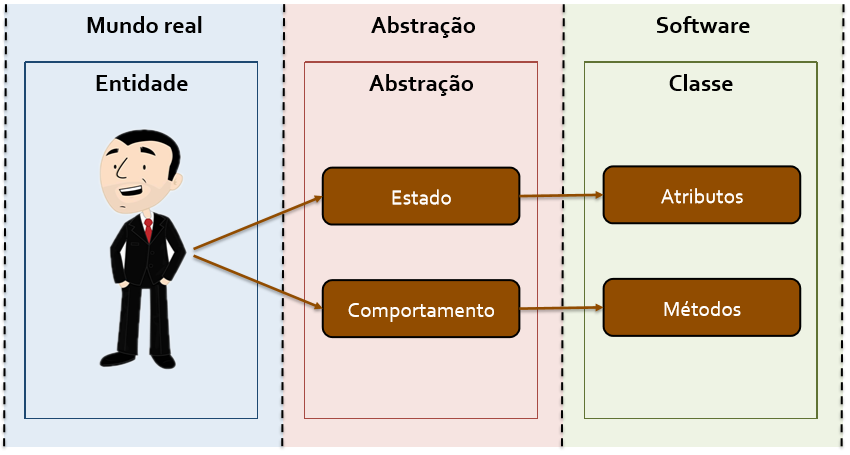
\includegraphics[width=0.6\textheight]{img/processo-abstracao.png}
	\caption{Processo de abstração para construção de classes}
	\label{fig:processo-abstracao}
\end{figure}

A Figura~\ref{fig:classe} apresenta a representação de uma classe que modela uma pessoa. Esta representação segue o padrões definidos pela UML (Unified Modeling Language). Como pode ser observado, a classe divide-se em três partes. A primeira mostra o nome da classe (Pessoa). Por padrão, o nome deve iniciar com letra maiúscula e seguir o formato camelCase. A segunda parte mostra os atributos da classe (sua estrutura), apresentando o nome de cada atributo, seu tipo e sua visibilidade (também chamado de modificador). Pode-se ainda apresentar um valor inicial para o atributo, como é feito com o atributo \texttt{sexo}. Finalmente, a terceira parte apresenta o conjunto de métodos da classe (seu comportamento), contendo o identificador do método, sua visibilidade, conjunto de parâmetros e tipo de retorno.

\begin{figure}[h]
	\centering
	\begin{tikzpicture}
	\umlclass{Pessoa}{ 
		-- id: int \\
		-- nome: String \\
		-- sexo: char = 'M' \\
		-- idade: int
	}{ 
		+ fazerAniversario(): void
	}
	\end{tikzpicture}
	\caption{Representação de uma classe usando UML}
	\label{fig:classe}
\end{figure}

No exemplo apresentado pela Figura~\ref{fig:classe}, o processo de abstração da entidade \code{Pessoa} resultou no conjunto de atributos composto pelo \code{id}, \code{nome}, \code{sexo} e \code{idade}, assim como o método de \code{fazerAniversario()}.

\section{Atributos e Métodos} 
Um \textbf{atributo} consiste em uma propriedade nomeada de uma classe e descreve a faixa de valores (tipo de dado) que pode assumir. Conforme discutido na seção anterior, os atributos definem as características (estrutura) presentes nos objetos da classe e dependem do domínio em questão. Cada objeto pode armazenar valores nos seus atributos. O conjunto de valores armazenados em um determinado momento constituem o estado do objeto.

Os \textbf{métodos} determinam o comportamento do objeto, ou seja, como ele age e reage, suas modificações de estado e interações com outros objetos. Além disso, eles definem o conjunto de operações que o objeto pode realizar. Estas operações podem ser solicitadas por outros objetos, conforme seus modificadores de acesso.

\section{Objetos} 
Objetos são instâncias de classes. Enquanto uma classe é uma abstração, um objeto é a manifestação concreta dessa abstração. Ou seja, é uma instância da entidade que possui um estado (valores dos seus atributos), comportamento (implementação dos seus métodos) e identidade. A Figura~\ref{fig:classe-objeto} mostra a classe \code{Pessoa} e um objeto desta classe (\code{maria}). Observe que o objeto pertence a uma classe (possui a estrutura e o comportamento definidos por ela) e apresenta valores nos seus atributos (estado).

\begin{figure}[h]
	\centering
	\begin{tikzpicture}
	\umlclass{Pessoa}{ 
		-- id: int \\
		-- nome: String \\
		-- sexo: char = 'M' \\
		-- idade: int
	}{ 
		+ fazerAniversario(): void
	}
	
	\umlclass[x=7]{maria:Pessoa}{ 
		id = 12 \\
		nome = "Maria Pereira" \\
		sexo = 'F' \\
		idade = 40
	}{}
	\end{tikzpicture}
	\caption{Representação de uma classe e o respectivo objeto}
	\label{fig:classe-objeto}
\end{figure}


\section{Implementação de classes}
Considerando o contexto de uma concessionária (sistema para gestão dos veículos), a classe \code{Veiculo} deve possuir: modelo, marca, ano, cor, potência e ar condicionado. Além disso, ela deve implementar um método para cálculo do imposto em função do ano do veículo. A Figura~\ref{fig:classe-veiculo} apresenta a classe \code{Veiculo} com os atributos e método supracitados.

\begin{figure}[h]
	\centering
	\begin{tikzpicture}
	\umlclass{Veiculo}{ 
		-- modelo: String \\
		-- marca: String \\
		-- ano: int \\
		-- potencia: double \\
		-- arCondicionado: boolean
	}{ 
		+ calculaImposto(): double
	}
	\end{tikzpicture}
	\caption{Representação UML da classe ``Veiculo''}
	\label{fig:classe-veiculo}
\end{figure}

O trecho de código abaixo mostra a implementação da classe apresentada pela Figura~\ref{fig:classe-veiculo}. A definição é feita pelas instruções \code{public class <nome-da-classe>}. Os atributos estão definidos nas linhas 3 a 7. Para cada atributo é definida sua visibilidade, seu tipo e o identificador (ex: \code{private String modelo}). O método da classe é definido nas linhas 9 a 13.

\begin{minted}{java}
public class Veiculo { 
	
	private String modelo; 
	private String marca; 
	private int ano; 
	private double potencia; 
	private boolean arCondicionado; 
	
	public double calculaImposto() { 
		if(ano < 2010) 
			return 500d; 
		return 700d; 
	} 
}
\end{minted}


\section{Encapsulamento}
Encapsular significa agrupar e empacotar os detalhes internos da abstração, tornando-os inacessíveis para entidades externas. Cada classe define a sua interface, composta pelos atributos e métodos que podem ser acessados/chamados a partir de objetos externos à classe. Neste sentido, encapsular consiste em definir quais elementos devem estar disponíveis a entidades externas, empacotando os detalhes daquilo que não deve estar disponível. A Figura~\ref{fig:encapsulamento} apresenta uma representação gráfica do conceito de encapsulamento.

\begin{figure}[h]
	\centering
	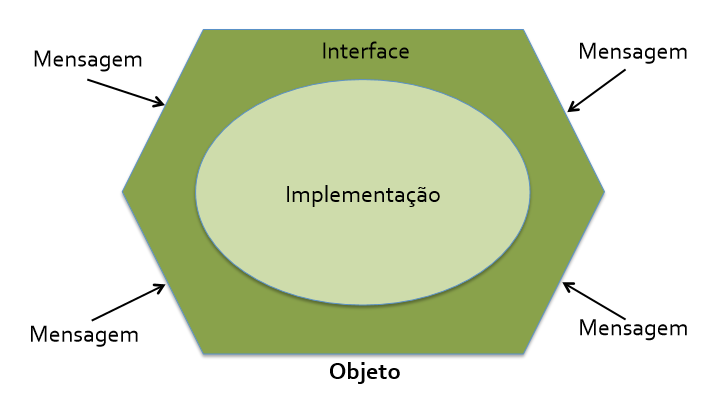
\includegraphics[width=0.6\textheight]{img/encapsulamento}
	\caption{Visão geral do conceito de encapsulamento}
	\label{fig:encapsulamento}
\end{figure}

Existem três principais modificadores de acesso:

\begin{itemize}
	\item \textbf{Privado (\texttt{-}):} O elemento é acessado apenas pela classe que o define.
	\item \textbf{Protegido (\texttt{\#}):} O elemento é acessado pela classe que o define e também por suas sub-classes.
	\item \textbf{Público (\texttt{+}):} Qualquer objeto pode acessar o elemento.
\end{itemize}

Os trechos de código abaixo exemplificam o uso do encapsulamento no atributo \code{saldo} da classe \code{ContaCorrente}. Na classe sem encapsulamento, o saldo pode ser acessado diretamente. Ou seja, o valor de saldo pode ser modificado por qualquer entidade externa (para a posterior realização de um saque, por exemplo). Este problema é corrigido na segunda classe, encapsulando o atributo \code{saldo}.

\begin{minted}{java}
//Classe sem encapsulamento
public class ContaBancaria {
	public double saldo;
	
	public boolean saque(double valor) {
		if(saldo >= valor) {
			saldo -= valor;
			return true;
		}
		return false;
	}	
}
\end{minted}

\begin{minted}{java}
//Classe com encapsulamento
public class ContaBancaria {
	private double saldo;

	public boolean saque(double valor) {
		if(saldo >= valor) {
			saldo -= valor;
			return true;
		}
		return false;
	}	
}
\end{minted}
 
 
\section{Métodos acessores}
Por conta do encapsulamento, os atributos das classes devem ser privados. Os métodos assessores (também conhecidos por métodos \code{get} e \code{set}) são responsáveis por devolver os valores dos atributos ou alterar seus valores, quando solicitado. 

Os métodos \code{get} (ex: \code{getNome()}) são responsáveis por devolver o valor de um atributo do objeto. Geralmente não possuem argumentos e possuem um tipo de retorno (o tipo do atributo). São públicos por padrão.

Os métodos \code{set} (ex: \code{setNome(String nome)}) são responsáveis por realizar a modificação dos valores dos atributos. Geralmente possuem como argumento o valor a ser atribuído e não possuem retorno. São públicos por padrão.

O trecho de código abaixo mostra o uso dos métodos acessores para acesso (recuperação e atribuição de valores) ao atributo \code{modelo} da classe \code{Veiculo}. Na linha 5, o argumento recebido pelo método \code{set} é armazenado no atributo \code{modelo}. Já na linha 9, o valor armazenado no atributo \code{modelo} é retornado pelo método \code{get}.

\begin{minted}{java}
public class Veiculo {
	private String modelo; 
	
	public void setModelo(String modelo) { 
		this.modelo = modelo; 
	} 
	
	public String getModelo() { 
		return this.modelo; 
	} 
}
\end{minted}


\section{Métodos construtores}

Quando um objeto é criado (ex: \code{pessoa = new Pessoa();}), um conjunto de passos é executado:

\begin{enumerate}
	\item Inicialização \texttt{default} dos campos (\texttt{null}, \texttt{false}, 0).
	\item Chamada recursiva aos construtores de cada superclasse (até \code{Object}).
	\begin{enumerate}
		\item Inicialização \texttt{default} dos campos das superclasses.
		\item Execução do conteúdo dos métodos construtores de cada superclasse (desde \code{Object}).
	\end{enumerate}
	\item \textbf{Execução do conteúdo do método construtor da classe.}
\end{enumerate}

Logo, o construtor é um método onde podemos definir o que será realizado quando um objeto da classe é criado. O método construtor não possui tipo de retorno e seu identificador é idêntico ao nome da classe. O trecho de código abaixo mostra a definição do método construtor da classe \code{Pessoa} (método \code{Pessoa()}). Com isso, cada objeto de \code{Pessoa} criado possui o valor \code{sem nome} no atributo \code{nome} e \code{1} no atributo \code{idade}.

\begin{minted}{java}
public class Pessoa { 
	
	private String nome; 
	private int idade; 
	
	public Pessoa() { 
		//Neste exemplo, são definidor valores 
		//iniciais para cada objeto criado 
		this.nome = "sem nome"; 
		this.idade = 1; 
	} 
}
\end{minted}

É possível (e comum) definir argumentos no método construtor, que são passados no momento em que o objeto é criado. Com isso, valores já podem ser armazenados nos atributos da instância. O trecho de código abaixo exemplifica a definição de um método construtor parametrizado para a classe \code{Pessoa}. Com isso, os valores recebidos como parâmetros são armazenados nos atributos da classe.

\begin{minted}{java}
public class Pessoa { 
	
	private String nome; 
	private int idade; 
	
	public Pessoa() { 
		this.nome = "Não especificado"; 
		this.idade = 1; 
	} 
	
	public Pessoa(String nome, int idade) { 
		this.nome = nome; 
		this.idade = idade; 
	} 
}
\end{minted}
 
Com isso, é possível definir dois ou mais métodos construtores, sem parâmetros ou com parâmetros. Esta técnica é chamada \textbf{sobrecarga de operações} e é discutida na Seção~\ref{sec:sobrecarga}. Quando não especificado um método construtor, o Java fornece um construtor padrão (sem argumentos e sem implementação). A partir do momento em que o programador define um método construtor, o construtor padrão deixa de existir.

\textbf{OBS:} o uso da instrução \code{this} serve para acessar a instância do objeto atual. É usado para diferenciar os atributos de variáveis locais.
 
 
\section{Métodos destrutores}
No Java, os objetos são destruídos (eliminados da memória) automaticamente, quando não existe mais nenhum ponteiro para ele. É possível definir um método a ser executado na destruição do objeto. Este método é o \code{finalize()} e suas instruções são executadas imediatamente antes da destruição do objeto. O trecho de código abaixo exemplifica seu uso.

\begin{minted}{java}
public class Pessoa {	  	
	private String nome;	  	
	private int idade;  	
	
	public void finalize(){	  	
		System.out.println("Objeto destruído: " + this.getNome());	
	}	
} 
\end{minted}

\section{Sobrecarga de operações}
\label{sec:sobrecarga}

Assim como os métodos construtores, métodos comuns também podem ser sobrecarregados. Ou seja, pode-se criar dois ou mais métodos com o mesmo identificador, desde que seus parâmetros sejam diferentes. Em outras palavras, a assinatura do método deve ser única. A assinatura é definida pelo identificador do método e os tipos dos seus parâmetros. O trecho de código a seguir mostra a sobrecarga do construtor da classe e também do método \code{soma}.
 
\begin{minted}{java}
public	class Acumulador{	
	private long somaInteiros;	
	
	public Acumulador() {		
		this.somaInteiros = 0;		
	}	
	
	public Acumulador(long valorInicial){		
		this.somaInteiros = valorInicial;	
	}	
	
	public void soma(int valor){	
		this.somaInteiros += valor;	
	}	
	
	public void soma(String valor) {		
		this.somaInteiros += Integer.parseInt(valor);	
	}	
} 
\end{minted}

No código anterior, os métodos \code{soma} possuem as assinaturas \code{void soma(int)} e \code{void soma(String)}, respectivamente. Dessa forma, o Java sabe qual dos dois métodos chamar, de acordo com o argumento passado a ele. Um terceiro método com um argumento do tipo \code{String} não seria permitido, pois sua assinatura seria idêntica a um dos métodos sobrecarregados. Ou seja, o Java não saberia qual dos dois chamar.

\section{Exemplo -- Compra}

Considere um sistema para gerenciar compras feitas pela Internet. O sistema deve armazenar os dados dos produtos comprados. A entidade envolvida neste sistema é apresentada pela Figura~\ref{fig:classe-compra}.

\begin{figure}[h]
	\centering
	\begin{tikzpicture}
	\umlclass{Compra}{ 
		-- produto: String \\
		-- precoUnitario: double \\
		-- quantidade: int \\
		-- enderecoEntrega: String \\
		-- status: String
	}{ 
		+ métodos construtores \\
		+ métodos set() e get() \\
		+ valorTotal(): double
	}
	\end{tikzpicture}
	\caption{Representação UML da classe ``Compra''}
	\label{fig:classe-compra}
\end{figure}

O trecho de código abaixo mostra a implementação da classe \code{Compra}. As linhas 3 a 7 implementam os atributos da classe, com modificador \code{private}. Ou seja, os atributos estão encapsulados e seu acesso é permitido através dos métodos acessores, também apresentados nos códigos abaixo. A classe ainda define dois métodos construtores: um vazio, e também sem implementação, e um parametrizado (linhas 9 a 18). Finalmente, a classe implementa um método \code{valorTotal}, que multiplica o preço unitário pela quantidade (linhas 20 a 22).

\begin{minted}{java}
public class Compra {

	private String produto;
	private double precoUnitario;
	private int quantidade;
	private String enderecoEntrega;
	private String status;
	
	public Compra() {}
	
	public Compra(String produto, double precoUnitario, int quantidade, String enderecoEntrega, String status) {
	
		this.produto = produto;
		this.precoUnitario = precoUnitario;
		this.quantidade = quantidade;
		this.enderecoEntrega = enderecoEntrega;
		this.status = status;
	}
	
	public double valorTotal() {
		return this.precoUnitario * this.quantidade;
	}
	
	public String getProduto() {
		return produto;
	}
	
	public void setProduto(String produto) {
		this.produto = produto;
	}
	
	public double getPrecoUnitario() {
		return precoUnitario;
	}
	
	public void setPrecoUnitario(double precoUnitario) {
		this.precoUnitario = precoUnitario;
	}
	
	public int getQuantidade() {
		return quantidade;
	}
	
	public void setQuantidade(int quantidade) {
		this.quantidade = quantidade;
	}
	
	public String getEnderecoEntrega() {
		return enderecoEntrega;
	}
	
	public void setEnderecoEntrega(String enderecoEntrega) {
		this.enderecoEntrega = enderecoEntrega;
	}
	
	public String getStatus() {
		return status;
	}
	
	public void setStatus(String status) {
		this.status = status;
	}
}
\end{minted}

O trecho de código abaixo mostra a implementação da classe \code{ExemploCompra}, que utiliza a classe \code{Compra} para suas operações. Nesta classe está a lista que armazena as compras efetuadas (\code{compras} -- linha 3). No método \code{main} são criados dois objetos da classe \code{Compra}. Na primeira vez, o objeto é instanciado e seus valores são atribuídos através dos métodos acessores (linhas 6 a 11). Na segunda vez, o objeto é criado e seus valores são passados no momento da criação, utilizando o construtor parametrizado (linha 15). Ambos os objetos, após criados, são inseridos na lista de compras (linhas 13 e 17). Finalmente, a lista é percorrida e os objetos são exibidos em tela (linhas 19 a 22).

\begin{minted}{java}
public class ExemploCompra {

	private static List<Compra> compras = new ArrayList<Compra>();
	
	public static void main(String[] args) {
		Compra compra = new Compra();
		compra.setProduto("Camiseta XPTO - TAM M");
		compra.setPrecoUnitario(140.0);
		compra.setQuantidade(2);
		compra.setEnderecoEntrega("Rua Getúlio Vargas, 200 - Ibirama, SC - 89140-000");
		compra.setStatus("Pedido realizado");
	
		compras.add(compra);
		
		Compra compra2 = new Compra("Tênis ABC 42", 300.0, 1, "Caixa Postal 27 - 89140-970", "Pagamento confirmado");
	
		compras.add(compra2);
	
		for(int i = 0; i < compras.size(); i++) {
			Compra c = compras.get(i);
			System.out.println("Compra: " + c.getProduto() + " a " + c.getPrecoUnitario() + "/unidade, totalizando " + c.valorTotal() + ".");
		}
	} 
}
\end{minted}

\begin{minipage}{\textwidth}
	\textbf{\texttt{SAÍDA:}}\\
	\texttt{Compra: Camiseta XPTO - TAM M a 140.0/unidade, totalizando 280.0.}\\
	\texttt{Compra: Tênis ABC 42 a 300.0/unidade, totalizando 300.0.}
\end{minipage}

\part{Relacionamentos entre classes}
\chapter{Visão geral}

\section{Tipos de relacionamentos}

As classes podem se conter relacionamentos entre si, definindo um vínculo entre seus objetos. Considerando as entidades em negrito, alguns exemplos de relacionamentos entre classes incluem:

\begin{itemize}
	\item Um \textbf{cliente} possui um \textbf{endereço}.
	\item Uma \textbf{empresa} é composta por \textbf{funcionários}.
	\item Uma \textbf{moto} é um tipo de \textbf{veículo}.
	\item Um \textbf{restaurante} possui \textbf{pratos}.
	\item Uma \textbf{correspondência} possui um \textbf{remetente} e um \textbf{destinatário}.
\end{itemize}

Existem diferentes tipos de relacionamentos. A lista abaixo resume os principais tipos de relacionamentos, os quais serão detalhados neste capítulo.

\begin{itemize}
	\item \textbf{Associação:} conexão entre classes.
	\item \textbf{Agregação e composição:} especialização de uma associação onde um todo é relacionado com suas partes (relacionamento ``todo-parte'').
	\item \textbf{Dependência:} um objeto depende de alguma forma de outro (relacionamento de utilização).
	\item \textbf{Herança (generalização):} um dos princípios da orientação a objetos, onde uma nova classe pode ser definida a partir de outra já existente (reutilização).
	\item \textbf{Realização:} um contrato que classe segue (obrigação).
\end{itemize}

\section{Representação UML}

A Figura~\ref{fig:relacionamentos-uml} mostra a representação UML dos relacionamentos supracitados. Uma associação é representada por um segmento de reta que une as duas classes. Os relacionamentos de agregação e composição são representados por uma reta com um losango no lado da entidade que representa o todo. A composição se difere da primeira por apresentar o losango preenchido. A dependência é representada por uma linha tracejada com uma ponta de seta aberta no lado da classe independente. A herança é representada por uma linha com uma ponta de seta fechada no lado da superclasse. Finalmente, a realização é representada da mesma forma que uma herança, com a diferença da reta ser tracejada. O restante deste capítulo discute cada relacionamento entre classes e apresenta sua implementação utilizando a linguagem Java.

\begin{figure}[h]
	\centering
	\begin{tikzpicture}
	\umlemptyclass{A}
	\umlemptyclass[x=6]{B}
	\umlassoc[name=associacao] {A}{B}
	
	\umlemptyclass[y=-2]{A}
	\umlemptyclass[x=6,y=-2]{B}
	\umlaggreg[name=agregacao] {A}{B}
	
	\umlemptyclass[y=-4]{A}
	\umlemptyclass[x=6,y=-4]{B}
	\umlcompo[name=composicao] {A}{B}
	
	\umlemptyclass[y=-6]{A}
	\umlemptyclass[x=6,y=-6]{B}
	\umlimport[name=dependencia] {A}{B}
	
	\umlemptyclass[y=-8]{A}
	\umlemptyclass[x=6,y=-8]{B}
	\umlinherit[name=heranca] {B}{A}
	
	\umlemptyclass[y=-10]{A}
	\umlemptyclass[x=6,y=-10]{B}
	\umlreal[name=realizacao] {A}{B}
	
	\node[above] at (associacao-1) {associação};
	\node[above] at (agregacao-1) {agregação};
	\node[above] at (composicao-1) {composição};
	\node[above] at (dependencia-1) {dependência};
	\node[above] at (heranca-1) {herança};
	\node[above] at (realizacao-1) {realização};
	
	\end{tikzpicture}
	\caption{Representação UML dos relacionamentos entre classes}
	\label{fig:relacionamentos-uml}
\end{figure}
\chapter{Associações simples}

Uma associação é uma conexão entre classes e representa uma relação entre os objetos envolvidos. Elas são representadas em um diagrama de classes através de uma linha, que conecta as classes associadas. Os dados podem fluir em uma ou em ambas as direções através do link. Existe dois duas formas principais de associação: com multiplicidade um (1) e com multiplicidade muitos (*). Cada uma das formas de associação pode ser implementada de forma unidirecional ou bidirecional.


\section{Associação com multiplicidade um (1)}

Uma associação de multiplicidade 1 ocorre quanto um objeto está vinculado a apenas um objeto da outra classe. Um exemplo deste tipo de associação é o vínculo existente entre um veículo (primeira entidade -- classe) e sua documentação (segunda entidade -- classe). Um veículo possui exatamente uma documentação, enquanto uma documentação pertence a exatamente um veículo. Logo, dizemos que este relacionamento é uma \textbf{associação de um para um}.

Na associação com multiplicidade 1, ao menos um dos atributos de uma das classes é do tipo da outra classe. Consideremos um exemplo envolvendo as classes \code{Veiculo} e \code{Documentacao}. Neste caso, o \code{Veiculo} possui um atributo do tipo \code{Documentacao} (\textbf{associação unidirecional de Veiculo para Documentacao}), ou a \code{Documentacao} possui um atributo do tipo \code{Veiculo} (\textbf{associação unidirecional de Documentacao para Veiculo}), ou ambos os casos (\textbf{associação bidirecional}).

\subsection{Caso unidirecional}

Consideremos o caso unidirecional. Se queremos que o atributo que implementa a associação fique na classe \code{Veiculo}, então temos uma associação unidirecional de \code{Veiculo} para \code{Documentacao}. Sua representação UML é apresentada na Figura~\ref{fig:associacao-uni-veiculo}. A direção da associação (chamada de navegabilidade) é informada através de uma ponta de seta. A navegabilidade representada na Figura~\ref{fig:associacao-uni-veiculo} mostra que a partir da classe \code{Veiculo} podemos chegar na classe \code{Documentacao}, pois existe um atributo na classe \code{Veiculo} do tipo \code{Documentacao}. Percebam que o atributo que implementa a associação não é representado no diagrama de classes, pois é implícito na representação da associação.

\begin{figure}[h]
	\centering
	
	\begin{tikzpicture}
	\umlclass{Veiculo}{
		-- modelo: String \\
		-- marca: String \\
		-- ano: int
		}{
		+ métodos set() e get()
		}
		
	\umlclass[x=8]{Documentacao}{
		-- renavam: int \\
		-- validade: int \\
		-- placa: String
		}{
		+ métodos set() e get()
		}
	
	\umluniassoc[geometry=-|-, mult1=1, mult2=1, pos2=2.8, align2=top]{Veiculo}{Documentacao}	
	\end{tikzpicture}
	
	\caption{Associação unidirecional de \texttt{Veiculo} para \texttt{Documentacao}}
	\label{fig:associacao-uni-veiculo}
\end{figure}

\textbf{OBS:} ao dizer que o veículo possui exatamente uma documentação, o vínculo é obrigatório. Ou seja, o atributo \code{documentacao} da classe \code{Veiculo} deve, obrigatoriamente, receber uma referência a um objeto da classe \code{Documentacao}. Caso quiséssemos modelar o relacionamento de tal forma que o veículo pudesse existir mesmo sem o vínculo com a documentação, então a multiplicidade do lado \code{Documentacao} deveria ser \code{0..1}.

Os trechos de código abaixo mostram a implementação das classes apresentadas no diagrama da Figura~\ref{fig:associacao-uni-veiculo} (os métodos construtores e demais métodos acessores foram omitidos). Reparem o atributo \code{doc} na classe \code{Veiculo}. Assim como os demais atributos, métodos acessores são definidos para acesso à documentação do veículo (ao atributo \code{doc}).
 
\begin{minted}{java}
public class Veiculo { 
	private String modelo; 
	private String marca; 
	private int ano; 
	private Documentacao doc; 

	public Documentacao getDoc() {
		return doc;
	}
	 
	public void setDoc(Documentacao doc) {
		this.doc = doc;
	}
	
	//demais métodos
}
\end{minted}

\begin{minted}{java}
public class Documentacao { 
	private int renavam; 
	private int validade;
	private String placa; 
	
	public int getRenavam() {
		return renavam;
	}
	 
	public void setRenavam(int renavam) {
		this.renavam = renavam;
	}
	
	//demais métodos
}
\end{minted}

O trecho de código a seguir mostra o uso da associação. Uma vez que as classes estejam associadas, devemos vincular os objetos no momento da sua criação (linha 4). Além disso, podemos acessar o vínculo para recuperar valores da documentação, a partir de um objeto da classe \code{Veiculo} (linha 5). Repare que não é possível acessar os dados do veículo a partir de um objeto da classe \code{Documentacao}, uma vez que o atributo que realiza a associação encontra-se na classe \code{Veiculo}.

\begin{minted}{java}
public static void main(String[] args) { 
	Veiculo carro = new Veiculo("Focus", "Ford", 2017); 
	Documentacao doc = new Documentacao(512647522, 2018, "QWD-2573"); 
	carro.setDoc(doc);
	System.out.println("O veículo " + carro.getModelo() + " possui placa " + carro.getDoc().getPlaca()); 
}
\end{minted}

Ainda no caso unidirecional, se quisermos que o atributo que implementa a associação fique na classe \code{Documentacao}, então temos uma associação unidirecional de \code{Documentacao} para \code{Veiculo}. Sua representação UML é apresentada na Figura~\ref{fig:associacao-uni-documentacao}. A direção da associação (navegabilidade) é apresentada pela ponta de seta, que aponta para a classe \code{Veiculo}. Neste caso, a partir da classe \code{Documentacao} podemos chegar na classe \code{Veiculo}, pois existe um atributo na classe \code{Documentacao} do tipo \code{Veiculo}.

\begin{figure}[h]
	\centering
	
	\begin{tikzpicture}
	\umlclass{Veiculo}{
		-- modelo: String \\
		-- marca: String \\
		-- ano: int
	}{
		+ métodos set() e get()
	}
	
	\umlclass[x=8]{Documentacao}{
		-- renavam: int \\
		-- validade: int \\
		-- placa: String
	}{
		+ métodos set() e get()
	}
	
	\umluniassoc[geometry=-|-, mult1=1, mult2=1, pos2=2.8, align2=top]{Documentacao}{Veiculo}	
	\end{tikzpicture}
	
	\caption{Associação unidirecional de \texttt{Documentacao} para \texttt{Veiculo}}
	\label{fig:associacao-uni-documentacao}
\end{figure}

\textbf{OBS:} novamente, ao dizer que a documentação é de exatamente um veículo, o vínculo é obrigatório. Ou seja, o atributo \code{veiculo} da classe \code{Documentacao} deve, obrigatoriamente, receber uma referência a um objeto da classe \code{Veiculo}. Caso quiséssemos modelar o relacionamento de tal forma que a documentação pudesse existir mesmo sem o vínculo com o veículo, então a multiplicidade do lado \code{Veiculo} deveria ser \code{0..1}.

Os trechos de código abaixo mostram a implementação das classes apresentadas no diagrama da Figura~\ref{fig:associacao-uni-documentacao} (os métodos construtores e demais métodos acessores foram omitidos). Reparem o atributo \code{veiculo} na classe \code{Documentacao}. Assim como os demais atributos, métodos acessores são definidos para acesso ao veículo da documentação (ao atributo \code{veiculo}).

\begin{minted}{java}
public class Veiculo {
	private String modelo;
	private String marca;
	private int ano;
	
	public String getModelo() {
		return modelo;
	}
	
	public void setModelo(String modelo) {
		this.modelo = modelo;
	}
	
	//demais métodos
}
\end{minted}

\begin{minted}{java}
public class Documentacao {
	private int renavam;
	private int validade;
	private String placa;
	private Veiculo veiculo;
	
	public Veiculo getVeiculo() {
		return veiculo;
	}
	
	public void setVeiculo(Veiculo veiculo){
		this.veiculo = veiculo;
	}
	
	//demais métodos
}
\end{minted}

O trecho de código a seguir mostra o uso da associação. Analogamente ao exemplo anterior, podemos acessar o vínculo para recuperar valores do veículo a partir de um objeto da classe \code{Documentacao} (linha 5). Repare que não é possível acessar os dados da documentação a partir de um objeto da classe \code{Veiculo}, uma vez que o atributo que realiza a associação encontra-se na classe \code{Documentacao}.

\begin{minted}{java}
public static void main(String[] args) {
	Veiculo carro = new Veiculo("Focus", "Ford", 2017);
	Documentacao doc = new Documentacao(512647522, 2018, "QWD-2573");
	doc.setVeiculo(carro);
	System.out.println("O documento " + doc.getRenavam() + " pertence ao veículo " + doc.getVeiculo().getModelo());
}
\end{minted}

\subsection{Caso bidirecional}

Se quisermos que ambas as classes possuam atributos que implementem o vínculo, podemos adotar uma associação bidirecional. Neste caso, existe um atributo da classe \code{Veiculo} na classe \code{Documentacao}, bem como um atributo da classe \code{Documentacao} na classe \code{Veiculo}. Com isso, é possível acessar a documentação a partir da classe \code{Veiculo}, bem como acessar o veículo a partir da classe \code{Documentacao}. Na UML, representamos uma associação bidirecional aplicando a ponta de seta nos dois lados da linha, ou omitindo a ponta de seta e mantendo uma linha simples (neste caso, entende-se que a associação é bidirecional). A Figura~\ref{fig:associacao-bidirecional} mostra as duas opções de representação UML de um relacionamento de associação bidirecional.

\begin{figure}[h]
	\centering
	
	\begin{tikzpicture}
	\umlclass{Veiculo}{
		-- modelo: String \\
		-- marca: String \\
		-- ano: int
	}{
		+ métodos set() e get()
	}
	
	\umlclass[x=8]{Documentacao}{
		-- renavam: int \\
		-- validade: int \\
		-- placa: String
	}{
		+ métodos set() e get()
	}
	
	\umlassoc[geometry=-|-, mult1=1, mult2=1, pos2=2.8, align2=top]{Documentacao}{Veiculo}	
	
	\umlclass[y=-4]{Veiculo}{
		-- modelo: String \\
		-- marca: String \\
		-- ano: int
	}{
		+ métodos set() e get()
	}
	
	\umlclass[x=8,y=-4]{Documentacao}{
		-- renavam: int \\
		-- validade: int \\
		-- placa: String
	}{
		+ métodos set() e get()
	}
	
	\umluniassoc[geometry=-|-, mult1=1, mult2=1, pos2=2.8, align2=top]{Documentacao}{Veiculo}	
	\umluniassoc[geometry=-|-]{Veiculo}{Documentacao}	
	\end{tikzpicture}
	
	\caption{Associação unidirecional de \texttt{Documentacao} para \texttt{Veiculo}}
	\label{fig:associacao-bidirecional}
\end{figure}

Os trechos de código abaixo mostram a implementação da associação bidirecional entre \code{Veiculo} e \code{Documentacao}. Repare nos atributos \code{doc} (classe \code{Veiculo}) e \code{veiculo} (classe \code{Documentacao}), os quais implementam o vínculo bidirecional e permite a navegação em ambos os sentidos.

 \begin{minted}{java}
public class Veiculo {
	private String modelo;
	private String marca;
	private int ano;
	private Documentacao doc;
	
	public Documentacao getDoc() {
		return doc;
	}
	
	public void setDoc(Documentacao doc) {
		this.doc = doc;
	}
	
	//demais métodos
}
\end{minted}

\begin{minted}{java}
public class Documentacao {
	private int renavam;
	private int validade;
	private String placa;
	private Veiculo veiculo;
	
	public Veiculo getVeiculo() {
		return veiculo;
	}
	
	public void setVeiculo(Veiculo veiculo){
		this.veiculo = veiculo;
	}
	
	//demais métodos
}
\end{minted}

O código a seguir mostra o uso das entidades com a associação bidirecional. Após a criação dos objetos, eles são vinculados nas linhas 4 e 5. Perceba que é preciso atribuir o veículo à sua documentação, e também a documentação ao seu veículo, uma vez que a associação é bidirecional. Após isso, é possível acessar os dados do veículo a partir da documentação (linha 6), bem como acessar os dados da documentação a partir do veículo (linha 7).

\begin{minted}{java}
public static void main(String[] args) {
	Veiculo carro = new Veiculo("Focus", "Ford", 2017);
	Documentacao doc = new Documentacao(512647522, 2018, "QWD-2573");
	doc.setVeiculo(carro);
	carro.setDoc(doc);
	System.out.println(doc.getRenavam() + " pertence ao " + doc.getVeiculo().getModelo());
	System.out.println(carro.getModelo() + " possui placa " + carro.getDoc().getPlaca());
}
\end{minted}

 
\section{Exemplo -- Gerente e Sala}
 
Consideremos as entidades \code{Gerente} e \code{Sala}. Cada gerente possui uma sala de trabalho. Cada sala é ocupada por, no máximo, um gerente. Logo, as entidades possuem uma associação, cuja multiplicidade máxima é 1. No entanto, neste caso um gerente pode não trabalhar em uma sala (caso seja um gerente externo, por exemplo). Além disso, uma sala pode não possuir nenhum gerente que trabalhe nela (uma sala vazia, por exemplo). Podemos informar a possibilidade de haver estes casos no próprio diagrama de classes, atribuindo multiplicidade \code{0..1}, ou seja, um gerente possui zero ou uma sala. Com isso, a chamada para vínculo dos objetos não é obrigatória e o atributo que implementa a associação pode não receber um vínculo (armazenar valor \code{null}).

Se desejarmos que a entidade \code{Gerente} tenha acesso aos dados da sua sala e, ao mesmo tempo, a entidade \code{Sala} tenha acesso aos dados do gerente que trabalha nela, podemos optar por uma associação bidirecional. O diagrama apresentado pela Figura~\ref{fig:gerente-sala} modela esta situação. As classes possuem uma associação bidirecional com multiplicidade \code{0..1} nos dois lados. Com isso, um gerente trabalha em uma sala ou em nenhuma sala, enquanto uma sala é habitada por um gerente, ou por nenhum gerente.

\begin{figure}[h]
	\centering
	
	\begin{tikzpicture}
	\umlclass{Gerente}{
		-- matricula: int \\
		-- nome: String \\
		-- funcao: String
	}{
		+ métodos set() e get()
	}
	
	\umlclass[x=8]{Sala}{
		-- numero: int \\
		-- predio: int \\
		-- andar: int
	}{
		+ métodos set() e get()
	}
	
	\umlassoc[geometry=-|-, mult1=0..1, mult2=0..1, pos1=0.25, pos2=2.75, align2=top]{Gerente}{Sala}
	\end{tikzpicture}
	
	\caption{Diagrama de classes para o exemplo \texttt{Sala} e \texttt{Gerente}}
	\label{fig:gerente-sala}
\end{figure}

Os techos de código abaixo mostram a implementação das classes \code{Gerente} e \code{Sala}. Os métodos \code{setSala} e \code{setGerente} foram implementados de tal forma que permita a chamada de uma única instrução, sem exigir que o programador faça o vínculo dos dois lados. Com isso, o programador se preocupa apenas em chamar o método \code{setSala} (da classe \code{Gerente}), que armazena o objeto recebido como parâmetro no atributo \code{sala} (linha 27) e, caso o parâmetro não seja \code{null}, atribui a si mesmo como gerente da sala (linhas 28 a 30), fazendo o vínculo nos dois lados. Já o método \code{setGerente} verifica se o parâmetro recebido não é \code{null}, neste caso o gerente antes vinculado a esta sala recebe \code{null} como sala, pois um novo gerente trabalhará nesta sala (linha 21). Finalmente, o novo gerente é atribuído (linha 22).
 
\begin{minted}{java}
public class Gerente {
	private int matricula;
	private String nome;
	private String funcao;
	private Sala sala;
	
	public Gerente() {}
	
	public Gerente(int matricula, String nome, String funcao) {
		this.matricula = matricula;
		this.nome = nome;
		this.funcao = funcao;
	}
	
	public Gerente(int matricula, String nome, String funcao, Sala sala) {
		this.matricula = matricula;
		this.nome = nome;
		this.funcao = funcao;
		setSala(sala);
	}
	
	public Sala getSala() {
		return sala;
	}
	
	public void setSala(Sala sala) {
		this.sala = sala;
		if(sala != null)
			sala.setGerente(this);
		}
	}
	
	//demais métodos acessores
}
\end{minted}
 
\begin{minted}{java}
public class Sala {
	private int numero;
	private String predio;
	private int andar;
	private Gerente gerente;
	
	public Sala() {}
	
	public Sala(int numero, String predio, int andar) {
		this.numero = numero;
		this.predio = predio;
		this.andar = andar;
	}
	
	public Gerente getGerente() {
		return gerente;
	}
	
	public void setGerente(Gerente gerente) {
		if(this.gerente != null)
			this.gerente.setSala(null);
			this.gerente = gerente;
		}
	}
	
	//demais métodos acessores
}
\end{minted}
 
Uma boa prática consiste em separar as funcionalidades do programa da classe que implementa o método \code{main}. Nos exemplos abaixo, o método \code{main} é implementado pela classe \code{Principal}, enquanto as funcionalidades do sistema são implementadas pela classe \code{Exemplo}. Esta classe ainda implementa um método \code{run}, que chama os métodos e as instruções desejadas (poderia apresentar um menu ao usuário, por exemplo). O método \code{main} apenas cria um objeto da classe \code{Exemplo} e chama o seu método \code{run}. Ou seja, a função do método \code{main} se limira a iniciar a aplicação.
 
\begin{minted}{java}
public class Principal {
	public static void main(String[] args) {
		Exemplo exemplo = new Exemplo();
		exemplo.run();
	}
}
\end{minted}
 
\begin{minted}{java}
public class Exemplo {
	private List<Sala> salas = new ArrayList<Sala>();
	private List<Gerente> gerentes = new ArrayList<Gerente>();

	public void run() {
		insereSalas();
		insereGerentes();
		mostraRegistros();
	}

	public void insereSalas() {
		Sala sala1 = new Sala(101, "Alpha", 1);
		Sala sala2 = new Sala(102, "Alpha", 1);
		Sala sala3 = new Sala(205, "Alpha", 2);
		Sala sala4 = new Sala(346, "Beta", 5);
		Sala sala5 = new Sala(12, "Gamma", 3);

		salas.add(sala1);
		salas.add(sala2);
		salas.add(sala3);
		salas.add(sala4);
		salas.add(sala5);
	}

	public void insereGerentes() {
		Gerente gerente1 = new Gerente(123456, "José da Silva", "Compras");
		Gerente gerente2 = new Gerente(654321, "Maria Pereira", "Vendas");
		Gerente gerente3 = new Gerente(123789, "João Assunção", "Marketing");
		Gerente gerente4 = new Gerente(987321, "Ana Maria Rodrigues", "Produção");

		gerente1.setSala(salas.get(0));
		gerente2.setSala(salas.get(1));
		gerente3.setSala(salas.get(2));
		gerente4.setSala(salas.get(0));

		gerentes.add(gerente1);
		gerentes.add(gerente2);
		gerentes.add(gerente3);
		gerentes.add(gerente4);
	}

	public void mostraRegistros() {
		for(Gerente g : gerentes) {
			if(g.getSala() != null)
				System.out.println(g.getNome() + " trabalha na sala " + g.getSala().getNumero() + " do prédio " + g.getSala().getPredio() + ".");
			else
				System.out.println(g.getNome() + " não possui uma sala de trabalho.");
		}

		System.out.println("");

		for(Sala s : salas) {
			if(s.getGerente() != null)
				System.out.println("Na sala " + s.getNumero() + " do prédio " + s.getPredio() + " trabalha " + s.getGerente().getNome() + ".");
			else
				System.out.println("Na sala " + s.getNumero() + " do prédio " + s.getPredio() + " não trabalha nenhum gerente.");
		}
	}
}
\end{minted}

O método \code{insereSalas} cria um conjunto de salas e insere na lista de salas. O método \code{insereGerentes} cria um conjunto de gerentes, vincula a algumas das salas criadas pelo método anterior e os insere na lista de gerentes. Repare que o vínculo é feito apenas pelo método \code{setSala}, dada a implementação apresentada anteriormente. O método \code{mostraRegistros} percorre a lista de gerentes e apresenta seu nome, a sala e o prédio onde trabalha. Caso ele não esteja vinculado a nenhuma sala (quando o atributo \code{sala} é \code{null}), é apresentada a mensagem de que o mesmo não possui sala de trabalho. Depois disso, a lista de salas é percorrida, apresentando o número da sala e seu prédio, juntamente com o nome do gerente que ocupa esta sala. Caso a sala esteja vazia (o atributo \code{gerente} é \code{null}), é apresentada a mensagem de que na referida sala não trabalha nenhum gerente.

\begin{minipage}{\textwidth}
	\textbf{\texttt{SAÍDA:}}\\
	\texttt{José da Silva não possui uma sala de trabalho.}\\
	\texttt{Maria Pereira trabalha na sala 102 do prédio Alpha.}\\
	\texttt{João Assunção trabalha na sala 205 do prédio Alpha.}\\
	\texttt{Ana Maria Rodrigues trabalha na sala 101 do prédio Alpha.}\\
	\\
	\texttt{Na sala 101 do prédio Alpha trabalha Ana Maria Rodrigues.}\\
	\texttt{Na sala 102 do prédio Alpha trabalha Maria Pereira.}\\
	\texttt{Na sala 205 do prédio Alpha trabalha João Assunção.}\\
	\texttt{Na sala 346 do prédio Beta não trabalha nenhum gerente.}\\
	\texttt{Na sala 12 do prédio Gamma não trabalha nenhum gerente.}
\end{minipage}

\section{Associação com multiplicidade muitos (*)}
 
A associação com multiplicidade muitos (*) ocorre quanto um objeto está vinculado a vários objetos da outra classe. Um exemplo deste tipo de associação é o vínculo existente entre uma empresa (primeira entidade -- classe) e seus funcionários (segunda entidade -- classe). Um funcionário trabalha em uma empresa, e uma empresa possui vários (ou muitos) funcionários. Perceba que, agora, um objeto da classe \code{Empresa} está associado a vários objetos da classe \code{Funcionario}. Logo, dizemos que este relacionamento é uma \textbf{associação de um para muitos}.

Como em qualquer associação, os dados podem fluir em uma ou em ambas as direções através do link. Isto é, podemos implementar uma associação com multiplicidade muitos tanto na forma unidirecional, quanto bidirecional. Podemos utilizar um atributo da classe \code{Empresa} na classe \code{Funcionario} (\textbf{associação unidirecional de Funcionario para Empresa}), ou uma lista de objetos da classe \code{Funcionario} na classe \code{Empresa} (\textbf{associação unidirecional de Empresa para Funcionario}), ou ambos os casos (\textbf{associação bidirecional}). 

Repare que no caso de multiplicidade muitos, existem casos em que se faz necessário implementar a associação utilizando uma lista de objetos da outra classe. Este é o caso onde, a partir de uma empresa, desejamos obter os dados dos seus funcionários. Como a empresa não possui apenas um funcionário, não é possível implementar a associação com um objeto simples. Logo, uma lista de funcionários permite o armazenamento dos diversos funcionários da empresa.

\subsection{Caso unidirecional}

Consideremos o caso unidirecional. Se quisermos que o vínculo seja implementado pela classe \code{Empresa}, então temos uma associação unidirecional de \code{Empresa} para \code{Funcionario}. Sua representação UML é apresentada na Figura~\ref{fig:associacao-muitos-uni-empresa}.

\begin{figure}[h]
	\centering
	
	\begin{tikzpicture}
	\umlclass{Empresa}{
		-- razaoSocial: String \\
		-- nomeFantasia: String \\
		-- cnpj: String
	}{
		+ métodos set() e get()
	}
	
	\umlclass[x=8]{Funcionario}{
		-- nome: String \\
		-- cpf: String
	}{
		+ métodos set() e get()
	}
	
	\umluniassoc[geometry=-|-, mult1=1, mult2=*, pos1=0.2, pos2=2.75, align2=top]{Empresa}{Funcionario}
	\end{tikzpicture}
	
	\caption{Associação unidirecional de \texttt{Empresa} para \texttt{Funcionario}}
	\label{fig:associacao-muitos-uni-empresa}
\end{figure}

Neste caso, precisamos implementar uma lista de objetos de \code{Funcionario} na classe \code{Empresa}. Os trechos de código abaixo mostram a implementação de ambas as classes para este caso. Uma boa prática consiste em definir um método específico para adicionar um objeto na lista. Este método é apresentado nas linhas 7 a 9 da classe \code{Empresa}. Sempre que for necessário vincular um funcionário à empresa, este método pode (ou deve) ser utilizado.

\textbf{OBS:} podemos substituir a multiplicidade muitos por \code{0..*} ou \code{1..*}, definindo o mínimo de objetos que a lista deve conter. No caso da multiplicidade \code{0..*} a lista pode conter nenhum, um ou muitos objetos vinculados. No caso da multiplicidade \code{1..*}, a lista deve conter ao menos um objeto vinculado.

\begin{minted}{java}
public class Empresa {
	private String razaoSocial;
	private String nomeFantasia;
	private String cnpj;
	private List<Funcionario> funcionarios;

	public Empresa() {
		funcionarios = new ArrayList<Funcionario>();
	}

	public void addFuncionario(Funcionario f) {
		this.funcionarios.add(f);
	}
	
	//demais métodos
}
\end{minted}

\begin{minted}{java}
public class Funcionario {
	private String nome;
	private String cpf;

	public String getNome() {
		return nome;
	}

	public void setNome(String nome) {
		this.nome = nome;
	}
	
	//demais métodos
}
\end{minted}

O trecho de código a seguir mostra o uso da associação implementada. São criados distintos objetos das classes \code{Funcionario} e \code{Empresa} (linhas 2 a 7). Após isso, os funcionários são atribuídos às respectivas empresas utilizando o método \code{addFuncionario} (linhas 9 a 11). Finalmente, todos os funcionários da empresa \code{e1} são apresentados (linhas 13 e 14). Perceba que a lista de funcionários da empresa \code{e1} é recuperada e, então, seus dados são apresentados em tela.

\begin{minted}{java}
public static void main(String[] args) {
	Funcionario f1 = new Funcionario("José da Silva", "012.541.379-33");
	Funcionario f2 = new Funcionario("Maria Pereira", "062.411.632-12");
	Funcionario f3 = new Funcionario("Pedro Ferreira", "178.219.475-25");
	
	Empresa e1 = new Empresa("Empresa 1 LTDA", "Empresa 1", "123.456.789/0001-01");
	Empresa e2 = new Empresa("Empresa 2 LTDA", "Empresa 2", "123.456.789/0001-02");
	
	e1.addFuncionario(f1);
	e1.addFuncionario(f2);
	e2.addFuncionario(f3);
	
	for(Funcionario f : e1.getFuncionarios())
		System.out.println(f.getNome() + " é funcionário na " + e1.getNomeFantasia());
}
\end{minted}

A mesma análise anterior pode ser feita na associação com multiplicidade muitos. Mantendo uma lista de funcionários para cada empresa, podemos acessar os dados dos funcionários a partir da classe \code{Empresa}. Porém, não é possível acessar os dados da empresa a partir da classe \code{Funcionario}. Para modificar isso, podemos inverter a navegabilidade da associação, de modo a manter o vínculo na classe \code{Funcionario}. Neste caso, o funcionário tem um atributo simples do tipo \code{Empresa}. Este caso está representado no diagrama da Figura~\ref{fig:associacao-muitos-uni-funcionario} e sua implementação segue os conceitos apresentados nas seções anteriores, podendo ser observada nos códigos abaixo.

\textbf{OBS:} como a multiplicidade indica que o funcionário pertence a exatamente uma empresa, o vínculo é obrigatório.

\begin{figure}[h]
	\centering
	
	\begin{tikzpicture}
	\umlclass{Empresa}{
		-- razaoSocial: String \\
		-- nomeFantasia: String \\
		-- cnpj: String
	}{
		+ métodos set() e get()
	}
	
	\umlclass[x=8]{Funcionario}{
		-- nome: String \\
		-- cpf: String
	}{
		+ métodos set() e get()
	}
	
	\umluniassoc[geometry=-|-, mult1=*, mult2=1, pos1=0.2, pos2=2.75, align2=top]{Funcionario}{Empresa}
	\end{tikzpicture}
	
	\caption{Associação unidirecional de \texttt{Funcionario} para \texttt{Empresa}}
	\label{fig:associacao-muitos-uni-funcionario}
\end{figure}

\begin{minted}{java}
public class Empresa {
	private String razaoSocial;
	private String nomeFantasia;
	private String cnpj;
	
	public String getRazaoSocial() {
		return razaoSocial; 
	}
	
	public void setRazaoSocial(String r) {
		this.razaoSocial = r; 
	}
}
\end{minted}

\begin{minted}{java}
public class Funcionario {
	private String nome;
	private String cpf;
	private Empresa empresa;
	
	public Empresa getEmpresa() {
		return empresa; 
	}
	
	public void setEmpresa(Empresa empresa) {
		this.empresa = empresa;
	}
}
\end{minted}

\begin{minted}{java}
public static void main(String[] args) {
	Funcionario f1 = new Funcionario("José da Silva", "012.541.379-33");
	Funcionario f2 = new Funcionario("Maria Pereira", "062.411.632-12");
	Funcionario f3 = new Funcionario("Pedro Ferreira", "178.219.475-25");
	
	Empresa e1 = new Empresa("Empresa 1 LTDA", "Empresa 1", "123.456.789/0001-01");
	Empresa e2 = new Empresa("Empresa 2 LTDA", "Empresa 2", "123.456.789/0001-02");
	
	f1.setEmpresa(e1);
	f2.setEmpresa(e1);
	f3.setEmpresa(e2);
	
	System.out.println(f1.getNome() + " é func. na " + f1.getEmpresa().getNomeFantasia());
	System.out.println(f2.getNome() + " é func. na " + f2.getEmpresa().getNomeFantasia());
	System.out.println(f3.getNome() + " é func. na " + f3.getEmpresa().getNomeFantasia());
}
\end{minted}
 
\subsection{Caso bidirecional}

Se quisermos que ambas as classes possuam atributos que implementem o vínculo, podemos adotar uma associação bidirecional. Neste caso, existe uma lista de objetos de \code{Funcionario} na classe \code{Empresa}, e um objeto da classe \code{Empresa} na classe \code{Funcionario}. Com isso, é possível acessar todos os funcionários de uma empresa, bem como a empresa em que um determinado funcionário trabalha. A Figura~\ref{fig:associacao-bidirecional-empresa} apresenta a representação UML com relacionamento bidirecional entre as classes.

\begin{figure}[h]
	\centering
	
	\begin{tikzpicture}
	\umlclass{Empresa}{
		-- razaoSocial: String \\
		-- nomeFantasia: String \\
		-- cnpj: String
	}{
		+ métodos set() e get()
	}
	
	\umlclass[x=8]{Funcionario}{
		-- nome: String \\
		-- cpf: String
	}{
	+ métodos set() e get()
	}
	
	\umlassoc[geometry=-|-, mult1=1, mult2=*, pos1=0.2, pos2=2.75, align2=top]{Funcionario}{Empresa}
	\end{tikzpicture}
	
	\caption{Associação bidirecional entre \texttt{Empresa} e \texttt{Funcionario}}
	\label{fig:associacao-bidirecional-empresa}
\end{figure}
 
Os trechos de código a seguir mostram a implementação da estrutura de classes apresentada na Figura~\ref{fig:associacao-bidirecional-empresa}. Repare nos atributos que implementam o vínculo bidimensional. Na classe \code{Empresa} temos a lista de funcionários (\code{funcionarios}), enquanto na classe \code{Funcionario} temos o vínculo com a empresa (\code{empresa}). Repare ainda que o método \code{setEmpresa} da classe \code{Funcionario} também realiza a operação de inclusão do funcionário na lista de funcionários da empresa.

\begin{minted}{java}
public class Empresa {
	private String razaoSocial;
	private String nomeFantasia;
	private String cnpj;
	private List<Funcionario> funcionarios;
	
	public void addFuncionario(Funcionario f){
		this.funcionarios.add(f);
	}
}
\end{minted}

\begin{minted}{java}
public class Funcionario {
	private String nome;
	private String cpf;
	private Empresa empresa;
	
	public void setEmpresa(Empresa empresa){
		this.empresa = empresa;
		empresa.addFuncionario(this);
	}
}
\end{minted} 

O código abaixo mostra o uso da estrutura proposta. A atribuição é feita pela chamada do método \code{setEmpresa} (linhas 9 a 11). As linhas 13 a 15 mostram que é possível acessar todos os funcionários da empresa (\code{e1.getFuncionarios()}), bem como acessar os dados da empresa em que um funcionário trabalha (\code{f.getEmpresa().getNomeFantasia()}).

\begin{minted}{java}
public static void main(String[] args) {
	Funcionario f1 = new Funcionario("José da Silva", "012.541.379-33");
	Funcionario f2 = new Funcionario("Maria Pereira", "062.411.632-12");
	Funcionario f3 = new Funcionario("Pedro Ferreira", "178.219.475-25");

	Empresa e1 = new Empresa("Empresa 1 LTDA", "Empresa 1", "123.456.789/0001-01");
	Empresa e2 = new Empresa("Empresa 2 LTDA", "Empresa 2", "123.456.789/0001-02");

	f1.setEmpresa(e1);
	f2.setEmpresa(e1);
	f3.setEmpresa(e2);

	for(Funcionario f : e1.getFuncionarios())
		 System.out.println(f.getNome() + " trabalha na " + f.getEmpresa().getNomeFantasia());
}
\end{minted}

\section{Exemplo -- Clube e Sócio}

Considere o contexto de um clube e seus sócios, onde um clube possui vários sócios. O diagrama de classes é apresentado pela Figura~\ref{fig:exemplo-clube-socio}. Pela navegabilidade proposta, a classe \code{Clube} possui uma lista de objetos da classe \code{Socio}, podendo essa lista ser vazia (multiplicidade \code{0..*}).

\begin{figure}[h]
	\centering
	
	\begin{tikzpicture}
	\umlclass{Clube}{
		-- nome: String \\
		-- cidade: String
	}{
		+ métodos set() e get()
	}
	
	\umlclass[x=8]{Socio}{
		-- matricula: int \\
		-- nome: String \\
		-- idade: int
	}{
		+ métodos set() e get()
	}
	
	\umluniassoc[geometry=-|-, mult1=1, mult2=0..*, pos1=0.1, pos2=2.75, align2=top]{Clube}{Socio}
	\end{tikzpicture}
	
	\caption{Diagrama de classes para \texttt{Clube} e \texttt{Socio}}
	\label{fig:exemplo-clube-socio}
\end{figure}

Os trechos de código abaixo mostram a implementação das classes \code{Clube} e \code{Socio}. Perceba que a lista que implementa a associação encontra-se na classe \code{Clube} (linha 4), conforme definido na navegabilidade. Esta classe ainda implementa o método \code{addSocio}, responsável por inserir o sócio recebido como argumento na lista. Além disso, a classe implementa o método \code{removeSocio}, que recebe a matrícula do sócio a ser removido, busca o objeto desejado na lista e o remove, caso encontrado. Este método devolve verdadeiro, em caso de sucesso, e falso, caso contrário.

\begin{minted}{java}
public class Clube {
	private String nome;
	private String cidade;
	private List<Socio> socios;

	public Clube() {
		socios = new ArrayList<Socio>();
	}

	public Clube(String nome, String cidade) {
		this.nome = nome;
		this.cidade = cidade;
		this.socios = new ArrayList<Socio>();
	}

	public void addSocio(Socio socio) {
		this.socios.add(socio);
	}

	public boolean removeSocio(int matricula) {
		for(Socio s : socios) {
			if(s.getMatricula() == matricula) {
				this.socios.remove(s);
				return true;
			}
		}
		return false;
	}

	public List<Socio> getSocios() {
		return socios;
	}

	public void setSocios(List<Socio> socios) {
		this.socios = socios;
	}

	public String getNome() {
		return nome;
	}

	public void setNome(String nome) {
		this.nome = nome;
	}

	public String getCidade() {
		return cidade;
	}

	public void setCidade(String cidade) {
		this.cidade = cidade;
	}
}
\end{minted}

\begin{minted}{java}
public class Socio {
	private int matricula;
	private String nome;
	private int idade;

	public Socio() {}

	public Socio(int matricula, String nome, int idade) {
		this.matricula = matricula;
		this.nome = nome;
		this.idade = idade;
	}

	public int getMatricula() {
		return matricula;
	}

	public void setMatricula(int matricula) {
		this.matricula = matricula;
	}

	public String getNome() {
		return nome;
	}

	public void setNome(String nome) {
		this.nome = nome;
	}

	public int getIdade() {
		return idade;
	}

	public void setIdade(int idade) {
		this.idade = idade;
	}
}
\end{minted}

Os trechos de código a seguir mostram o uso da estrutura de classes apresentada acima. O método \code{insereRegistros} é responsável por criar, vincular e armazenar os registros nas listas definidas na classe \code{Aplicacao}. O método \code{removeSocio} seleciona um clube e um sócio, e faz a remoção do sócio da lista de sócios do clube. Em caso de sucesso, o sócio é removido também da lista geral de sócios. O método \code{mostraRegistros} percorre a lista de clubes, acessando seus dados e sua lista de sócios, para apresentação em tela.

\begin{minted}{java}
public class Principal {
	public static void main(String[] args) {
		Exemplo exemplo = new Exemplo();
		exemplo.run();
	}
}	
\end{minted}

\begin{minted}{java}
public class Exemplo {
	private List<Socio> socios = new ArrayList<Socio>();
	private List<Clube> clubes = new ArrayList<Clube>();

	public void run() {
		insereRegistros();
		removeSocio();
		mostraRegistros();
	}

	private void insereRegistros() {
		Socio s1 = new Socio(123456, "Maria da Rosa", 45);
		Socio s2 = new Socio(654321, "José da Silva", 25);
		Socio s3 = new Socio(147852, "Ana Lúcia da Silva", 30);
		Socio s4 = new Socio(369852, "Pedro Ferreira", 28);
		socios.add(s1);
		socios.add(s2);
		socios.add(s3);
		socios.add(s4);

		Clube c1 = new Clube("Clube ABC", "Ibirama");
		Clube c2 = new Clube("Clube XYZ", "Blumenau");
		clubes.add(c1);
		clubes.add(c2);

		c1.addSocio(s1);
		c1.addSocio(s2);
		c2.addSocio(s3);
		c2.addSocio(s4);
	}

	public void removeSocio() {
		Clube c = clubes.get(0);
		Socio s = socios.get(0);

		if(c.removeSocio(s.getMatricula())) {
			System.out.println("Sócio [" + s.getMatricula() + "] removido do clube " + c.getNome());
			socios.remove(s);
		} else {
			System.out.println("Sócio [" + s.getMatricula() + "] não pertence ao clube " + c.getNome());
		}
}

	private void mostraRegistros() {
		for(Clube c : clubes) {
			System.out.println("Sócios do clube " + c.getNome());
			for(Socio s : c.getSocios()) {
				System.out.println("- " + s.getNome() + " [" + s.getMatricula() + "]");
			}
			System.out.println("");
		}
	}
}
\end{minted}

\begin{minipage}{\textwidth}
	\textbf{\texttt{SAÍDA:}}\\
	\texttt{Sócios do Clube ABC}\\
	\texttt{- José da Silva [654321]}\\
	\\
	\texttt{Sócios do Clube XYZ}\\
	\texttt{- Ana Lúcia da Silva [147852]}\\
	\texttt{- Pedro Ferreira [369852]}
\end{minipage}
\chapter{Agregação e composição}

A agregação e a composição são tipos específicos de associações, onde uma entidade forma parte de outra. Logo, a implementação de uma agregação ou de uma composição é idêntica à implementação de uma associação simples\footnote{Em alguns casos são implementadas regras simples na agregação e na composição, como a obrigatoriedade do vínculo ou a garantia de que uma entidade qualquer não seja componente de duas entidades simultaneamente}. Isto é, a diferença entre elas é conceitual.

\section{Relacionamento todo-parte}

A agregação e a composição acontecem quando duas entidades possuem um relacionamento todo-parte. Neste relacionamento, uma das entidades forma parte da outra. Por exemplo, uma empresa é composta por departamentos. Os departamentos são partes da empresa. Logo, a entidade \code{Empresa} é chamada ``todo'', enquanto a entidade \code{Departamento} é chamada ``parte''.

Uma instância da classe todo possui uma ou mais instâncias da classe parte. A instância da classe parte complementa as informações da classe todo, de modo que o todo não é completo sem as suas partes. No exemplo da empresa e dos seus departamentos, uma empresa sem departamentos não é completa e os departamentos complementam as informações sobre a empresa. Abaixo são apresentados outros exemplos de entidades que se relacionam como todo-parte.

\begin{itemize}
	\item Um veículo (todo) é composto por quatro rodas (parte).
	\item Um computador (todo) possui um teclado, um mouse e um monitor (partes).
	\item Uma lista de compras (todo) possui uma lista de itens a comprar (parte).
	\item Uma empresa (todo) é composta por departamentos (parte).
	\item Um livro (todo) é composto por capítulos (parte).
	\item Um capítulo do livro (todo) é composto por páginas (parte).
\end{itemize}

Existem algumas características (apresentadas no formato de perguntas) que auxiliam na identificação de um relacionamento todo-parte:

\begin{enumerate}
\item O relacionamento é descrito com uma frase ``parte de''?
	\begin{itemize}
		\item Um \textbf{botão} é parte de uma \textbf{janela}.
		\item A \textbf{porta} é parte de um \textbf{carro}.
	\end{itemize}
	
\item Algumas operações no todo são automaticamente aplicadas a suas partes?
\begin{itemize}
	\item Mover a \textbf{janela} implica em mover o \textbf{botão}.
	\item Mover o \textbf{carro} implica em mover a \textbf{porta}.
\end{itemize}

\item Alguns valores de atributos são propagados do todo para todos ou algumas de suas partes?
\begin{itemize}
	\item A fonte da \textbf{janela} é Arial, a fonte do \textbf{botão} é Arial.
	\item Pintar o carro de \textbf{vermelho} implica pintar também a \textbf{porta} de vermelho.
\end{itemize}

\item Existe uma assimetria inerente no relacionamento onde uma classe é subordinada a outra?
\begin{itemize}
	\item Uma \textbf{botão} É parte de uma \textbf{janela}, uma \textbf{janela} NÃO É parte de um \textbf{botão}.
	\item Uma \textbf{porta} É parte de um \textbf{carro}, um \textbf{carro} NÃO É parte de uma \textbf{porta}.
\end{itemize}
\end{enumerate}

Logo, tanto as entidades \textbf{janela} e \textbf{botão}, quanto as entidades \textbf{carro} e \textbf{porta} formam relacionamentos todo-parte.


\section{Agregação}
Existem duas regras que determinam que o relacionamento todo-parte trata-se de uma agregação:

\begin{enumerate}
	\item Ambas as entidades (todo e parte) podem existir de forma independente à outra.
	\item Uma entidade parte pode estar relacionada com mais de uma entidade todo ao mesmo tempo.
\end{enumerate}
 
\textbf{Um exemplo:} uma escola possui vários professores.
\begin{itemize}
	\item Trata-se de uma agregação, pois um professor pode existir fora do relacionamento com a escola.
	\item Trata-se de uma agregação, pois um professor pode trabalhar em duas escolas ao mesmo tempo, ou seja, sua entidade se relaciona com dois objetos diferentes do todo.
\end{itemize}

Na UML, representamos uma agregação com um losango não preenchido no lado da entidade que representa o todo. A Figura~\ref{fig:agregacao-professor-escola} mostra as classes \code{Professor} e \code{Escola} e seu relacionamento de agregação. Repare que a entidade todo recebe o losango do relacionamento.

\begin{figure}[h]
	\centering
	
	\begin{tikzpicture}
	\umlclass{Escola}{
		-- nome: String \\
		-- cidade: String
	}{
		+ métodos construtores \\
		+ métodos acessores
	}
	
	\umlclass[x=8]{Professor}{
		-- nome: String \\
		-- disciplina: String
	}{
		+ métodos construtores \\
		+ métodos acessores
	}
	
	\umlaggreg[geometry=-|-, align2=top]{Escola}{Professor}
	\end{tikzpicture}
	
	\caption{Relacionamento de agregação entre \texttt{Escola} e \texttt{Professor}}
	\label{fig:agregacao-professor-escola}
\end{figure}

Em geral, o atributo que implementa a agregação fica na entidade todo (apesar de não ser uma regra). Quando a agregação possui multiplicidade 1 no lado parte, ela é implementada por um atributo simples no lado todo. Quando a agregação possui multiplicidade muitos no lado parte, ela é implementada por uma lista de objetos no lado todo.

\subsection{Caso com multiplicidade 1}

Um exemplo de agregação com multiplicidade 1 acontece entre as entidades \code{Radar} e \code{SensorVelocidade}. Um radar possui um único sensor de velocidade. O sensor de velocidade fica localizado abaixo da pista e, portanto, existe mesmo fora do relacionamento com o radar e pode estar relacionado com dois ou mais radares ao mesmo tempo (regras para definição de uma agregação). A Figura~\ref{fig:agregacao-radar-sensor} mostra o diagrama de classes para este exemplo.

\begin{figure}[h]
	\centering
	
	\begin{tikzpicture}
	\umlclass{Radar}{
		-- velocidadeMaxima: double
	}{
		+ métodos construtores \\
		+ métodos acessores
	}
	
	\umlclass[x=8]{SensorVelocidade}{
		-- precisao: double
	}{
		+ métodos construtores \\
		+ métodos acessores
	}
	
	\umlaggreg[geometry=-|-, mult2=1, pos=2.8, align2=top]{Radar}{SensorVelocidade}
	\end{tikzpicture}
	
	\caption{Relacionamento de agregação entre \texttt{Radar} e \texttt{SensorVelocidade}}
	\label{fig:agregacao-radar-sensor}
\end{figure}

Os trechos de código abaixo mostram a implementação das classes apresentadas na Figura~\ref{fig:agregacao-radar-sensor}. Na classe \code{Radar} (entidade todo) o vínculo é implementado pelo atributo \code{sensor}, que é um objeto da entidade parte.

\begin{minted}{java}
public class Radar {
	private double velocidadeMaxima;
	private SensorVelocidade sensor;
	
	public SensorVelocidade getSensor() {
		return sensor;
	}
	
	public void setSensor(SensorVelocidade s){
		this.sensor = s;
	}
}
\end{minted}
 
\begin{minted}{java}
public class SensorVelocidade {
	private double precisao;
	
	public double getPrecisao() {
		return precisao;
	}
	
	public void setPrecisao(double precisao) {
		this.precisao = precisao;
	}
}
\end{minted}

\subsection{Caso com multiplicidade muitos}

Um exemplo de agregação com multiplicidade muitos ocorre entre uma turma e seus alunos. Os alunos são parte de uma turma, que é a entidade todo. Os alunos existem independente do relcionamento com a turma e um aluno pode pertencer a duas turmas simultaneamente. Logo, temos um relacionamento de agregação. Neste caso, a turma possui vários alunos, definindo a multiplicidade muitos no lado parte. A Figura~\ref{fig:agregacao-turma-aluno} apresenta a estrutura de classes para este exemplo.

\begin{figure}[h]
	\centering
	
	\begin{tikzpicture}
	\umlclass{Turma}{
		-- ano: int \\
		-- semestre: int
	}{
		+ métodos construtores \\
		+ métodos acessores
	}
	
	\umlclass[x=8]{Aluno}{
		-- matricula: String \\
		-- nome: String
	}{
		+ métodos construtores \\
		+ métodos acessores
	}
	
	\umlaggreg[geometry=-|-, mult2=*, pos=2.8, align2=top]{Turma}{Aluno}
	\end{tikzpicture}
	
	\caption{Relacionamento de agregação entre \texttt{Turma} e \texttt{Aluno}}
	\label{fig:agregacao-turma-aluno}
\end{figure}
 
Os códigos a seguir mostram a implementação das classes apresentadas na Figura~\ref{fig:agregacao-turma-aluno}. Repare que a agregação é implementada por uma lista na entidade todo. Neste sentido, a classe \code{Turma} possui uma lista de objetos da classe \code{Aluno}. Assim como na associação simples, uma boa prática consiste em definir um método \code{addAluno} para realizar o vínculo entre as duas entidades. Da mesma forma, podem ser implementados métodos para alteração e remoção de alunos (ou outros métodos para manipulação dessas entidades).

\begin{minted}{java}
public class Turma {
	private int ano;
	private int semestre;
	private List<Aluno> alunos = new ArrayList<Aluno>();
	
	public void addAluno(Aluno a) {
		this.alunos.add(a);
	}
	
	public List<Aluno> getAlunos() {
		return alunos;
	}
	
	public void setAlunos(List<Aluno> alunos){
		this.alunos = alunos;
	}
}
\end{minted}
 
\begin{minted}{java}
public class Aluno {
	private String matricula;
	private String nome;
	
	public String getMatricula() {
		return matricula;
	}

	public void setMatricula(String mat) {
		this.matricula = mat;
	}
}
\end{minted}
 
\section{Composição}
Existem duas regras que determinam que o relacionamento todo-parte trata-se de uma composição:

\begin{enumerate}
	\item A entidade parte só existe em função do relacionamento que possui com a entidade todo. Caso a entidade todo seja destruída, suas partes também são destruídas.
	\item Uma entidade parte pode estar relacionada com apenas uma entidade todo simultaneamente.
\end{enumerate}

\textbf{Um exemplo:} um veículo possui quatro rodas.
\begin{itemize}
	\item Trata-se de uma composição, pois uma roda não existe sem estar vinculada ao veículo.
	\item Trata-se de uma composição, pois uma roda não pode estar vinculada a dois veículos ao mesmo tempo, sua entidade se relaciona a apenas um objeto todo.
\end{itemize}

Na UML, representamos uma composição com um losango preenchido no lado da entidade que representa o todo. A Figura~\ref{fig:composicao-veiculo-roda} mostra as classes \code{Veiculo} e \code{Roda} e seu relacionamento de composição. Repare que a entidade todo recebe o losango do relacionamento.

\begin{figure}[h]
	\centering
	
	\begin{tikzpicture}
	\umlclass{Veiculo}{
		-- modelo: String \\
		-- marca: String
	}{
		+ métodos construtores \\
		+ métodos acessores
	}
	
	\umlclass[x=8]{Roda}{
		-- ano: int
	}{
		+ métodos construtores \\
		+ métodos acessores
	}
	
	\umlcompo[geometry=-|-, align2=top]{Escola}{Professor}
	\end{tikzpicture}
	
	\caption{Relacionamento de agregação entre \texttt{Veiculo} e \texttt{Roda}}
	\label{fig:composicao-veiculo-roda}
\end{figure}
 
Da mesma forma como ocorre com a agregação, um relacionamento de composição com multiplicidade 1 na entidade parte é implementado com um atributo simples na classe todo. Um relacionamento de composição com multiplicidade muitos na entidade parte é implementado com uma lista de objetos na classe todo. Diferente da agregação, um objeto da classe parte está associado a apenas um objeto da classe todo (conceito de composição). Logo, a multiplicidade na parte todo é, obrigatoriamente, 1.

\subsection{Caso com multiplicidade 1}

Um exemplo de composição com multiplicidade 1 acontece entre as entidades \code{Computador} e \code{Processador}. Um computador possui um único processador. O processador fica localizado dentro do computador e, portanto, não existe fora do relacionamento com o computador e não pode estar relacionado com dois ou mais computadores ao mesmo tempo (regras para definição de uma composição). A Figura~\ref{fig:composicao-computador-processador} mostra o diagrama de classes para este exemplo.

\begin{figure}[h]
	\centering
	
	\begin{tikzpicture}
	\umlclass{Computador}{
	}{
		+ métodos construtores \\
		+ métodos acessores
	}
	
	\umlclass[x=8]{Processador}{
		-- nucleos: int \\
		-- potencia: double
	}{
		+ métodos construtores \\
		+ métodos acessores
	}
	
	\umlcompo[geometry=-|-, mult2=1, pos=2.8, align2=top]{Computador}{Processador}
	\end{tikzpicture}
	
	\caption{Relacionamento de composição entre \texttt{Computador} e \texttt{Processador}}
	\label{fig:composicao-computador-processador}
\end{figure}

Os trechos de código abaixo mostram a implementação das classes apresentadas na Figura~\ref{fig:composicao-computador-processador}. Na classe \code{Computador} (entidade todo) o vínculo é implementado pelo atributo \code{processador}, que é um objeto da entidade parte. Uma boa prática (mas não uma regra) consiste em não implementar o método \code{setProcessador}, mas sim um método que receba os atributos do processador e instancie um novo objeto para vínculo (linhas 4 a 8). Com isso, evita-se que uma mesma instância da entidade parte seja vinculada a duas ou mais instâncias da entidade todo. No entanto, com isso não se permite que o objeto parte troque seu vínculo para outro objeto todo. Caso seja preciso, deve-se implementar os métodos acessores necessários.

\begin{minted}{java}
public class Computador {
	private Processador processador;

	public void addProcessador(int nucleos, double potencia) {
		processador = new Processador();
		processador.setNucleos(nucleos);
		processador.setPotencia(potencia);
	}
	
	public void removeProcessador() {
		this.processador = null;
	}
}
\end{minted}
 
\begin{minted}{java}
public class Processador {
	private int nucleos;
	private double potencia;
	
	public int getNucleos() {
		return nucleos;
	}

	public void setNucleos(int nucleos) {
		this.nucleos = nucleos;
	}

	public double getPotencia() {
		return potencia;
	}
	
	public void setPotencia(double potencia) {
		this.potencia = potencia;
	}
}
\end{minted}

\subsection{Caso com multiplicidade muitos}

Um exemplo de composição com multiplicidade muitos acontece entre as entidades \code{Livro} e \code{Capitulo}. Um livro é composto por vários capítulos. O capítulo é parte de um livro e, portanto, não existe fora do relacionamento. Além disso, um capítulo não deve fazer parte de dois livros ao mesmo tempo. Logo, trata-se de uma composição. A Figura~\ref{fig:composicao-livro-capitulo} mostra o diagrama de classes para este exemplo.

\begin{figure}[h]
	\centering
	
	\begin{tikzpicture}
	\umlclass{Livro}{
	}{
		+ métodos construtores \\
		+ métodos acessores
	}
	
	\umlclass[x=8]{Capitulo}{
		-- numero: int \\
		-- titulo: String
	}{
		+ métodos construtores \\
		+ métodos acessores
	}
	
	\umlcompo[geometry=-|-, mult2=*, pos=2.8, align2=top]{Livro}{Capitulo}
	\end{tikzpicture}
	
	\caption{Relacionamento de composição entre \texttt{Livro} e \texttt{Capitulo}}
	\label{fig:composicao-livro-capitulo}
\end{figure}

Os trechos de codigo abaixo mostram a implementação da composição apresentada na Figura~\ref{fig:composicao-livro-capitulo}. A composição é definida pela lista de capítulos (atributo \code{caps}) da classe \code{Livro}. Novamente, as operações de criação e vínculo dos caítulos ficam a cargo da classe todo (linhas 4 a 10 da classe \code{Livro}).
 
\begin{minted}{java}
public class Livro {
	private List<Capitulo> caps = new ArrayList<Capitulo>();

	public void addCapitulo(
		int numero, String titulo) {
		Capitulo c = new Capitulo();
		c.setNumero(numero);
		c.setTitulo(titulo);
		caps.add(c);
	}
	
	//demais métodos
}
\end{minted}
 
\begin{minted}{java}
public class Capitulo {
	private int numero;
	private String titulo;

	public int getNumero() {
		return numero;
	}
	
	public void setNumero(int numero) {
		this.numero = numero;
	}
	
	//demais métodos
}
\end{minted}
\chapter{Dependência}

Uma classe \code{A} depende de uma classe \code{B} quando, no momento da compilação da classe \code{A}, o código da classe \code{B} também é compilado. Ou seja, para que a classe \code{A} funcione, é preciso existir (e funcionar) a classe \code{B}. Logo, classes que possuem entre si quaisquer relacionamentos (associação, agregação, composição, especialização) possuem uma dependência.

A dependência é dada pela navegabilidade do relacionamento. Por exemplo, em uma associação a classe que possui um objeto da outra, possui uma dependência com a mesma. Caso a classe independente seja apagada, a classe dependente apresentará erro (ou seja, a classe que implementa o vínculo).

Na orientação a objetos, relacionamentos de diferentes naturezas são representados com diferentes tipos (associação, agregação, composição, etc.). Para os casos onde o relacionamento não se encaixa nos tipos predefinidos, o relacionamento é chamado de dependência. Logo, ele pode ser visto como um relacionamento de utilização, onde os objetos não possuem um vínculo semântico, mas um deles (dependente) faz uso dos serviços do outro (independente). Em geral, uma dependência ocorre quando um \textbf{objeto da outra classe é utilizado como parâmetro ou retorno de um método, ou quando é utilizado internamente pela classe}. As seções a seguir abordam os diferentes casos de dependência através de exemplos.

\section{Dependência no argumento de um método}

Considere as entidades \code{Veiculo} e \code{Posto}. Não existe nenhum relacionamento semântico entre estas classes, isto é, elas não são associadas, nem possuem agregação, composição ou herança. No entanto, a classe \code{Veiculo} deve implementar um método chamado \code{abastecer}, no qual recebe combustível (incrementa seu atributo \code{combustivel}) de um posto de gasolina (classe \code{Posto}), que transfere combustível para o referido veículo (decrementa seu atributo \code{estoque}). Perceba que a entidade \code{Veiculo} usa um serviço fornecido pelo objeto da classe \code{Posto}, mas não possui um relacionamento de associação com esta classe. Logo, o relacionamento consiste em uma dependência.

Podemos implementar esta dependência no argumento do método \code{abastecer}, onde o veículo recebe como parâmetro o posto de combustível no qual está abastecendo, além da quantidade desejada de combustível, para então utilizar o serviço de retirada de combustível (implementado pelo método \code{retiraComb} da classe \code{Posto}). Este cenário é descrito pelo diagrama de classes apresentado na Figura~\ref{fig:dependencia-veiculo-posto} e seu código é apresentado na sequência. Observe que a dependencia e representada por uma linha tracejada com ponta de seta para a classe independente.

\begin{figure}[h]
	\centering
	
	\begin{tikzpicture}
	\umlclass{Veiculo}{
		-- modelo: String \\
		-- placa: String \\
		-- combustivel: double
	}{
		+ abastecer(Posto, double): void
	}
	
	\umlclass[x=8]{Posto}{
		-- nome: String \\
		-- valor: double \\
		-- estoque: double
	}{
		+ retiraComb(double): void
	}
	
	\umldep[geometry=-|-]{Veiculo}{Posto}
	\end{tikzpicture}
	
	\caption{Relacionamento de dependência entre \texttt{Veiculo} e \texttt{Posto}}
	\label{fig:dependencia-veiculo-posto}
\end{figure}

Perceba que o método \code{abastecer} utiliza um objeto da classe \code{Posto} na sua implementação, recebendo-o como argumento. Após isso, a entidade \code{Veiculo} utiliza o serviço implementado pelo método \code{retiraComb} da classe \code{Posto}, capturando seu retorno para o incremento do atributo \code{combustivel}. A classe \code{Posto}, por sua vez, fornece o método \code{retiraComb} que, com base na quantidade recebida como argumento, verifica a possibilidade de abstecimento, decrementando o combustível do seu estoque, em caso positivo. Ao final, o resultado da retirada é devolvido (verdadeiro ou falso).

\begin{minted}{java}
public class Veiculo {
	private String modelo;
	private String placa;
	private double combustivel;
	
	public void abastecer(Posto posto, double qtd) {
		if(posto.retiraComb(qtd))
			this.combustivel += qtd;
	}
	
	//demais métodos
}
\end{minted}

\begin{minted}{java}
public class Posto{
	private String nome;
	private double valor;
	private double estoque;

	public boolean retiraComb(double qtd) {
		if(qtd <= estoque) {
			estoque -= qtd;
			return true;
		}
		return false;
	}
	
	//demais métodos
}
\end{minted}

O relacionamento existente entre as classes \code{Veiculo} e \code{Posto} é de utilização, onde a primeira classe utiliza a segunda. Não existe um vínculo entre as entidades, o que caracteriza a dependência. A classe \code{Veiculo} é dependente da classe \code{Posto}. Observe que a exclusão da classe \code{Posto} implica em erro na classe \code{Veiculo} (pois a última \textbf{depende} da primeira).

\section{Dependência no retorno de um método}

Um segundo tipo de dependência ocorre quando o relacionamento de utilização se dá no retorno do método. Um exemplo disso pode ser observado agregando mais uma característica no exemplo anterior. Se quisermos implementar um método que calcule o desempenho do veículo em termos de emissão de poluentes, emissão de ruído e consumo de combustível. Podemos definir uma classe que agregue as diferentes métricas de desempenho. O código abaixo apresenta a implementação da classe \code{Metrica}, que reúne as três medidas supracitadas.

\begin{minted}{java}
public class Metrica {
	private double emissao;
	private double ruido;
	private double consumo;
	
	public double getEmissao() {
		return emissao;
	}
	
	public void setEmissao(double emissao) {
		this.emissao = emissao;
	}
	
	//demais métodos
}
\end{minted}

Diante disso, queremos implementar um método na classe \code{Veiculo} que calcule as medidas de desempenho em função da aceleração. Logo, o método \code{avaliar} recebe como argumento a aceleração praticada e determina os valores de emissão de poluentes, emissão de ruído e consumo de combustível, reunindo-os em um objeto da classe \code{Metrica}, que é devolvido como retorno do método. A Figura~\ref{fig:dependencia-veiculo-posto-metrica} apresenta o diagrama de classes atualizado. Com isso, a classe \code{Veiculo} depende da classe \code{Metrica} pois implementa um método cujo retorno é um objeto desta classe.

\begin{figure}[h]
	\centering
	
	\begin{tikzpicture}
	\umlclass{Veiculo}{
		-- modelo: String \\
		-- placa: String \\
		-- combustivel: double
	}{
		+ abastecer(Posto, double): void \\
		+ avaliar(double): Metrica
	}
	
	\umlclass[x=8]{Posto}{
		-- nome: String \\
		-- valor: double \\
		-- estoque: double
	}{
		+ retiraComb(double): boolean
	}
	
	\umlclass[y=5]{Metrica}{
		-- emissao: double \\
		-- ruido: double \\
		-- consumo: double
	}{
	}
	
	\umldep{Veiculo}{Posto}
	\umldep{Veiculo}{Metrica}
	\end{tikzpicture}
	
	\caption{Relacionamento de dependência entre \texttt{Veiculo}, \texttt{Posto} e \texttt{Metrica}}
	\label{fig:dependencia-veiculo-posto-metrica}
	\end{figure}

O trecho de código abaixo mostra a implementação atualizada da classe \code{Veiculo}, incluindo o método \code{avaliar}. De acordo com o valor de aceleração, este método define diferentes valores para as medidas reunidas na classe \code{Metrica}. Ao final, o método devolve um objeto \code{Metrica} com os valores definidos.

\begin{minted}{java}
public class Veiculo {
	private String modelo;
	private String placa;
	private double combustivel;
	
	public void abastecer(Posto posto, double qtd) {
		if(posto.retiraComb(qtd))
			this.combustivel += qtd;
	}
	
	public Metrica avaliar(double aceleracao) {
		Metrica m = new Metrica();
		if(aceleracao <= 10) {
			m.setConsumo(12);
			m.setRuido(41);
			m.setEmissao(340);
		} else {
			m.setConsumo(6);
			m.setRuido(70);
			m.setEmissao(510);
		}
		return m;
	}
	
	//demais métodos
}
\end{minted}

\section{Dependência por uso interno}

Um terceiro tipo de dependência ocorre quando uma classe utiliza outra como tipo de atributo, mas não caracterizando como um vínculo de associação, agregação ou composição. Por exemplo, uma classe \code{Aplicacao} que mantém uma lista de objetos da classe \code{Aluno}, na qual armazena os registros recuperados de um banco de dados para apresentação em tela. Neste caso, as entidades envolvidas na relação não possuem vínculo semântico, mas a exclusão da classe \code{Aluno} implica em erro na classe \code{Aplicacao}. Logo, ambas as classes possuem uma dependência. A Figura~\ref{fig:dependencia-aplicacao-aluno} apresenta o diagrama de classes para este exemplo, mostrando que a classe \code{Aplicacao} depende da classe \code{Aluno}. Repare que, neste caso, o atributo que define a dependência pode ser representado no diagrama de classes, evidenciando o tipo de dependência existente entre as classes.

\begin{figure}[h]
	\centering
	
	\begin{tikzpicture}
	\umlclass{Aplicacao}{
		-- alunos: List<Aluno>	
	}{}
	
	\umlclass[x=8]{Aluno}{
		-- nome: String \\
		-- matricula: String \\
		-- fase: int
	}{
		+ métodos construtores
		+ métodos acessores
	}
	
	\umldep{Aplicacao}{Aluno}
	\end{tikzpicture}
	
	\caption{Relacionamento de dependência entre \texttt{Aplicacao} e \texttt{Aluno}}
	\label{fig:dependencia-aplicacao-aluno}
\end{figure}

Os trechos de código abaixo mostram a implementação das classes \code{Aplicacao} e \code{Aluno}. O atributo \code{alunos} define o relacionamento de dependência, conforme apresentado pela Figura~\ref{fig:dependencia-aplicacao-aluno}.

\begin{minted}{java}
public class Aplicacao {
	private List<Aluno> alunos;
	
	public Aplicacao() {
		this.alunos = new ArrayList<Aluno>();
	}
	
	//demais métodos
}
\end{minted}

\begin{minted}{java}
public class Aluno {
	private String nome;
	private String matricula;
	private int fase;
	
	public void setNome(String nome) {
		this.nome = nome;
	}
	
	public String getNome() {
		return this.nome;
	}
	
	//demais métodos
}
\end{minted}

Este tipo de dependência também acontece quando uma classe define um objeto da outra classe dentro de um método. Por exemplo, se uma classe \code{A} deseja usar as operações fornecidas por uma classe \code{B} na implementação de um método. Neste caso, o objeto da classe \code{B} é instanciado dentro do referido método, caracterizando uma dependência entre as classes envolvidas.

\begin{figure}[h]
	\centering
	
	\begin{tikzpicture}
	\umlclass{Aplicacao}{
	}{
		+ processo(): void
	}
	
	\umlclass[x=8]{Utils}{
	}{
		+ calculo(double): double
	}
	
	\umldep{Aplicacao}{Utils}
	\end{tikzpicture}
	
	\caption{Relacionamento de dependência entre \texttt{Aplicacao} e \texttt{Utils}}
	\label{fig:dependencia-aplicacao-utils}
\end{figure}

Um exemplo deste tipo de dependência é apresentado pela Figura~\ref{fig:dependencia-aplicacao-utils}. A classe \code{Utils} é uma classe utilitária, que fornece métodos para outras classes utilizarem. A classe \code{Aplicacao} utiliza a classe \code{Utils}, que fornece o método \code{calculo}. Sua utilização é feita dentro do método \code{processo}. A implementação destas classes é apresentada nos trechos de código abaixo.

\begin{minted}{java}
public class Aplicacao {
	
	public void processo() {
		double valor = 40;
		Utils utils = new Utils();
		double resultado = utils.calculo(valor);
		resultado += 10;
		System.out.println(resultado);
	}
	
	//demais métodos
}
\end{minted}

\begin{minted}{java}
public class Utils {
	
	public double calculo(double valor) {
		return (valor + 40) * (valor / 5);
	}
	
	//demais métodos
}
\end{minted}

Repare que o objeto é criado e instanciado dentro do método \code{processo} da classe \code{Aplicacao}. Logo, trata-se de uma dependência por uso interno.

\textbf{OBS:} o termo \textit{dependência por atributo} não é amplamente utilizado, podendo este tipo de dependência ser encontrado com outros nomes na literatura.
\chapter{Herança e polimorfismo}

\section{Herança}

A herança permite definir elementos específicos, que incorporam a estrutura (atributos) e o comportamento (operações) de elementos mais gerais. Neste sentido, a classe específica herda a estrutura e o comportamento da classe geral, definindo uma hierarquia entre elas. Por conta disso, a herança é também chamada de especialização ou generalização. Com o uso da herança é possível reduzir a escrita de código, diminuindo a redundância e agregando flexibilidade e manutenibilidade ao projeto. Na UML, a herança é representada por uma linha sólida contendo um triângulo no lado da classe mais geral, conforme exemplificado na Figura~\ref{fig:exemplo-heranca-uml}.

\begin{figure}[h]
	\centering
	
	\begin{tikzpicture}
	\umlemptyclass{ClasseA}
	\umlemptyclass[y=-3]{ClasseB}	
	\umlinherit{ClasseB}{ClasseA}
	\end{tikzpicture}
	
	\caption{Representação UML de uma herança}
	\label{fig:exemplo-heranca-uml}
\end{figure}

Consideremos o contexto de uma empresa a qual possui funcionários e gerentes. Estas entidades são modeladas pelas classes \code{Funcionario} e \code{Gerente}. Todo o funcionário da empresa possui uma matrícula e um salário, inclusive os gerentes. Porém, cada gerente possui um número de subordinados e uma senha para acesso ao sistema. Os trechos de código a seguir mostram a implementação das classes \code{Funcionario} e \code{Gerente}.
 
\begin{minted}{java}
public class Funcionario {
	private String matricula;
	private double salario;

	//...
}
\end{minted}
 
\begin{minted}{java}
public class Gerente {
	private String matricula;
	private double salario;
	private int subordinados;
	private int senha;
	
	//...
}
\end{minted}
 
Podemos perceber que há redundância de código, pois ambas as classes definem os atributos \code{matricula} e \code{salario} (linhas 2 e 3 nas duas classes). E se forem incluídos outros tipos de funcionários (secretária, diretor, presidente)? Neste caso, o código deverá ser replicado nas novas classes. E se, após criados os funcionários, seus atributos tiverem que ser alterados? Então cada classe deverá ser alterada. Ou seja, a estrutura adotada não é flexível nem manutenível, o que leva a um software de baixa qualidade.

A solução para este problema está na utilização de herança, de modo que uma classe geral define a estrutura e o comportamento básicos de um funcionário, enquanto classes específicas herdam estas características e adicionam o necessário para cada tipo de funcionário. Neste sentido, a classe \code{Funcionario} passa a ser a classe geral, definindo os atributos \code{matricula} e \code{salario} enquanto a classe \code{Gerente} herda estes atributos e adiciona os atributos específicos de um gerente, isto é, \code{subordinados} e \code{senha}. A estrutura das classes utilizando herança é apresentada pela Figura~\ref{fig:heranca-funcionario-gerente}.

\begin{figure}[h]
	\centering
	
	\begin{tikzpicture}
	\umlclass{Funcionario}{
		-- matricula: String \\
		-- salario: double
	}{}
	
	\umlclass[y=-3.5]{Gerente}	{
		-- subordinados: int \\
		-- senha: int
	}{}
	
	\umlinherit{Gerente}{Funcionario}
	\end{tikzpicture}
	
	\caption{Relacionamento de herança entre \texttt{Funcionario} e \texttt{Gerente}}
	\label{fig:heranca-funcionario-gerente}
\end{figure}

Uma herança define um relacionamento do tipo \textbf{É UM}. Neste caso, um gerente \textbf{É UM} funcionário (ou então, um gerente \textbf{É UM TIPO DE} funcionário). Repare que o contrário não é verdadeiro, isto é, um funcionário \textbf{NÃO É UM} gerente (não necessariamente). Quando lemos o relcionamento da classe mais geral para a mais específica, chamamos de especialização: \textit{um gerente é uma especialização de um funcionário}. Quando lemos o relacionamento da classe mais específica para a mais geral, chamamos de generalização: \textit{um funcionário é uma generalização de um gerente}. A classe geral recebe o nome de \textbf{superclasse} ou \textbf{classe-mãe} (neste caso, a classe \code{Funcionario}), enquanto a classe específica recebe o nome de \textbf{subclasse} ou \textbf{classe-filha} (neste caso, a classe \code{Gerente}).

Os trechos de código abaixo mostram a implementação das classes usando herança, conforme proposto na Figura~\ref{fig:heranca-funcionario-gerente}. A implementação de uma herança é feita utilizando a palavra reservada \code{extends}, onde se define que a classe específica estende a classe geral. Neste caso, \code{Gerente} estende um \code{Funcionario}, pois herda suas características e inclui características adicionais.

\begin{minted}{java}
public class Funcionario {
	private String matricula;
	private double salario;
	
	//...
}
\end{minted}
 
\begin{minted}{java}
public class Gerente extends Funcionario {
	private int subordinados;
	private int senha;
	
	//...
}
\end{minted}

O trecho de código a seguir mostra o uso da estrutura de classes criada. Um objeto da classe \code{Gerente} tem acesso a tudo que for público na classe \code{Funcionario}. Porém, um objeto da classe \code{Funcionario} não herda nada da classe \code{Gerente}. Perceba que o objeto \code{g} acessa os métodos acessores dos atributos \code{matricula} e \code{salario} (linhas 3 e 4), os quais são implementados pela classe \code{Funcionario} e herdados no relacionamento de herança.

\textbf{OBS:} Apesar da classe \code{Gerente} herdar os atributos de \code{Funcionario}, ela não pode acessá-los diretamente, pois são privados (o acesso é feito pelo método acessor correspondente). Uma solução para isso seria utilizar outro modificador de acesso: o \code{protected} -- protegido.

\begin{minted}{java}
public static void main(String[] args) {
	Gerente g = new Gerente();
	g.setMatricula("123456");
	g.setSalario(4500);
	g.setSubordinados(10);
	g.setSenha(1234);
}
\end{minted}
 
A estrutura proposta (e apresentada na Figura~\ref{fig:heranca-funcionario-gerente}) pode crescer, de modo a incluir diferentes tipos de funcionários. Neste caso, cada novo tipo de funcionário é implementado por uma nova classe que herda as características da classe \code{Funcionario}. Com isso, caso no futuro o atributo matrícula seja alterado para um número de registro do tipo \code{int}, a alteração afetará somente a classe \code{Funcionario}. Todos os demais tipos de funcionários passam a herdar as novas caracetrísticas, sem necessidade de alteração do código em diferentes pontos do sistema (isso significa flexibilidade e manutenibilidade). A Figura~\ref{fig:heranca-funcionario-varios} mostra este cenário, com diferentes tipos de funcionário se relacionando com a classe \code{Funcionario} por meio de herança.

\begin{figure}[h]
	\centering
	
	\begin{tikzpicture}
	\umlemptyclass{Funcionario}
	\umlemptyclass[x=-4.25,y=-3.5]{Gerente}
	\umlemptyclass[x=-1.5,y=-3.5]{Diretor}
	\umlemptyclass[x=1.5,y=-3.5]{Presidente}
	\umlemptyclass[x=4.75,y=-3.5]{Secretaria}
	
	\umlinherit{Gerente}{Funcionario}
	\umlinherit{Diretor}{Funcionario}
	\umlinherit{Presidente}{Funcionario}
	\umlinherit{Secretaria}{Funcionario}
	\end{tikzpicture}
	
	\caption{Estrutura de classes herdando as características de \texttt{Funcionario}}
	\label{fig:heranca-funcionario-varios}
\end{figure}
 

\section{Sobrescrita de método}

Consideremos a situação onde todos os funcionários da empresa têm direito a uma gratificação de natal, que consiste em 50\% do seu salário. Logo, podemos implementar o método que determina a gratificação na classe \code{Funcionario}, pois todos os funcionários têm direito a ela. Os códigos a seguir mostram a implementação deste método. 
 
\begin{minted}{java}
public class Funcionario {
	private String matricula;
	private double salario;

	public double gratificacao() {
		return this.salario * 0.5;
	}

	//...
}
\end{minted}
 
\begin{minted}{java}
public class Gerente extends Funcionario {
	private int subordinados;
	private int senha;

	//...
}
\end{minted}
 
Repare que o método \code{gratificacao}, sendo público, também é herdado pelas subclasses de \code{Funcionario}. Com isso, a classe \code{Gerente} herda este método e um objeto desta classe é capaz de chamá-lo. Esta situação é apresentada no código a seguir, que imprimirá em tela o valor de \code{2250.0}, que consiste em 50\% do salário do gerente criado.
 
\begin{minted}{java}
public static void main(String[] args) {
	Gerente g = new Gerente();
	g.setMatricula("123456");
	g.setSalario(4500);
	g.setSubordinados(10);
	g.setSenha(1234);
	System.out.println(g.gratificacao()); //Imprimirá 2250.0
}
\end{minted}
 
 
Consideremos agora que a empresa decida conceder aos gerentes da empresa uma gratificação diferenciada, dado o fato de ser um cargo de confiança. Agora, a gratificação dos gerentes passa a ser 75\% do seu salário. Como resolver este problema?

\textbf{Opção 1:} criar um segundo método chamado \code{gratificacaoGerente}.
\begin{itemize}
	\item \textbf{Problema 1:} a classe \code{Gerente} possuirá dois métodos de gratificação, deixando-a confusa e permitindo a chamada do método errado.
	\item \textbf{Problema 2:} caso a gratificação do diretor seja diferente, um terceiro método deve ser criado, e assim sucessivamente.
\end{itemize}

\textbf{Opção 2 (melhor opção):} reescrever o método \code{gratificacao} na classe \code{Gerente}.
\begin{itemize}
	\item Isso é sobrescrita de métodos!
\end{itemize}

Os trechos de código abaixo mostram a implementação da sobrescrita do método \code{gratificacao}. Agora, a classe \code{Funcionario} possui uma implementação do referido método, enquanto a classe \code{Gerente} possui uma implementação diferente. Todo o objeto da classe \code{Funcionario} executará o método \code{gratificacao} da sua classe e todo o objeto da classe \code{Gerente} executará o método \code{gratificacao} da sua classe.

\textbf{OBS: } uma boa prática é utilizar a anotação \code{@Override}, indicando que o método foi sobrescrito da sua superclasse.

\begin{minted}{java}
public class Funcionario {
	private String matricula;
	private double salario;
	
	public double gratificacao() {
		return this.salario * 0.5;
	}
	
	//...
}
\end{minted}
 
\begin{minted}{java}
public class Gerente extends Funcionario {
	private int subordinados;
	private int senha;

	@Override
	public double gratificacao() {
		return this.getSalario() * 0.75;
	}

	//...
}
\end{minted}
 
O trecho de código abaixo mostra o uso da estrutura de classes criada acima, onde um objeto \code{Gerente} e um objeto \code{Funcionario} são criados. Ao chamar o método \code{gratificacao} do gerente, 75\% do salário é impresso em tela. Ao fazer o mesmo com o funcionário, 50\% do salário é impresso em tela. Ou seja, cada objeto executa o método implementado na sua classe.

\textbf{OBS:} caso o objeto não tivesse implementação do método na sua classe, ele executaria a implementação herdada, isto é, a implementação definida na classe \code{Funcionario}.

\begin{minted}{java}
public static void main(String [] args) {
	Gerente g = new Gerente();
	g.setSalario(1000);
	
	Funcionario f = new Funcionario();
	f.setSalario(1000);
	
	System.out.println(g.gratificacao());  //imprimirá 750.0
	System.out.println(f.gratificacao());  //imprimirá 500.0
}
\end{minted}
 
Neste ponto, se quisermos incluir um novo tipo de funcionário, basta criarmos a classe para o novo tipo e herdarmos as características de \code{Funcionario}. Isso faz com que o novo tipo de funcionário herde os atributos e também o método \code{gratificacao}. Caso queiramos que a gratificação para este novo tipo de funcionário seja diferenciada, basta sobrescrevermos o método \code{gratificacao} (novamente, flexibilidade e manutenibilidade).

Consideremos agora um novo cenário: a gratificação concedida aos gerentes deve ser igual àquela concedida aos funcionários, com um acréscimo de R\$500,00. Uma solução para este novo cenário consiste em implementar a gratificação de 50\% do salário, mais o adicional de R\$500,00 (ou seja, copiar a implementação da classe funcionário, somando ainda o valor adicional). O trecho de código a seguir mostra a implementação do referido método.

\begin{minted}{java}
@Override
public double gratificacao() {
	return this.getSalario() * 0.5 + 500;
}
\end{minted}

No entanto, se a gratificação dos funcionários for alterada (para 60\%, por exemplo), o método da classe \code{Gerente} também deverá ser alterado. Ou seja, uma mudança que exige alteração do código em dois pontos. O mesmo pode ocorrer ainda com diferentes tipos de funcionário.

Uma solução mais adequada consiste em chamar o método \code{gratificaca} da superclasse (\code{Funcionario}) e acrescentar os R\$500,00. O acesso à superclasse é feito através da cláusula \code{super}, que devolve a instância da superclasse da herança, permitindo a execução do método implementado nela. Neste caso, permitindo a chamada do método \code{gratificacao} da classe \code{Funcionario}. O trecho de código abaixo mostra este exemplo.

\begin{minted}{java}
@Override
public double gratificacao() {
	return super.gratificacao() + 500;
}
\end{minted}

Com isso, caso a gratificação dos funcionários seja alterada, apenas o código da classe \code{Funcionario} terá de ser alterado. Sempre que a subclasse deve fazer \textbf{``algo a mais''} em relação à implementação da superclasse, esta técnica deve ser aplicada, garantindo (mais uma vez) a flexibilidade e a manutenibilidade.


\section{Polimorfismo}
 
Na herança desenvolvida nas seções anteriores, um gerente \textbf{É UM} funcionário. Se uma emissora de televisão fizer um convite para que um dos funcionários da empresa conceda uma entrevista, um gerente poderá fazê-lo, pois o gerente é um funcionário. Uma variável do tipo \code{Funcionario} armazena uma referência a um \code{Funcionario}. Logo, ela pode armazenar uma referência a um \code{Gerente}, pois este é um \code{Funcionario}. O trecho de código abaixo exemplifica esta possibilidade.

\begin{minted}{java}
Gerente g1 = new Gerente();
Funcionario f1 = g1;
Funcionario f2 = new Gerente();
\end{minted}

\textbf{Polimorfismo} é, portanto, a capacidade de um objeto poder ser referenciado de várias formas. No exemplo anterior, o objeto \code{f1} pode armazenar uma referência a um objeto da classe \code{Funcionario} ou uma referência a um objeto da classe \code{Gerente}. Se tivéssemos mais classes estendendo \code{Funcionario}, ele poderia armazenar uma referência a um objeto de qualquer uma dessas classes (várias formas -- polimorfismo).

Considerando um objeto do tipo \code{Funcionario} armazenando uma referência a um objeto da classe \code{Gerente}. Ao chamar o método \code{gratificacao} (sobrescrito na classe \code{Gerente}), qual das implementações será executada? Considere que \code{Funcionario} implementa uma gratificação de 50\% e \code{Gerente} implementa uma gratificação de 75\%.

\begin{minted}{java}
Funcionario f = new Gerente();
f.setSalario(1000);
System.out.println(f.gratificacao());
\end{minted}

\textbf{Resposta: } a decisão sobre qual método executar é feito em tempo de execução. O Java verifica qual a classe do objeto que está sendo referenciado dentro da variável e executa o respectivo método. Neste caso, executará o método implementado na classe \code{Gerente} (que é a classe da referência armazenada em \code{f}), imprimindo o valor de \code{750.0}.

O polimorfismo é especialmente útil se quisermos definir um método genérico para todos os funcionários, independente do seu tipo (gerente, diretor, secretária, etc.). A classe apresentada no código abaixo tem a responsabilidade de controlar o total de gratificações concedidas. O método \code{registro} recebe um funcionário e computa a gratificação do mesmo, armazenando a soma total no atributo \code{totalGratificacoes}.

\begin{minted}{java}
public class ControleGratificacoes {
	private double totalGratificacoes = 0;

	public void registro(Funcionario f) {
		this.totalGratificacoes += f.gratificacao();
	}

	public double getTotalGratificacoes() {
		return this.totalGratificacoes;
	}
}
\end{minted}

O método \code{registro} recebe uma referência a um \code{Funcionario}, chamando seu método \code{gratificacao}. Logo, ele pode receber referências a qualquer classe que estende \code{Funcionario}, verificando a referência recebida e chamando o método correto. Ou seja, não importa se o objeto recebido seja um gerente ou uma secretária, o método funcionará de qualquer forma. Mais do que isso, se incluído um novo tipo de funcionário, o método \code{registro} não precisa ser alterado, pois é genérico para qualquer tipo de funcionário (desde que, claro, estenda a classe \code{Funcionario}).

\section{Exemplo -- Veículos}
Considere duas entidades: carro e moto. Um carro possui uma marca, um modelo, uma cor, um valor e um número de portas. Uma moto possui uma marca, um modelo, uma cor, um valor e uma quantidade de cilindradas. Como as classes possuem replicação de código, podemos definir uma classe geral e estendê-la nas classes \code{Carro} e \code{Moto}.

Além dos atributos, estas duas entidades possuem em comum um método para cálculo do seu imposto, que corresponde a 2\% do seu valor. Especificamente para carros, é acrescido R\$\,800,00 ao seu imposto.

\subsection{Estrutura das classes}

A Figura~\ref{fig:exemplo-carro-moto} mostra a estrutura das classes envolvidas no exemplo. A classe \code{Veiculo} define as características gerais de um veículo (marca, modelo cor e valor), bem como o método para cálculo do imposto. As classes \code{Carro} e \code{Moto} herdam os atributos e métodos da classe \code{Veiculo}, adicionando suas particularidades (quantidade de portas e cilindradas), assim como sobrescrevendo o método para cálculo do imposto, no caso dos carros.

\begin{figure}[h]
	\centering
	
	\begin{tikzpicture}
	\umlclass{Veiculo}{
		-- marca: String \\
		-- modelo: String \\
		-- cor: String \\
		-- valor: double
	}{
		+ calculaImposto(): double
	}
	
	\umlclass[x=-3,y=-4]{Carro}	{
		-- qtdPortas: int
	}{
		+ calculaImposto(): double
	}
	
	\umlclass[x=3,y=-4]{Moto}	{
		-- cilindradas: int
	}{}
	
	\umlinherit{Carro}{Veiculo}
	\umlinherit{Moto}{Veiculo}
	\end{tikzpicture}
	
	\caption{Estrutura de classes para o exemplo dos veículos}
	\label{fig:exemplo-carro-moto}
\end{figure}

\subsection{Implementação das entidades}

\subsubsection{Classe \texttt{Veiculo}}

O código abaixo mostra a implementação da classe \code{Veiculo}, que desempenha o papel da superclasse no exemplo. Esta classe define os atributos comuns de todos os veículos (linhas 2 a 5) e a implementação do método comum a todos os veículos (\code{valculaImposto}), o qual define o valor do imposto como 2\% do valor do veículo.

\begin{minted}{java}
public class Veiculo {
	private String marca;
	private String modelo;
	private String cor;
	private double valor;
	
	public double calculaImposto() {
		return this.valor * 0.02;
	}
	
	public Veiculo() {}
	
	public Veiculo(String marca, String modelo, String cor, double valor) {
		this.marca = marca;
		this.modelo = modelo;
		this.cor = cor;
		this.valor = valor;
	}
	
	//Métodos acessores
}
\end{minted}

\subsubsection{Classe \texttt{Carro}}

O código abaixo mostra a implementação da classe \code{Carro}, que herda a estrutura e o comportamento da classe \code{Veiculo} (linha 1) e define suas características específicas, como o atributo \code{numPortas}. Além disso, esta classe sobrescreve o método \code{calculaImposto}, adicionando o valor fixo de R\$\,800,00. Neste caso, o método faz a chamada do cálculo do imposto da superclasse (através do \code{super}) e adiciona um comportamento adicional.

Observe que a mesma característica é observada no método construtor, onde o construtor da superclasse é chamado (linhas 10 e 14) com seus respectivos parâmetros, para então atribuir suas características específicas. Esta é uma boa prática, pois garante que modificações no construtor da superclasse não resultem em alterações nas subclasses.

\begin{minted}{java}
public class Carro extends Veiculo {
	private int numPortas;

	@Override
	public double calculaImposto() {
		return super.calculaImposto() + 800;
	}

	public Carro() {
		super();
	}

	public Carro(int numPortas, String marca, String modelo, String cor, double valor) {
		super(marca, modelo, cor, valor);
		this.numPortas = numPortas;
	}

	//Métodos acessores
}
\end{minted}

\subsubsection{Classe \texttt{Moto}}

O código a seguir mostra a implementação da classe \code{Moto}, que também herda as características da classe \code{Veiculo} e adiciona um atributo específico (\code{cilindradas}). Neste caso, o cálculo do imposto para uma moto é igual ao cálculo geral. Por isso, não é necessária a sobrescrita do método \code{calculaImposto} nesta classe.

\begin{minted}{java}
public class Moto extends Veiculo {
	private int cilindradas;

	public Moto() {
		super();
	}

	public Moto(int cilindradas, String marca, String modelo, String cor, double valor) {
		super(marca, modelo, cor, valor);
		this.cilindradas = cilindradas;
	}

	//Métodos acessores
}
\end{minted}

\subsection{Uso das classes}

Deseja-se implementar os seguintes métodos:
\begin{itemize}
	\item Criação de registros de carros e motos e armazenamento em uma lista polimórfica.
	\item Verificação de veículos de uma determinada marca.
	\item Apresentação dos veículos e seus valores de impostos.
	\item Apresentação de todos os carros da lista.
\end{itemize}

Para isso, criaremos uma classe \code{Aplicacao}, responsável por armazenar a lista de veículos (objetos da classe \code{Veiculo} e, portanto, polimórfica) e implementar os métodos desejados. A Figura~\ref{fig:exemplo-carro-moto-aplicacao} mostra a estrutura de classes atualizada e o trecho de código da sequência apresenta a estrutura básica da classe aplicação.

\begin{figure}[h]
	\centering
	
	\begin{tikzpicture}
	\umlclass{Veiculo}{
		-- marca: String \\
		-- modelo: String \\
		-- cor: String \\
		-- valor: double
	}{
		+ calculaImposto(): double
	}
	
	\umlclass[x=-3,y=-4]{Carro}	{
		-- qtdPortas: int
	}{
		+ calculaImposto(): double
	}
	
	\umlclass[x=3,y=-4]{Moto}	{
		-- cilindradas: int
	}{}
	
	\umlemptyclass[x=-6]{Aplicacao}
	
	\umlinherit{Carro}{Veiculo}
	\umlinherit{Moto}{Veiculo}
	\umldep{Aplicacao}{Veiculo}
	\end{tikzpicture}
	
	\caption{Estrutura de classes atualizada para o exemplo dos veículos}
	\label{fig:exemplo-carro-moto-aplicacao}
\end{figure}

\begin{minted}{java}
public class Aplicacao {
	private List<Veiculo> veiculos = new ArrayList<Veiculo>();
	
	private void criaRegistros() {
		// implementação omitida
	}
	
	private void veiculosDaMarca(String marca) {
		// implementação omitida
	}
	
	private void mostraImpostos() {
		// implementação omitida
	}
	
	private void mostraCarros() {
		// implementação omitida
	}
}
\end{minted}

\subsubsection{Criação dos registros}

O código abaixo mostra a implementação do método \code{criaRegistros}. São criados objetos do tipo \code{Carro} e \code{Moto} e adicionados na mesma lista (\code{veiculos}). Isso funciona pois a lista é de objetos da classe \code{Veiculo} (\code{List<Veiculo>}), que permite armazenar referências a qualquer classe que estenda \code{Veiculo}, que é o caso das classes \code{Carro} e \code{Moto}. Por conta disso, dizemos que a lista é polimórfica.

\begin{minted}{java}
private void criaRegistros() {
	Carro c1= new Carro(2, "VW", "Gol", "prata", 25000);
	Carro c2 = new Carro(4, "Fiat", "Uno", "branco", 20000);
	Carro c3= new Carro(4, "Renault", "Clio", "preto", 32000);
	Carro c4= new Carro(2, "Fiat", "147", "amarelo", 8000);

	Moto m1 = new Moto(150, "Honda", "CG", "azul", 7000);
	Moto m2 = new Moto(150, "Yamaha", "YBR", "vermelho", 12000);

	veiculos.add(c1);
	veiculos.add(c2);
	veiculos.add(c3);
	veiculos.add(c4);
	veiculos.add(m1);
	veiculos.add(m2);
}
\end{minted}

\subsubsection{Consulta de veículos de uma marca}

O código abaixo mostra a implementação do método \code{veiculosDaMarca}. Nele, a lista de veículos é percorrida, independente da referência que se encontra a cada iteração (linha 3). Pela herança, é garantido que todos os objetos dessa lista possuam o método \code{getMarca}, que é utilizado para filtrar os registros e apresentar, ao final, a quantidade de veículos da marca recebida como parâmetro.

\begin{minted}{java}
private void veiculosDaMarca(String marca) {
	int qtd = 0;
	for(Veiculo v: veiculos) {
		if(v.getMarca().equals(marca))
		qtd++;
	}
	JOptionPane.showMessageDialog(null, "A marca " + marca + " possui " + qtd + " veículos!");
}
\end{minted}

\begin{minipage}{\textwidth}
	\textbf{\texttt{SAÍDA:}}\\
	\texttt{A marca VW possui 1 veículos!}\\
	\texttt{A marca Fiat possui 2 veículos!}\\
	\texttt{A marca Renault possui 1 veículos!}\\
	\texttt{A marca Honda possui 1 veículos!}\\
	\texttt{A marca Yamaha possui 1 veículos!}
\end{minipage}

\subsubsection{Apresentação dos impostos}

O código abaixo mostra a implementação do método \code{mostraImpostos}. Em tempo de execução, o Java verifica qual a referência armazenada em \code{v} e executa o respectivo método \code{calculaImposto}. Ou seja, é executado o método implementado em \code{Veiculo} ou em \code{Carro}.

\begin{minted}{java}
private void mostraImpostos() {
	String texto = "";
	for(Veiculo v : veiculos) {
		texto += v.getMarca() + " " + v.getModelo() + "(" + v.getValor() + "): " + v.calculaImposto() + "\n";
	}
	JOptionPane.showMessageDialog(null, texto);
}
\end{minted}

\begin{minipage}{\textwidth}
	\textbf{\texttt{SAÍDA:}}\\
	\texttt{VW Gol (25000.0): 1300.0}\\
	\texttt{Fiat Uno (20000.0): 1200.0}\\
	\texttt{Renault Clio (32000.0): 1440.0}\\
	\texttt{Fiat 147 (8000.0): 960.0}\\
	\texttt{Honda CG (7000.0): 140.0}\\
	\texttt{Yamaha YBR (12000.0): 240.0}
\end{minipage}

\subsubsection{Apresentação dos carros}

O código abaixo mostra a implementação do método \code{mostraCarros}. A lista é percorrida e a classe da referência armazenada em cada posição é verificada pelo método \code{instanceOf}. Este comando verifica se o objeto (à esquerda) é do tipo da classe desejada (à direita), retornando verdadeiro ou falso.

\begin{minted}{java}
private void mostraCarros() {
	String texto = "";
	for(Veiculo v: veiculos) {
		if(v instanceof Carro)
		texto += v.getMarca() + " " + v.getModelo() + ", cor " + v.getCor() + "\n";
	}
	JOptionPane.showMessageDialog(null, texto);
}
\end{minted}

\begin{minipage}{\textwidth}
	\textbf{\texttt{SAÍDA:}}\\
	\texttt{VW Gol, cor prata}\\
	\texttt{Fiat Uno, cor branco}\\
	\texttt{Renault Clio, cor preto}\\
	\texttt{Fiat 147, cor amarelo}
\end{minipage}
\chapter{Classes abstratas}

\section{Conceitos e benefícios}

O maior benefício oriundo da generalização/especialização de classes através da herança é o \textbf{polimorfismo}. Ele é um recurso poderoso, capaz de garantir ao sistema flexibilidade. Para estudar o conceito de classes abstratas e sua relação com o polimorfismo, consideremos um contexto de figuras geométricas, as quais compartilham entre si uma cor e possuem métodos para cálculo da sua área e do seu perímetro. A Figura~\ref{fig:abstratas-figuras} apresenta a estrutura de classes onde diferentes figuras geométricas herdam as características da classe \code{Figura}.

\begin{figure}[h]
	\centering
	
	\begin{tikzpicture}
	\umlemptyclass{Figura}
	\umlemptyclass[x=-3,y=-3.5]{Retangulo}
	\umlemptyclass[y=-3.5]{Triangulo}
	\umlemptyclass[x=2.75,y=-3.5]{Circulo}
	
	\umlinherit[geometry=|-]{Retangulo}{Figura}
	\umlinherit{Triangulo}{Figura}
	\umlinherit[geometry=|-]{Circulo}{Figura}
	\end{tikzpicture}
	
	\caption{Estrutura de classes para a modelagem de figuras geométricas}
	\label{fig:abstratas-figuras}
\end{figure}

Os trechos de código a seguir mostram a implementação das classes \code{Figura} e \code{Retangulo}, envolvidas no diagrama apresentado pela Figura~\ref{fig:abstratas-figuras}. A classe \code{Figura} define o atributo \code{cor} e os métodos \code{area} e \code{perimetro}, que serão herdados pelas subclasses. A classe \code{Retangulo} implementa alguns atributos adicionais, além de sobrescrever os métodos \code{area} e \code{perimetro}.

\begin{minted}{java}
public class Figura {
	private String cor;
	
	public double area() {
		return 0;
	}
	
	public double perimetro() {
		return 0;
	}
}
\end{minted}

\begin{minted}{java}
public class Retangulo extends Figura {
	private double lado1, lado2;
	
	public double area() {
		return lado1 * lado2;
	}

	public double perimetro() {
		return (lado1 * 2) + (lado2 * 2);
	}
}
\end{minted}

Neste exemplo, não faz sentido termos uma instância da classe \code{Figura}, pois uma figura é sempre um triângulo, um retângulo, um círculo, um trapézio, etc. A classe \code{Figura} define uma entidade abstrata, que só existe para definir uma estrutura comum a todas as figuras concretas, além de estabelecer os métodos que todas devem apresentar (cálculo da área e do trapézio).

Tecnicamente, usamos a classe \code{Figura} para garantir a estrutura e o comportamento de todas as figuras e para nos fornecer polimorfismo. Não faz sentido termos uma instância de \code{Figura} e calcularmos sua área ou perímetro, por exemplo.

Uma dica para identificar casos onde não faz sentido termos uma instância da superclasse é analisar seus métodos. Quando não é possível definir sua implementação, é um bom indicativo de que a classe não deve ser instanciada.

No exemplo das figuras geométricas, cada classe concreta (\code{Triangulo}, \code{Retangulo}, etc.) possui sua própria forma de calcular a área e o perímetro em função dos seus atributos. Isso não acontece na classe \code{Figura}, que é incapaz de prover uma implementação dos métodos supracitados.

Nestes casos, podemos definir a classe como \textbf{abstrata}, o que implica na impossibilidade de ser instanciada. Com isso, a classe se restringe a definir a estrutura e o comportamento das classes que a estenderem e fornecer polimorfismo.

Por exemplo, se tivermos uma lista de figuras (\code{List<Figura>}) estamos fazendo uso do polimorfismo. Caso a classe \code{Figura} seja abstrata, temos a garantia de que todos os objetos da lista são figuras concretas (triângulos, retângulos, etc.) e, com isso, faz sentido chamarmos os métodos \code{area} e \code{perimetro} para qualquer um deles.

\section{Implementação}

A palavra reservada \code{abstract} define uma classe como abstrata. O trecho de código abaixo mostra a definição da classe \code{Figura} como abstrata. Com isso, não é possível instanciar objetos dessa classe. O comando \code{Figura f = new Figura()} não compilará, enquanto o comando \code{Figura f = new Circulo()} continua funcionando normalmente.

\begin{minted}{java}
public abstract class Figura {
	private String cor;

	public double area() {
		return 0;
	}
	
	public double perimetro() {
		return 0;
	}
}
\end{minted}

No diagrama de classes, as classes abstratas devem ser representadas como tal, para que esta característica fique facilmente visível. Isso pode ser feito mantendo o nome da classe em itálico (ou ainda adicionando o estereótipo \texttt{<<abstract>>} à classe), conforme apresentado na Figura~\ref{fig:abstratas-figuras-abstract}.

\begin{figure}[h]
	\centering
	
	\begin{tikzpicture}
	\umlemptyclass[type=abstract]{Figura}
	\umlemptyclass[x=-3,y=-3.5]{Retangulo}
	\umlemptyclass[y=-3.5]{Triangulo}
	\umlemptyclass[x=2.75,y=-3.5]{Circulo}
	
	\umlinherit[geometry=|-]{Retangulo}{Figura}
	\umlinherit{Triangulo}{Figura}
	\umlinherit[geometry=|-]{Circulo}{Figura}
	\end{tikzpicture}
	
	\caption{Estrutura de classes para a modelagem de figuras geométricas com abstração}
	\label{fig:abstratas-figuras-abstract}
\end{figure}

\section{Métodos abstratos}

Resolvemos o problema de não fazer sentido termos uma instância da classe \code{Figura}. Porém, a implementação padrão dos métodos \code{area} e \code{perimetro} ainda não fazem sentido na classe \code{Figura}, uma vez que trata-se de uma entidade abstrata. O ideal seria não haver implementação do método, uma vez que não faz sentido. Além disso, também seria ideal exigir que as subclasses implementem o método, uma vez que a implementação padrão não faz sentido para qualqer classe concreta.

Isso é possível definindo os métodos supracitados como abstratos. Com isso, apenas a assinatura do método é definida na superclasse, exigindo que as subclasses os implementem. Com isso, ao obtermos um objeto do tipo \code{Figura}, sabemos que ele é uma referência a um dos tipos concretos e que os métodos \code{area} e \code{perimetro} estão disponíveis (e fazem sentido).

Para definir um método abstrato, basta inserir a palavra \code{abstract} na sua assinatura e omitir sua implementação, colocando ponto-e-vírgula após o fechamento de parêntesis. O trecho de código abaixo mostra a implementação da classe \code{Figura} com a definição dos métodos abstratos. Logicamente, a classe abstrata poderia definir algum método com implementação padrão às suas subclasses, caso isso fizesse sentido (ocorre em outros contextos).

\begin{minted}{java}
public abstract class Figura {
	private String cor;
	public abstract double area();
	public abstract double perimetro();
}
\end{minted}

É importante destacar que somente é possível definir um método como abstrato, caso ele pertence a uma classe abstrata. Classes concretas não podem conter métodos abstratos e devem implementar todos os métodos abstratos herdados. Uma classe abstrata pode definir métodos abstratos e métodos concretos simultaneamente.
\chapter{Realização}

\section{Interfaces}

Uma interface define um contrato ao qual uma classe pode assinar. Este contrato estabelece todos os métodos que esta classe deverá implementar e fornecer aos seus clientes. Quando uma classe assina o contrato (implementa a interface) deve implementar todos os métodos definidos nele.

Considerando o contexto de figuras geométricas apresentado pela Figura~\ref{fig:realizacao-figuras}, a classe abstrata \code{Figura} define o atributo \code{cor} e os métodos \code{area} e \code{perimetro}. Se for necessário que cada figura implemente seu próprio método \code{desenhar}, uma boa estratégia consiste em definir o método abstrato \code{desenhar} na classe \code{Figura}, garantindo que cada subclasse forneça sua implementação, aproveitando-se do polimorfismo.

\begin{figure}[h]
	\centering
	
	\begin{tikzpicture}
	\umlemptyclass[type=abstract]{Figura}
	\umlemptyclass[x=-3,y=-3.5]{Retangulo}
	\umlemptyclass[y=-3.5]{Triangulo}
	\umlemptyclass[x=2.75,y=-3.5]{Circulo}
	
	\umlinherit[geometry=|-]{Retangulo}{Figura}
	\umlinherit{Triangulo}{Figura}
	\umlinherit[geometry=|-]{Circulo}{Figura}
	\end{tikzpicture}
	
	\caption{Estrutura de classes para figuras desenháveis}
	\label{fig:realizacao-figuras}
\end{figure}

Porém, o mesmo sistema possui as classes \code{Fonte}, \code{Serif} e \code{Grossa}, que definem as fontes de texto de um elemento gráfico. Estas classes também devem implementar seus métodos \code{desenhar}. Logo, o método de desenho não é exclusivo das figuras, portanto não fazem parte da sua classe.

A Figura~\ref{fig:realizacao-figuras-fontes} apresenta a situação do diagrama de classes incluindo a estrutura de classes das fontes. Diante disso, qual a forma mais adequada de estruturar o sistema para garantir que tanto as figuras quanto as fontes implementem o método \code{desenhar}? Este método deve estar definido em \code{Figura} ou \code{Fonte}? As figuras devem estender \code{Fonte}? As figuras e as fontes devem estender uma nova classe?

\begin{figure}[h]
	\centering
	
	\begin{tikzpicture}
	\umlemptyclass[type=abstract]{Figura}
	\umlemptyclass[x=-3,y=-3.5]{Retangulo}
	\umlemptyclass[y=-3.5]{Triangulo}
	\umlemptyclass[x=2.75,y=-3.5]{Circulo}
	
	\umlinherit[geometry=|-]{Retangulo}{Figura}
	\umlinherit{Triangulo}{Figura}
	\umlinherit[geometry=|-]{Circulo}{Figura}
	
	\umlemptyclass[x=7,type=abstract]{Fonte}
	\umlemptyclass[x=5.5,y=-3.5]{Serif}
	\umlemptyclass[x=8.5,y=-3.5]{Grossa}
	
	\umlinherit[geometry=|-]{Serif}{Fonte}
	\umlinherit[geometry=|-]{Grossa}{Fonte}
	\end{tikzpicture}
	
	\caption{Estrutura de classes para figuras e fontes desenháveis}
	\label{fig:realizacao-figuras-fontes}
\end{figure}

Adotar herança para resolver este problema não é a solução correta. Uma herança deve ser aplicada estritamente quando o relacionamento entre as classes responde a uma relação \textbf{``É UM''}. Neste caso, uma figura \textbf{não é uma} fonte, e uma fonte \textbf{não é uma} figura. Para resolver este problema, o ideal seria uma forma de apenas definir que as figuras e as fontes devem implementar o método \code{desenhar}. Isso é possível com uma \textbf{interface}!

Uma interface serve para isso, definir um contrato onde as classes que a realizam devem implementar os seus métodos. Com isso, podemos definir uma interface \code{Desenhavel} que exige que as classes que a implementem apresentem a implementação do método \code{desenha}. O trecho de código abaixo mostra a definição de uma interface.

\begin{minted}{java}
public interface Desenhavel {
	void desenhar();
}
\end{minted}

Basta então fazer com que as classes \code{Figura} e \code{Fonte} realizem (ou implementem) a interface criada, fazendo com que suas subclasses tenham que implementar o método de desenho. Logo, o uso de interfaces (ou realização) é diretamente aplicável quando queremos definir um comportamento aplicável a distintas classes, sem que estas tenham um vínculo semântico. Os códigos a seguir mostram estas definições.

\begin{minted}{java}
public abstract class Figura implements Desenhavel {
	private String cor;
	public abstract double area();
	public abstract double perimetro();
	public void desenhar() {
		//implementação aqui.
	}
}
\end{minted}

\begin{minted}{java}
public abstract class Fonte implements Desenhavel {
	public void desenhar() {
		//implementação aqui.
	}
}
\end{minted}

Repare que, neste caso, as classes \code{Figura} e \code{Fonte} não são obrigadas a implementar o método \code{desenhar}, pois são abstratas (o que não impede sua implementação). No entanto, neste caso a obrigatoriedade de implementação é passada às suas subclasses concretas. Se a superclasse \code{Fonte} (por exemplo) implementar o método \code{desenhar}, as classes \code{Serif} e \code{Grossa} não precisam fazê-lo, a não ser que queiram sobrescrever o método. Se a classe \code{Fonte} não implementar o método, isso deve ser feito em \code{Serif} e \code{Grossa}.

A versão final do diagrama de classes é apresentada pela Figura~\ref{fig:realizacao-figuras-completo}. A interface é representada usando o estereótipo \texttt{<<interface>>}. Perceba que entidades de diferentes naturezas (\code{Figura} e \code{Fonte}) implementam a interface. Ou seja, o contrato definido por ela serve para classes sem um vínculo semântico.

\begin{figure}[h]
	\centering
	
	\begin{tikzpicture}
	\umlemptyclass[type=abstract]{Figura}
	\umlemptyclass[x=-3,y=-3.5]{Retangulo}
	\umlemptyclass[y=-3.5]{Triangulo}
	\umlemptyclass[x=2.75,y=-3.5]{Circulo}
	
	\umlinherit[geometry=|-]{Retangulo}{Figura}
	\umlinherit{Triangulo}{Figura}
	\umlinherit[geometry=|-]{Circulo}{Figura}
	
	\umlemptyclass[x=7,type=abstract]{Fonte}
	\umlemptyclass[x=5.5,y=-3.5]{Serif}
	\umlemptyclass[x=8.5,y=-3.5]{Grossa}
	
	\umlinherit[geometry=|-]{Serif}{Fonte}
	\umlinherit[geometry=|-]{Grossa}{Fonte}
	
	\umlemptyclass[x=3.5,y=3,type=interface]{Desenhavel}
	\umlreal[geometry=|-]{Figura}{Desenhavel}
	\umlreal[geometry=|-]{Fonte}{Desenhavel}
	\end{tikzpicture}
	
	\caption{Estrutura de classes para figuras e fontes com interface}
	\label{fig:realizacao-figuras-completo}
\end{figure}

\textbf{OBS:} a realização é representada na UML por uma linha tracejada e um triângulo não preenchido do lado da interface.

\section{Mais polimorfismo}

Com as interfaces, podemos usufruir de uma capacidade ainda maior de polimorfismo. Se tivermos uma lista de figuras (objetos de \code{Figura}), por exemplo, podemos nos referir a elas como desenháveis e chamar os métodos definidos na interface (contrato) \code{Desenhavel}. O trecho de código abaixo exemplifica este caso, onde ambos os laços de repetição são válidos.

\begin{minted}{java}
public void run() {
	List<Figura> figuras = criaListaFiguras();
	
	for(Figura f: figuras) {
		f.desenhar();
	}
	
	for(Desenhavel d: figuras) {
		d.desenhar();
	}
}
\end{minted}

Se futuramente novas classes forem incluídas no sistema como subclasses de \code{Figura}, a aplicação continuará funcionando normalmente, uma vez que a herança e a realização garantem a existência do método \code{desenhar}.

Além disso, é possível criar métodos que operem sobre objetos que implementem a interface \code{Desenhavel}, independente da classe à qual o objeto pertença. Ou seja, as interfaces (realização) fornecem um nível ainda maior de flexibilidade. O trecho de código abaixo exemplifica o uso da realização para criação de rotinas polimórficas.

\begin{minted}{java}
public void desenhaComponente(Desenhavel d) {
	d.desenha();
}

public void desenhaComponentes(List<Desenhavel> lista) {
	for(Desenhavel d: lista) {
		d.desenha();
	}
}
\end{minted}

Se futuramente novas classes que implementem a interface \code{Desenhavel} forem incluídas no sistema, a aplicação continuará funcionando normalmente, uma vez que os métodos \code{desenhaComponente} e \code{desenhaComponentes} fazem uso do polimorfismo oriundo da realização.

\part{Tópicos adicionais}
\chapter{Interfaces gráficas}

A construção de interfaces gráficas se baseia no uso de componentes, que são objetos com capacidade de interagir com o usuário. O Java fornece bibliotecas de componentes para auxiliar na construção de interfaces gráficas. As bibliotecas mais conhecidas são o AWT (Abstract Window Toolkit) e o SWING. Este último é mais atual e possui mais componentes e recursos, mas ainda permite a utilização em conjunto com o anterior. Estas bibliotecas são disponibilizadas através dos pacotes \texttt{java.awt.*} e \texttt{javax.swing.*}.

Algumas IDEs possuem ferramentas para suporte à construção de interfaces gráficas, as quais permitem ao desenvolvedor construí-la de forma visual, arrastando seus componentes e implementando suas ações. Entre as IDEs mais conhecidas com suporte à construção de interfaces gráficas estão o NetBeans e o Eclipse. Este capítulo apresenta uma introdução ao desenvolvimento de aplicações gráficas usando o NetBeans. Desenvolveremos um sistema para cadastro de veículos (\texttt{CadastroVeiculo}).

\section{Construção usando o NetBeans}
O primeiro passo é criar um projeto do tipo \texttt{Aplicação Java} (\texttt{Java Application}). No pacote de códigos-fonte, clique com o botão direito e selecione as opções \texttt{Novo} > \texttt{Form JFrame}. Caso esta opção não seja apresentada, busque-a em \texttt{Outros}. Estes passos criarão uma classe que estende \code{JFrame}, que consiste em uma tela. Portanto, podemos chamar nossa primeira tela (classe) de \code{TelaPrincipal}. A Figura~\ref{fig:gui-criacao-tela} ilustra o processo de criação da primeira tela do sistema.

\begin{figure}[h]
	\centering
	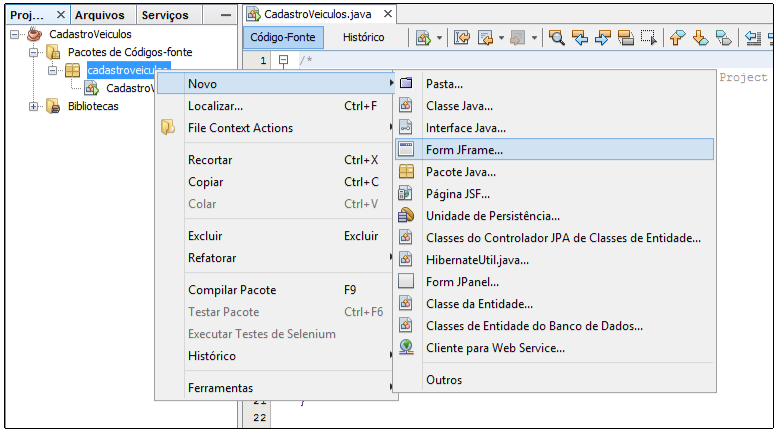
\includegraphics[width=0.6\textheight]{img/gui-criacao-tela}
	\caption{Criação de uma tela (\texttt{JFrame})}
	\label{fig:gui-criacao-tela}
\end{figure}

O NetBeans fornece uma série de ferramentas para suporte à construção de interfaces gráficas. A Figura~\ref{fig:gui-netbeans} mostra a IDE e suas ferramentas. No lado esquerdo, podemos acessar a estrutura do projeto e seus arquivos. Na parte central observamos a tela que está sendo construída. Nela podemos inserir componentes, posicioná-los e configurá-los. Na parte direita (acima) encontramos a paleta de componentes. Através dela é possível selecionar os componentes desejados e arrastá-los até a área de construção da interface. Logo abaixo observa-se as propriedades dos elementos. Basta selecionar um componente inserido na interface e suas propriedades são apresentadas, possibilitando a alteração e ajuste dos seus valores.

\begin{figure}[h]
	\centering
	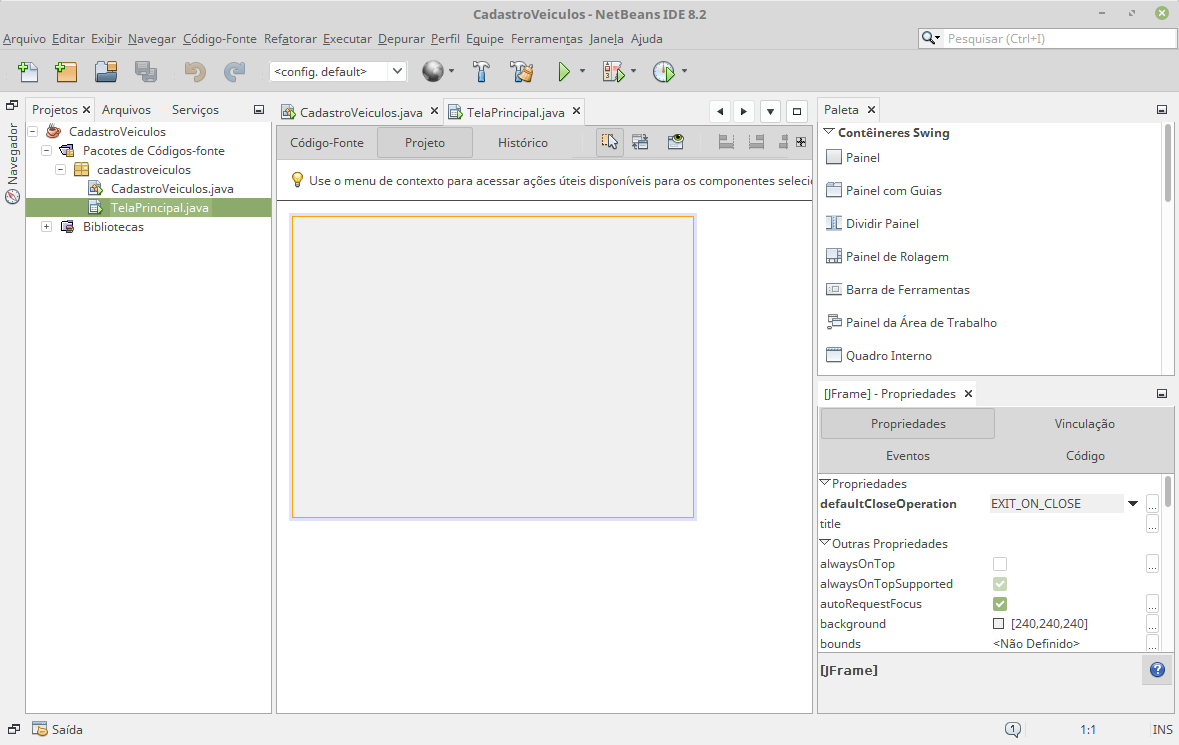
\includegraphics[width=0.6\textheight]{img/gui-netbeans}
	\caption{NetBeans com ferramentas para interfaces gráficas}
	\label{fig:gui-netbeans}
\end{figure}

O componente \texttt{JFrame}, que consiste em uma tela através do qual o usuário interage com o sistema, é criado automaticamente com um método \code{main}, permitindo que a aplicação inicie por ele. O ideal é que uma classe de controle seja responsável por iniciar o sistema e criar as suas telas. Porém, por questões de simplicidade, utilizaremos a \code{TelaPrincipal} como ponto de partida da aplicação. Logo, a classe principal criada no projeto pode ser excluída. A Figura~\ref{fig:gui-estrutura-inicial} mostra a estrutura atual do projeto.

\begin{figure}[h]
	\centering
	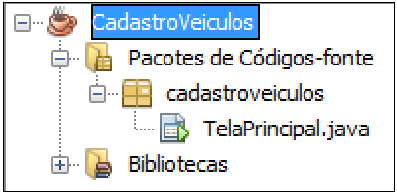
\includegraphics[width=0.4\textheight]{img/gui-estrutura-inicial}
	\caption{Estrutura inicial do projeto}
	\label{fig:gui-estrutura-inicial}
\end{figure}

Logo acima da pré-visualização da interface encontram-se algumas abas (chamadas visões), entre elas \texttt{Código-fonte} e \texttt{Projeto}. Ao selecionar a aba \texttt{Projeto}, as ferramentas de construção visuais são apresentadas. Ao selecionar a aba \texttt{Código-fonte}, o código gerado é apresentado e o programador pode fazer as alterações desejadas e a implementação dos métodos da aplicação.

Abaixo é apresentado o código para a tela inicial criada. Perceba que a classe estende \code{JFrame}. O método \code{main} cria a janela e a torna visível. No construtor, todos os componentes inseridos na tela são inicializados. Nesta classe podemos definir nossas variáveis, como a lista de veículos e os objetos necessários à sua manipulação.

\begin{minted}{java}
public class TelaPrincipal extends javax.swing.JFrame {
	
	public TelaPrincipal() {
		initComponents();
	}
	
	@SuppressWarnings("unchecked") 
	//Generated code
	
	public static void main(String args[]) { 
		java.awt.EventQueue.invokeLater(new Runnable() {
			public void run() { 
				new TelaPrincipal().setVisible(true); 
			}
		});
	}
}    
\end{minted}
    
\section{Barra de menu, eventos e ações}

Utilizando a visão de \texttt{Projeto}, na categoria \texttt{Menus Swing} da paleta de componentes, arraste o elemento \texttt{Barra de Menu} para a janela. Será criado um menu com as opções \texttt{File} e \texttt{Edit}. Clicando com o botão direito sobre estes itens é possível:

\begin{itemize}
	\item Editar o texto que é apresentado em tela.
	\item Alterar o nome da variável (objeto) do componente.
	\item Adicionar itens a esta opção do menu (\texttt{Adicionar da Paleta} > \texttt{Item de Menu}).
	\item Para cada item adicionado, é possível realizar as mesmas ações.
\end{itemize}

Com o uso destas opções, crie configuração do menu apresentada na Figura~\ref{fig:gui-menu}.

\begin{figure}[h]
	\centering
	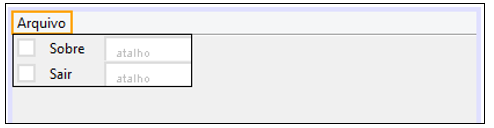
\includegraphics[width=0.4\textheight]{img/gui-menu}
	\caption{Menu para a aplicação \texttt{CadastroVeiculos}}
	\label{fig:gui-menu}
\end{figure}

\textbf{OBS:} é importante definirmos nomes sugestivos a cada objeto que será manipulado, de forma a dar legibilidade ao código. Exemplos: \code{menuArquivo}, \code{menuSobre} e \code{menuSair}.

Execute a aplicação e veja o resultado, que deve ser parecido com o apresentado na Figura~\ref{fig:gui-aplicacao-inicial}. O título da tela (``Cadastro de Veículos'') pode ser definido na propriedade \texttt{title} da janela. Selecionando a janela, suas propriedades são apresentadas na parte direita da interface. Basta, portanto, localizar e alterar a propriedade desejada.

\begin{figure}[h]
	\centering
	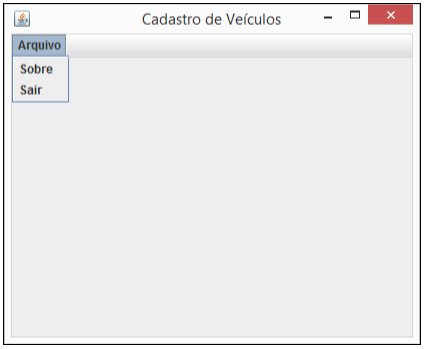
\includegraphics[width=0.4\textheight]{img/gui-aplicacao-inicial}
	\caption{Aplicação inicial com barra de menu}
	\label{fig:gui-aplicacao-inicial}
\end{figure}

do o usuário clicar na opção \texttt{Sobre}, devemos apresentar uma janela com as informações de desenvolvimento da aplicação. Podemos apresentar uma caixa de diálogo (\texttt{JOptionPane}). Logo, basta definirmos a exibição da janela no evento de ação do item de menu correspondente. Ou seja, quando o usuário clica no item, o método (chamado evento) é disparado.

Para isso, clique com o botão direito no item \texttt{Sobre} e selecione as opções \texttt{Eventos} > \texttt{Action} > \texttt{actionPerformed}. A Figura~\ref{fig:gui-action-performed} mostra estas ações. Com isso, o NetBeans criará um método que é invocado sempre que o item de menu for selecionado pelo usuário. Nele, podemos implementar o comportamento desejado.

\begin{figure}[h]
	\centering
	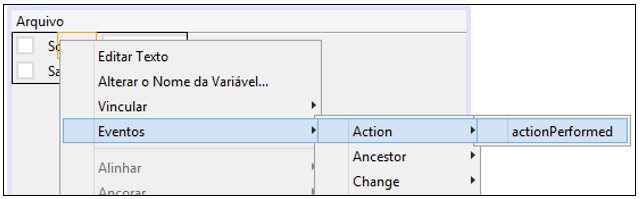
\includegraphics[width=0.4\textheight]{img/gui-action-performed}
	\caption{Definição do evento \texttt{actionPerformed}}
	\label{fig:gui-action-performed}
\end{figure}

O trecho de código abaixo mostra a implementação do método que é disparado no evento de ação do componente \code{menuSobre}. Quando o usuário clicar neste item, será apresentado uma caixa de diálogo com informações do desenvolvimento. Repare que, uma vez que temos uma janela no sistema, podemos defini-la como componente pai da caixa de diálogo. Isso é feito no primeiro argumento do método \code{showMessageDialog}. A Figura~\ref{fig:gui-tela-sobre} mostra o resultado da execução do evento de clique no item de menu \texttt{Sobre}.

\begin{minted}{java}
private void menuSobreActionPerformed(java.awt.event.ActionEvent evt) {
	JOptionPane.showMessageDialog(this,
		"Desenvolvido na disciplina de Programação I - 25PRO1\n"
		+ "Universidade do Estado de Santa Catarina\n"
		+ "Centro de Educação Superior do Alto Vale do Itajaí");
}
\end{minted}

\begin{figure}[h]
	\centering
	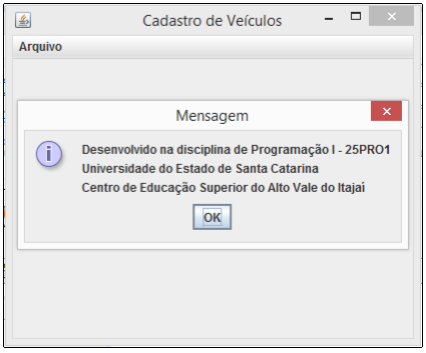
\includegraphics[width=0.4\textheight]{img/gui-tela-sobre}
	\caption{Execução da ação do menu \texttt{Sobre}}
	\label{fig:gui-tela-sobre}
\end{figure}

Faremos o mesmo procedimento para definir o código a ser executado quando o usuário clicar no item \texttt{Sair}. Neste caso, a tarefa é fechar a janela e finalizar a aplicação, mostrando uma mensagem de encerramento. A finalização da aplicação é obtida pelo método \code{dispose}. O trecho de código abaixo mostra sua implementação, enquanto a Figura~\ref{fig:gui-tela-sair} mostra o resultado da sua execução.

\begin{minted}{java}
private void menuSairActionPerformed(java.awt.event.ActionEvent evt) {
	JOptionPane.showMessageDialog(this, "Encerrando a aplicação...");
	dispose();
}
\end{minted}

\begin{figure}[h]
	\centering
	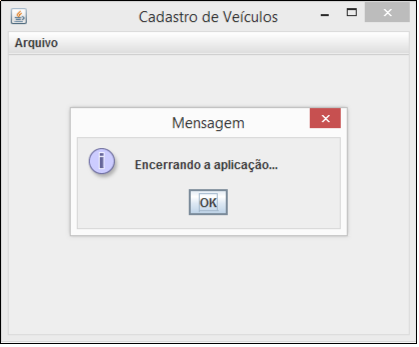
\includegraphics[width=0.4\textheight]{img/gui-tela-sair}
	\caption{Execução da ação do menu \texttt{Sair}}
	\label{fig:tela-sair}
\end{figure}

\section{Entidade Veiculo}

Como a aplicação tem como objetivo o cadastro de veículos, precisamos definir a entidade \code{Veiculo}. Esta classe possui modelo, marca e ano, bem como seus métodos construtores e acessores. A Figura~\ref{fig:gui-veiculo} mostra sua representação UML e o código correspondente é apresentado na sequência.

\begin{figure}[h]
	\centering
	
	\begin{tikzpicture}
	\umlclass{Veiculo}{
		-- modelo: String \\
		-- marca: String \\
		-- ano: int
	}{
		+ métodos construtores \\
		+ métodos acessores
	}	
	\end{tikzpicture}
	
	\caption{Representação UML da classe \code{Veiculo}}
	\label{fig:gui-veiculo}
\end{figure}

\begin{minted}{java}
public class Veiculo {
	private String modelo;
	private String marca;
	private int ano;
	
	//Métodos construtores e acessores
}
\end{minted}


\section{Componentes da tela}

A tela principal deve apresentar um formulário através do qual o usuário poderá cadastrar, consultar, alterar e excluir veículos. Os componentes disponíveis na paleta (alguns deles) são apresentados pela Figura~\ref{fig:gui-paleta}. Para construir a interface desejada, utilizaremos os componentes listados abaixo (entre parêntesis é apresentada a classe que implementa cada componente).

\begin{itemize}
	\item \texttt{Label} (\code{JLabel}): rótulo ou saída de texto na tela.
	\item \texttt{TextField} (\code{JTextField}): campo de entrada de texto.
	\item \texttt{Button} (\code{JButton}): botão de ação.
\end{itemize}

\begin{figure}[h]
	\centering
	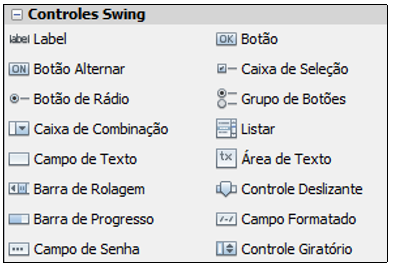
\includegraphics[width=0.4\textheight]{img/gui-paleta}
	\caption{Paleta de componentes \texttt{Swing}}
	\label{fig:gui-paleta}
\end{figure}

A Figura~\ref{fig:gui-formulario} apresenta o formulário formado pelos componentes supracitados. Do lado esquerdo podemos observar os elementos \texttt{Label}, que formam os textos \texttt{Modelo.:}, \texttt{Marca.:} e \texttt{Ano.:}. Os campos de entrada de texto são componentes \texttt{TextField} e os botões são componentes \texttt{Button}. Assim como nos itens de menu, estes objetos devem receber um nome sugestivo e seu texto de apresentação deve ser definido nas propriedades. Posicione cada elemento e define os textos de exibição e nomes sugestivos aos objetos, seguindo a proposta da Figura~\ref{fig:gui-formulario}.

\begin{figure}[h]
	\centering
	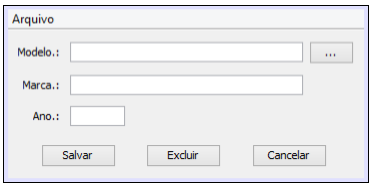
\includegraphics[width=0.4\textheight]{img/gui-formulario}
	\caption{Formulário da tela principal}
	\label{fig:gui-formulario}
\end{figure}

\section{Funcionalidades}

Para implementar as funcionalidades, a classe \code{TelaPrincipal} deverá manter uma lista de veículos (onde os registros serão armazenados) e um objeto da classe \code{Veiculo} (que representará o registro manipulado pelo usuário).

\begin{minted}{java}
public class TelaPrincipal extends javax.swing.JFrame {

	private List<Veiculo> listaVeiculos = new ArrayList<Veiculo>();
	private Veiculo veiculo = new Veiculo();

	//...
}
\end{minted}

\subsection{Salvar registro}
Da mesma forma como é feito com os menus, é possível definir métodos que serão executados quando os botões forem clicados. O processo é o mesmo, definindo um evento do tipo \texttt{actionPerformed}.

O botão \texttt{Salvar} serve para gravar um novo registro na lista, com base nas informações digitadas pelo usuário, ou gravar as alterações feitas pelo usuário em um objeto previamente recuperado da lista. Logo, os passos que devem ser implementados são:

\begin{itemize}
	\item Recuperar os valores digitados pelo usuário no formulário.
	\item Atualizar os atributos do objeto veiculo com os valores recuperados.
	\item Se o objeto não se encontra na lista, é um novo registro e deve ser incluído na mesma. Caso contrário, trata-se de uma alteração e a atualização do objeto já é suficiente.
	\item Instanciar um novo objeto em veiculo, permitindo o cadastro de um novo registro.
	\item Limpar os campos do formulário para que o usuário possa cadastrar um novo registro.
\end{itemize}

O trecho de código abaixo mostra a implementação resultante do método de salvar. Repare que isto é feito no evento de ação do componente \code{btSalvar}. As linhas 2 a 4 recuperam os valores informados pelo usuário na tela. Perceba que é possível acessar os objetos dos componentes, recuperando o valor digitado através do método \code{getText}. As linhas 6 a 8 setam os valores recuperados aos atributos do objeto \code{veiculo}. Nas linhas 10 a 12, se o objeto não se encontra na lista, trata-se de um novo registro e ele deve ser inserido na mesma. Caso contrário, trata-se de uma alteração de um registro existente (pois já encontra-se na lista) e a atualização do objeto já é suficiente. A linha 13 instancia um novo objeto para permitir o cadastro de um novo registro. Finalmente, as linhas 15 a 17 limpam os campos da tela após o cadastro ou alteração.

\begin{minted}{java}
private void btSalvarActionPerformed(java.awt.event.ActionEvent evt) {
	String modelo = edModelo.getText();
	String marca = edMarca.getText();
	int ano = Integer.parseInt(edAno.getText());
	
	veiculo.setModelo(modelo);
	veiculo.setMarca(marca);
	veiculo.setAno(ano);
	
	if(!listaVeiculos.contains(veiculo)) {
		listaVeiculos.add(veiculo);
	}
	veiculo = new Veiculo();
	
	edModelo.setText("");
	edMarca.setText("");
	edAno.setText("");
}
\end{minted}

\subsection{Cancelar preenchimento}

O botão \texttt{Cancelar} deve limpar todos os campos. Caso os valores nos campos sejam referentes a um objeto pesquisado pelo usuário, a referência armazenada em \code{veiculo} deve ser removida e uma nova instância atribuída ao objeto. Isso é feito no método apresentado abaixo, vinculado ao botão \code{btCancelar}.

\begin{minted}{java}
private void btCancelarActionPerformed(java.awt.event.ActionEvent evt) {
	edModelo.setText("");
	edMarca.setText("");
	edAno.setText("");
	veiculo = new Veiculo();
}
\end{minted}

\subsection{Excluir registro}

O botão \texttt{Excluir} remove da lista de veículos um registro pesquisado anteriormente. Como o registro pesquisado se encontra armazenado no objeto \code{veiculo}, basta removê-lo da lista, atribuir uma nova instância a ele e limpar os campos da tela. Isso é feito no método apresentado abaixo, vinculado ao botão \code{btExcluir}.

\begin{minted}{java}
private void btExcluirActionPerformed(java.awt.event.ActionEvent evt) {
	listaVeiculos.remove(veiculo);
	this.veiculo = new Veiculo();

	edModelo.setText("");
	edMarca.setText("");
	edAno.setText("");
}
\end{minted}

\subsection{Pesquisar registro}

O botão \texttt{Pesquisar} permite recuperar um objeto da lista de veículos e preencher os campos do formulário com os valores dos seus atributos. Essa pesquisa é feita com base no valor de modelo informado pelo usuário, por isso o botão se localiza ao lado deste campo.

Caso o veículo seja encontrado, sua referência deve ser armazenada no objeto \code{veiculo} e os campos do formulário são preenchidos com os valores dos seus atributos. Com isso, caso o usuário modifique os valores dos campos e clique em \texttt{Salvar}, o objeto da lista de veículos será atualizado, ao invés de incluído um novo objeto. Caso o usuário clique em \texttt{Excluir}, o objeto será removido da lista. Caso o usuário clique em \texttt{Cancelar}, nada é realizado e os campos e o objeto são ``reiniciados''.

O código vinculado ao evento de ação do botão \texttt{Pesquisar} é apresentado abaixo. Na linha 2, o modelo digitado pelo usuário é recuperado. A lista de veículos é percorrida e, caso encontrado um objeto com o modelo buscado, sua referência é armazenada em \code{veiculo} e seus atributos são inseridos nos campos do formulário (linhas 4 a 11).

\begin{minted}{java}
private void btPesquisarActionPerformed(java.awt.event.ActionEvent evt) {
	String modelo = edModelo.getText();

	for(Veiculo v : listaVeiculos) {
		if(v.getModelo().equals(modelo)) {
			veiculo = v;
			edModelo.setText(veiculo.getModelo());
			edMarca.setText(veiculo.getMarca());
			edAno.setText(String.valueOf(veiculo.getAno()));
			break;
		}
	}
}
\end{minted}

\subsection{Excluir registro}

Uma característica importante do botão \texttt{Excluir} é o fato de ele não fazer sentido quando o usuário está cadastrando um novo veículo. Sua funcionalidade só pode ser executada quando o usuário carregar um veículo previamente cadastrado. Para evitar problemas, podemos desabilitar o botão quando o mesmo não deve ser clicado, impedindo que o usuário execute o método vinculado a ele e deixando claro sua impossibilidade de uso.

Isso pode ser feito feito modificando a propriedade \texttt{enabled} através do método \code{setEnabled(true)} ou \code{setEnabled(false)}, habilitando e desabilitando o componente. O trecho de código abaixo apresenta um exemplo do uso deste método.

\begin{minted}{java}
btExcluir.setEnabled(true);
btExcluir.setEnabled(false);
\end{minted}

O botão \texttt{Excluir} deve ser habilitado nos seguintes casos:

\begin{itemize}
	\item Quando a ação de pesquisa encontra o objeto e o carrega na tela, permitindo ao usuário excluir o veículo, se desejado.
\end{itemize}

O botão \texttt{Excluir} deve ser desabilitado nos seguintes casos:

\begin{itemize}
	\item Quando a ação de salvar é realizada, pois pode se tratar de um objeto carregado da lista, com suas alterações sendo salvas.
	\item Quando a ação de cancelar é realizada, pois pode se tratar de um objeto carregado da lista, onde o usuário está cancelando sua alteração.
	\item Quando a ação de exclusão é realizada, pois ao concluir a exclusão de um registro, uma nova instância é definida e não é possível excluir novamente.
	\item Quando a aplicação inicia, pois o botão deve estar desabilitado por padrão. Isso pode ser feito no construtor da classe, após a inicialização dos seus componentes (trecho de código abaixo).
\end{itemize}

\begin{minted}{java}
public TelaPrincipal() {
	initComponents();
	btExcluir.setEnabled(false);
}
\end{minted}

\section{Outros componentes}

Existem muitos outros componentes swing para a construção de interfaces gráficas interativas. A Figura~\ref{fig:gui-outros-componentes} apresenta a aplicação de componentes de \textit{checkbox}, \textit{radio button}, menu de seleção, campo de senha, área de texto e caixa de seleção.

\begin{figure}[h]
	\centering
	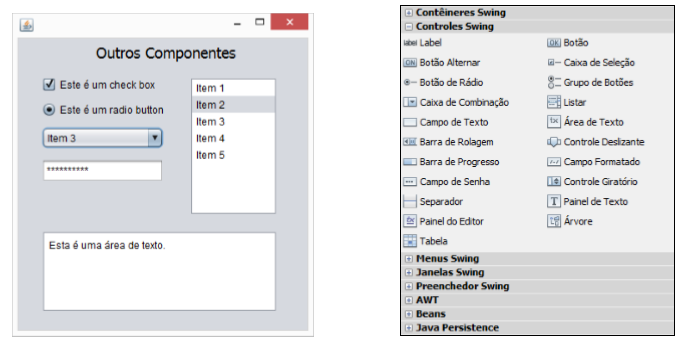
\includegraphics[width=0.4\textheight]{img/gui-outros-componentes}
	\caption{Outros componentes \texttt{swing}}
	\label{fig:gui-outros-componentes}
\end{figure}

Para consultar a documentação dos componentes que deseja utilizar, consulte \url{http://docs.oracle.com/javase/8/docs/api}.
\chapter{Persistência em arquivos}
	
Aplicações precisam de algum mecanismo de persistência de dados, pois informações armazenadas na memória são perdidas sempre que a aplicação é encerrada. A forma mais simples de fazer isso em Java é salvar os dados em arquivos. As operações de leitura e escrita de dados em arquivos são feitas através das bibliotecas de entrada e saída do Java (ou bibliotecas I/O – Input/Output). A Figura~\ref{fig:file-esquema} mostra o esquema geral da biblioteca de entrada e saída que será usada neste capítulo. O programa em Java comunica-se com as classes \code{FileReader} e \code{FileWriter} para as operações de leitura e gravação de dados no arquivo.

\begin{figure}[h]
	\centering
	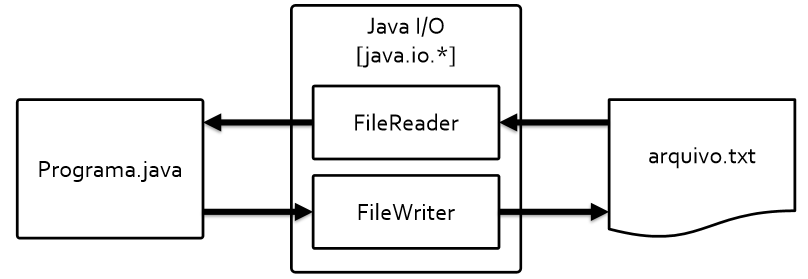
\includegraphics[width=0.4\textheight]{img/file-esquema}
	\caption{Esquema de classes para persistência em arquivos}
	\label{fig:file-esquema}
\end{figure}

\section{Operação de escrita}

A classe \code{FileWriter} fornece os métodos necessários para a escrita de dados em arquivos. Na sua criação, é passado o nome do arquivo e o argumento \code{append}. Se verdadeiro, caso existam informações no arquivo, elas são mantidas e os novos dados são inseridos no final do arquivo. Se falso, caso existam informações no arquivo, elas são apagadas e os novos dados são inseridos no seu lugar.

O trecho de código abaixo mostra o uso da classe \code{FileWriter} para escrita de dados. O método \code{write} recebe como parâmetro o valor e o escreve no arquivo vinculado ao \code{writer} (neste exemplos, \texttt{pessoas.txt}). Repare que é necessário fechar o \code{writer} após o uso, bem como circundar o código com instruções \code{try-catch} para tratar o disparo de exceções no acesso ao arquivo em disco.

\begin{minted}{java}
try {
	FileWriter writer = new FileWriter("pessoas.txt", true);
	writer.write("Este texto será inserido no arquivo");
	writer.write("\n");
	writer.close();
} catch (IOException ex) {
	Logger.getLogger(
		PersistenciaArquivos.class.getName()).log(Level.SEVERE, null, ex);
}
\end{minted}

\section{Operação de leitura}

A classe \code{FileReader} fornece métodos para abertura de arquivos e leitura dos seus dados. Porém, seus métodos permitem apenas a leitura de caracteres. Para ler os dados por linha, utilizaremos um objeto da classe \code{BufferedReader}. Na criação, instanciamos um novo \code{FileReader} passando o nome do arquivo.

O trecho de código mostra a implementação do método de leitura de dados usando as classes supracitadas. O método \code{readLine} faz a leitura de toda a linha e passa para a próxima. Após ler a última linha do arquivo, o método devolve \code{null}. Por isso, enquanto a linha lida for diferente de nulo, a linha é impressa em tela. Após o término, o \code{reader} é fechado. Assim como os métodos de escrita, o código deve ser circundado com as instruções \code{try-catch}.

\begin{minted}{java}
try {
	BufferedReader reader = new BufferedReader(new FileReader("pessoas.txt"));
	String linha;
	while((linha = reader.readLine()) != null) {
		System.out.println(linha);
	}
	reader.close();
} catch (FileNotFoundException ex) {} catch (IOException ex) {}
\end{minted}


\section{Exemplo -- Cadastro de Pessoas}

Considere um sistema para cadastro de pessoas com persistência dos dados em arquivos texto. O sistema deve fornecer as operações de cadastro, exclusão, consulta de uma pessoa pelo seu nome e consulta de todas as pessoas cadastradas.

\subsection{Entidade Pessoa}

O trecho de código abaixo mostra a classe \code{Pessoa}, que define a entidade que será cadastrada e persistida. Repare no método \code{toWriteString} (linhas 8 a 10), que retorna o texto que será usado para armazenar a pessoa no arquivo, com cada atributo separado pelo caracter \texttt{';'}. O método \code{toString}, por sua vez, retorna o texto que deve ser usado para apresentar o objeto em tela.

\begin{minted}{java}
public class Pessoa {
	private String nome;
	private int idade;
	private char sexo;

	//Métodos construtores omitidos

	public String toWriteString() {
		return nome + ";" + idade + ";" + sexo;
	}

	public String toString() {
		String genero;
		if(sexo == 'M') genero = "masculino";
		else genero = "feminino";
		return nome + ", possui " + idade + " anos de idade e é do sexo " + genero + ".";
	}

	//Métodos acessores omitidos
}
\end{minted}

\subsection{Classe para persistência de dados}

O trecho de código abaixo mostra a classe \code{PersistenciaArquivos}, cuja responsabilidade é fornecer métodos para as operações desejadas (cadastro, exclusão e consulta de pessoas). O método \code{inserir} armazena uma pessoa no arquivo. O método \code{ler} recupera uma pessoa do arquivo pelo seu nome, recebido como argumento. O método \code{lerTodasPessoas} devolve uma lista com todas as pessoas armazenadas no arquivo. O método \code{excluir} remove uma pessoa do arquivo pelo seu nome, recebido como argumento.

\begin{minted}{java}
public class PersistenciaArquivos {
	public static void excluir(String nome) {
		//...
	}

	public static List<Pessoa> lerTodasPessoas() {
		//...
	}

	public static Pessoa ler(String nome) {
		//...
	}

	public static void inserir(Pessoa p){
		//...
	}
}
\end{minted}

\subsection{Escrita de uma pessoa}

O método \code{inserir} recebe um objeto da classe \code{Pessoa} e o armazena no arquivo. Seu código é apresentado abaixo. Neste processo, o método armazena no arquivo o conteúdo retornado pelo método \code{toStringFile}. Cada pessoa é escrita em uma linha, portanto ao final de cada pessoa é armazenada uma quebra de linha (\code{\textbackslash n}).

\begin{minted}{java}
public static void inserir(Pessoa p){
	try {
		FileWriter writer = new FileWriter("pessoas.txt", true);
		writer.write(p.toWriteString());
		writer.write("\n");
		writer.close();
	} catch (IOException ex) {
		Logger.getLogger(PersistenciaArquivos.class.getName()).log(
			Level.SEVERE, null, ex);
	}
}
\end{minted}

\subsection{Leitura de uma pessoa}

O código abaixo mostra a implementação do método \code{ler}, que recebe o nome de uma pessoa (\code{String}) e retorna um objeto da classe \code{Pessoa} com a referência buscada, caso encontrado. Caso contrário, o método retorna \code{null}. O arquivo é lido linha por linha, ou seja, enquanto o retorno do método \code{readLine} for diferente de \code{null} (linha 5). Cada linha é dividida pelo caracter separador (\texttt{';'}), de modo a obter o valor de cada atributo da pessoa armazenada no arquivo. Esta operação é feita pelo método \code{split} (linha 6 -- detalhado abaixo). Caso o nome da pessoa seja igual ao nome buscado, a pessoa é recuperada (linha 7). Nas linhas 8 a 13 o objeto \code{Pessoa} é criado e seus atributos são recuperados, para então retorná-lo.

\begin{minted}{java}
public static Pessoa ler(String nome) {
	try {
		BufferedReader reader = new BufferedReader(new FileReader("pessoas.txt"));
		String linha;
		while((linha = reader.readLine()) != null) {
			String[] conteudo = linha.split(";");
			if(conteudo[0].equals(nome)) {
				Pessoa p = new Pessoa();
				p.setNome(conteudo[0]); //nome na [0]
				p.setIdade(Integer.parseInt(conteudo[1])); //idade na [1]
				p.setSexo(conteudo[2].charAt(0)); //sexo [2]
				reader.close();
				return p;
			}
		}
		reader.close();
	} catch (FileNotFoundException ex) {} catch (IOException ex) {}
	return null;
}
\end{minted}

O método \code{split} divide a \code{String} conforme o caracter recebido (no exemplo, é usado o caracter \texttt{';'}). Ele separa cada valor e adiciona em uma posição de um vetor de String, retornando-o. O código abaixo exemplifica o uso do método \code{split}.

\begin{minted}{java}
String texto = "Este texto;está separado;para posterior;recuperação!";
String[] conteudo = texto.split(";");
\end{minted}

\begin{minipage}{\textwidth}
	\textbf{\texttt{Resultado:}}\\
	\texttt{\code{conteudo[0]}    ``Este texto''}\\
	\texttt{\code{conteudo[1]}    ``está separado''}\\
	\texttt{\code{conteudo[2]}    ``para posterior''}\\
	\texttt{\code{conteudo[3]}    ``recuperação!''}\\
\end{minipage}


\subsection{Leitura de todas as pessoas}

O trecho de código a seguir mostra a implementação do método \code{lerTodasPessoas}, que faz a leitura de todos os registros de pessoas armazenados no arquivo, retornando uma lista de objetos da classe \code{Pessoa}. A leitura é igual à de uma pessoa, mas todas as linhas são lidas, atribuídas ao objeto Pessoa e incluídos na lista, que é devolvida ao final do método.

\begin{minted}{java}
public static List<Pessoa> lerTodasPessoas() {
	List<Pessoa> listaPessoas = new ArrayList<Pessoa>();
	try {
		BufferedReader reader = new BufferedReader(new FileReader("pessoas.txt"));
		String linha;
		while((linha = reader.readLine()) != null) {
			String[] conteudo = linha.split(";");
			Pessoa p = new Pessoa();
			p.setNome(conteudo[0]);
			p.setIdade(Integer.parseInt(conteudo[1]));
			p.setSexo(conteudo[2].charAt(0));
			listaPessoas.add(p);
		}
		reader.close();
	} catch (FileNotFoundException ex) {} catch (IOException ex) {}
	return listaPessoas;
}
\end{minted}

\subsection{Exclusão de uma pessoa}

Como não existe um método para excluir uma linha única de um arquivo, a estratégia de exclusão consiste em ler todos os dados, apagar todo o arquivo e reescrever todos os registros novamente, exceto aquele que deve ser excluído. O trecho de código abaixo mostra a implementação do método \code{excluir}. Repare que o método carrega uma lista com todas as pessoas (linha 2) e a percorre. Apenas os dados da pessoa buscada não são inseridos na \code{String} a ser regravada (linhas 6 e 7). Após lidas todas as pessoas, o arquivo é aberto com modo \code{append = false}, que apaga todos os registros previamente armazenados, para então gravar os novos dados.

\begin{minted}{java}
public static void excluir(String nome) {
	List<Pessoa> todasPessoas = lerTodasPessoas();
	String conteudo = "";

	for(Pessoa p : todasPessoas) {
		if(!p.getNome().equals(nome))
			conteudo += p.toWriteString() + "\n";
	}

	try {
		FileWriter writer = new FileWriter("pessoas.txt", false);
		writer.write(conteudo);
		writer.close();
	} catch (IOException ex) {
		Logger.getLogger(PersistenciaArquivos.class.getName()).log(
			Level.SEVERE, null, ex);
	}
}
\end{minted}

\textbf{OBS:} uma estratégia similar pode ser adotada na edição de dados, onde todos os registros são reescritos, atualizando os atributos do registro buscado.

\part{Apêndices}
\appendix
\chapter{Lista de exercícios}
\renewcommand\thechapter{}
\renewcommand\thesection{\arabic{section}}

\section{Revisão sobre Java}

\begin{exercise}[Salario]
Uma empresa decide dar um aumento de 25,5\% aos funcionários cujo salário é inferior a R\$ 2.000,00 e tenha mais de 2 dependentes, 15\% para os que ganham acima ou igual de R\$ 2.000,00 e tenham um dependente e 7,5\% para os que ganham acima de R\$ 3.000,00 e não tenham dependente. Escreva um algoritmo que leia as informações de um funcionário e informe seu salário reajustado conforme regras.
\end{exercise}

\begin{exercise}[Bhaskara]
Escreva um programa para resolver equações do segundo grau. O algoritmo deverá ler os coeficientes A, B e C e resolver a equação conforme instruções abaixo.

$$
x = {-b \pm \sqrt{b^2 - 4ac}} \over {2a}
$$

Identifique os casos onde não existe uma raiz real (interior da raiz quadrada negativo), existe uma única raiz real (interior da raiz quadrada igual a zero) e quando existem duas raízes reais (interior da raiz quadrada maior que zero). Apresente em tela a(s) raiz(es) da função.

\end{exercise}

\begin{exercise}[NumeroPrimo]
Escreva um programa que leia um numero inteiro positivo e diga se ele é um número primo. O programa deverá ser executado para quantos números o usuário desejar. O usuário pode finalizar a execução do algoritmo informando $-1$.
\end{exercise}

\begin{exercise}[MediaTurma]
Na disciplina de programação, são realizadas três provas ao longo do semestre. Escreva um algoritmo que leia as três notas de cada um dos alunos (o número de alunos na disciplina é informado no início da execução do algoritmo). Considerando a média aritmética simples das três notas, o algoritmo deve informar a quantidade de alunos aprovados, de alunos em exame e de alunos reprovados. Para aprovar a disciplina a média deve ser maior ou igual a 7. Uma média maior ou igual a 3 e menor que 7 deixa o aluno em exame, enquanto uma média menor que 3 implica na reprovação do aluno.
\end{exercise}

\begin{exercise}[Calculos]
Crie um programa que leia um valor inteiro positivo. Crie três métodos para realização de cálculos sobre o valor informado. O primeiro método recebe o valor como parâmetro e retorna seu fatorial. O segundo método recebe o valor como parâmetro e calcula a soma de todos os números naturais menores ou iguais ao valor informado. O terceiro método recebe o valor como parâmetro e imprime todos os números ímpares entre o valor informado e 50.
\end{exercise}

\begin{exercise}[BeneficioFuncionarios]
Uma empresa pretende ofertar um benefício aos funcionários carentes. Funcionários com pelo menos 10 anos de serviço e pelo menos 30 anos de idade têm o direito de receber o benefício. O valor pago a eles é calculado em função do salário e da quantidade de dependentes (tabela abaixo). Escreva um algoritmo que leia o tempo de serviço do funcionário, sua idade, seu salário e a quantidade de dependentes. Escreva um método que determina se o funcionário tem direito ao benefício, um segundo método para calcular o valor do benefício e um terceiro método que determina o novo valor do seu salário.

\begin{table}[]
	\centering
	\begin{tabular}{llr}
		\hline
		\textbf{Salário}                       & \textbf{Dependentes} & \textbf{Benefício} \\ \hline
		\multirow{2}{*}{Até R\$ 1.500,00}      & Até 2                & R\$ 500,00         \\
		& Mais que 2           & R\$ 800,00         \\ \hline
		\multirow{2}{*}{Acima de R\$ 1.500,00} & Até 2                & R\$ 300,00         \\
		& Mais que 2           & R\$ 500,00         \\ \hline
	\end{tabular}
\end{table}

\end{exercise}

\begin{exercise}[OperacoesVetores]
Escreva um algoritmo que leia os valores de dois vetores de inteiros de 10 posições. Após a leitura, deverá ser criado um terceiro vetor para armazenar a soma dos elementos. Isto é, o valor da posição 0 do terceiro vetor corresponde à soma dos valores armazenados na posição 0 dos dois primeiros vetores. Neste sentido, crie vetores adicionais para armazenar a subtração, multiplicação e divisão (real) dos dois vetores iniciais.
\end{exercise}

\begin{exercise}[TrocaVetores]
Faça um programa que leia os valores de um vetor de n posições (n deverá ser um número par e será informado no início da execução do algoritmo). Após isso, troque os elementos das primeiras n/2 posições com os elementos das últimas n/2 posições, apresentando o resultado em tela. Finalmente, apresente a soma dos números pares e o produto dos números ímpares armazenados no vetor.
\end{exercise}

\begin{exercise}[OperacoesMatriz]
Escreva um algoritmo que faça a leitura de uma matriz quadrada de tamanho n (o tamanho também deve ser fornecido pelo usuário) com número inteiros. Após a leitura, o algoritmo deverá apresentar a soma dos valores abaixo da diagonal principal, a soma dos valores acima da diagonal principal e o produto dos valores da diagonal principal.
\end{exercise}

\begin{exercise}[GeraMatriz]
Faça um algoritmo que leia uma matriz de ordem NxM com números inteiros e some cada uma das linhas, armazenando o resultado das somas em um vetor. A seguir, multiplique cada elemento da matriz pela soma da linha e mostre a matriz resultante.
\end{exercise}

\begin{exercise}[Palindromo]
Crie um programa que faça a leitura de uma palavra e verifique se a mesma é um palíndromo. Um palíndromo é uma palavra que, quando invertida, não é modificada. Exemplo: REVER.
\end{exercise}

\begin{exercise}[BuscaPalavra]
Escreva um algoritmo que faça a leitura de um texto informado pelo usuário. Após isso, leia uma palavra também informada pelo usuário. O algoritmo deve determinar se a palavra encontra-se no texto informado. Utilize apenas a função charAt(i), da classe String.
\end{exercise}

\clearpage

\section{Conceitos básicos de orientação a objetos}

\begin{exercise}[CadLivro]
Crie um programa que implemente a classe \texttt{Livro}. Esta classe deve conter o título do livro, nome do autor, editora e quantidade de páginas. Adicione um atributo que armazene a página atual (\texttt{paginaAtual}), para apresentação em um dispositivo eletrônico de leitura. Crie um método \texttt{virarPagina}, que incrementa o valor armazenado em \texttt{paginaAtual}. Após isso, crie uma segunda classe chamada \texttt{Main} (classe principal) que conterá o método \texttt{main}. Nesta classe, crie um objeto \texttt{Livro} e preencha seus atributos com valores lidos do usuário. Após isso, chame o método para virar uma página e apresente o objeto (seu estado) em tela. A classe \texttt{Livro} é apresentada abaixo.

\begin{figure}[h]
	\centering
	\begin{tikzpicture}
	\umlclass{Livro}{ 
		-- titulo: String \\
		-- autor: String \\
		-- editora: String \\
		-- numPags: int \\
		-- pagAtual: int = 0
	}{ 
		+ métodos construtores \\
		+ métodos set() e get() \\
		+ virarPagina(): void
	}
	\end{tikzpicture}
\end{figure}

\end{exercise}

\begin{exercise}[ListaLivros]
Usando a classe \texttt{Livro}, criada no exercício anterior, crie uma lista para armazenar diferentes livros. Esta lista pode ser criada usando a coleção \texttt{ArrayList}. Crie um conjunto de objetos, solicite ao usuário o valor dos seus atributos e armazene-os na lista. Após isso, apresente o título e o número de páginas de cada livro armazenado. Utilize uma lista global e diferentes métodos para a criação dos objetos e sua apresentação.
\end{exercise}

\begin{exercise}[ConsultaLivro]
Com base no exercício anterior, crie um método para a consulta de livros. O usuário informa o título do livro desejado, o sistema faz a busca na lista de livros e apresenta seus dados, caso o encontre. Caso contrário, o sistema deve apresentar a mensagem "\textit{Livro não encontrado}".
\end{exercise}

\begin{exercise}[ExcluiLivro]
Com base no exercício anterior, crie um método para exclusão de livros. O usuário informa o título do livro que deseja excluir, o sistema faz a busca do livro e o remove da lista, caso o encontre. Caso contrário, o sistema deve apresentar a mensagem "\textit{Livro não encontrado}".
\end{exercise}	

\begin{exercise}[AlteraLivro]
Com base no exercício anterior, crie um método para alteração de livros. O usuário informa o título do livro que deseja alterar, o sistema faz a busca do livro e, caso o encontre, solicita as novas informações ao usuário, atualizando seus campos. Caso contrário. o sistema deve apresentar a mensagem "\textit{Livro não encontrado}".
\end{exercise}

\begin{exercise}[LivrosCompleto]
Com base nos métodos criados nos exercícios anteriores, crie um programa que apresente ao usuário um menu com todas as opções (cadastro de livro, alteração, exclusão, consulta por título, consulta completa e sair). O usuário pode selecionar as opções desejadas e, ao terminar, seleciona a opção \texttt{sair}, que finaliza a execução do programa.
\end{exercise}

\begin{exercise}[Funcionario]
Crie um programa que implemente a classe \texttt{Funcionario} apresentada abaixo. Na classe principal da aplicação, deverá ser criada uma lista para armazenar os funcionários. Crie um menu que forneça ao usuário as seguintes operações:

\begin{figure}[h]
	\centering
	\begin{tikzpicture}
		\umlclass{Funcionario}{ 
			-- cpf: String \\
			-- nome: String \\
			-- idade: int \\
			-- salario: double \\
			-- tempoServico: int \\
			-- dependentes: int
		}{ 
			+ métodos set() e get() 
		}
	\end{tikzpicture}
\end{figure}

\begin{enumerate}
	\item Incluir funcionário.
	\item Excluir funcionário.
	\item Alterar dados de um funcionário.
	\item Consultar funcionário pelo CPF.
	\item Consultar funcionários por tempo mínimo de serviço.
	\item Consultar o salário médio dos funcionários cadastrados.
	\item Consultar o total de dependentes dos funcionários cadastrados.
\end{enumerate}
\end{exercise}

\begin{exercise}[Farmacia]
	Crie um programa para gerenciamento de produtos de uma farmácia. Serão implementadas duas classes: Medicamento e Cosmetico. Um medicamento possui uma descrição, dosagem, nome do laboratório que o fabrica e seu preço. Um cosmético possui uma descrição, marca, número de lote e preço. Crie as representações dessas classes utilizando UML. No programa, crie métodos para o cadastro de medicamentos e cosméticos, bem como a consulta dos registros cadastrados. Crie um método que liste todas as marcas de cosméticos e a quantidade de cosméticos de cada uma delas. Crie um método para mostrar os medicamentos com preço maior que a média de preços dos cosméticos.
\end{exercise}

\begin{exercise}[Calculadora]
	Desenvolva uma calculadora capaz de resolver três cálculos distintos: raízes de funções quadráticas pela fórmula de Bhaskara, hipotenusa de um triângulo retângulo pelo teorema de Pitágoras e área de trapézio. Crie uma classe para cada cálculo, definindo seus atributos em função dos valores necessários para o cálculo.
\end{exercise}

\clearpage

\section{Associações simples}

\begin{exercise}[EquipeTreinador]
Considere as classes \texttt{Equipe} e \texttt{Treinador}. Uma equipe possui um treinador, e um treinador treina uma equipe. A equipe é composta por um nome (\texttt{String}) e uma categoria (\texttt{String}). O treinador possui um nome (\texttt{String}), número de registro (\texttt{int}) e um salário (\texttt{double}). Implemente estas classes com a respectiva associação (considere a navegabilidade de \texttt{Equipe} para \texttt{Treinador}), crie dois objetos (\texttt{Equipe} e \texttt{Treinador}) lendo seus valores do usuário e associe-os. Após isso, mostre o nome da equipe, sua categoria e o nome do seu treinador (o treinador deve ser acessado a partir da equipe, ou seja, usando a associação).
\end{exercise}

\begin{exercise}[ListaEquipes]
Modifique o exercício anterior e torne o relacionamento bidirecional. Crie uma lista de equipes para armazenar os registros. O usuário poderá cadastrar uma série de equipes com seus respectivos treinadores. Ao final, mostre todas as equipes cadastradas juntamente com o nome do treinador e seu número de registro.
\end{exercise}

\begin{exercise}[Natacao]
Considere um sistema para gerenciamento de provas de natação. O sistema deve controlar as provas e os respectivos recordes, armazenando o registro do atleta que o atingiu. Implemente a estrutura de classes abaixo e métodos para cadastro de atletas, provas e recordes. No cadastro do recorde, o programa deve apresentar as provas e solicitar ao usuário que selecione a opção desejada. Após selecionada a prova, o usuário deverá selecionar o atleta seguindo a mesma lógica anterior. Finalmente, o recorde é cadastrado, substituindo o recorde anterior, quando existente.

\textbf{OBS:} Uma prova não precisa, necessariamente, possuir um recorde vinculado. No entanto, o recorde precisa, necessariamente, possuir um atleta vinculado.
	
\begin{figure}[h]
	\centering
	\begin{tikzpicture}
		\umlclass[x=0]{Atleta}{ 
			-- nome: String \\
			-- idade: int
		}{ 
			+ métodos construtores  \\
			+ métodos set() e get() 
		}
		
		\umlclass[x=5.75]{Recorde}{ 
			-- tempo: double
		}{ 
			+ métodos construtores  \\
			+ métodos set() e get() 
		}
		
		\umlclass[x=11.5]{Prova}{ 
			-- descricao: String \\
			-- distancia: int
		}{ 
			+ métodos construtores  \\
			+ métodos set() e get() 
		}
		
		\umluniassoc[geometry=-|-, mult2=1, pos2=2.7, align2=top] {Recorde}{Atleta}
		
		\umluniassoc[geometry=-|-, mult2=0..1, pos2=2.5, align2=top] {Prova}{Recorde}
	\end{tikzpicture}
\end{figure}
\end{exercise}

\begin{exercise}[Imobiliaria]
Crie uma aplicação para o cadastro e manutenção de imóveis. O diagrama de classes abaixo mostra a estrutura da aplicação. Além dos seus atributos primitivos, um imóvel possui um proprietário, que também é modelado por uma classe. O imóvel também possui uma cidade, que também é modelada por uma classe. Note que o imóvel precisa de um proprietário e de uma cidade para ser cadastrado (dadas as multiplicidades das classes). Crie métodos para inserir registros fixos de proprietários e cidades. Crie um método para o cadastro de imóveis onde o usuário informa os dados do imóvel e seleciona o proprietário e a cidade. Crie métodos para a consulta de imóveis por tipo e consulta de imóveis de uma determinada cidade (os filtros são informados pelo usuário).

\begin{figure}[h]
	\centering
	\begin{tikzpicture}
		\umlclass[x=0]{Proprietario}{ 
			-- nome: String \\
			-- cpf: String \\
			-- rg: String
		}{ 
			+ métodos construtores  \\
			+ métodos set() e get() 
		}
	
		\umlclass[x=5.75]{Imovel}{ 
			-- tipo: int \\
			-- area: double
		}{ 
			+ métodos construtores  \\
			+ métodos set() e get() 
		}
	
		\umlclass[x=11.5]{Cidade}{ 
			-- descricao: String
		}{ 
			+ métodos construtores  \\
			+ métodos set() e get() 
		}
	
		\umluniassoc[geometry=-|-, mult2=1, pos2=2.6, align2=top] {Imovel}{Proprietario}
		
		\umluniassoc[geometry=-|-, mult2=1, pos2=2.3, align2=left] {Imovel}{Cidade}
	\end{tikzpicture}
\end{figure}
\end{exercise}

\begin{exercise}[Filmes]
Considere um sistema para controlar a localização de filmes de uma locadora. Neste sentido, o sistema deve implementar a classe \texttt{Estante} (\texttt{numSala}, \texttt{numCorredor}) e \texttt{Filme} (\texttt{titulo}, \texttt{sinopse} e \texttt{duracao}). Um filme estará em uma estante, e uma estante pode conter zero ou muitos filmes. Implemente estas duas classes (com navegabilidade de \texttt{Filme} para \texttt{Estante}), solicite ao usuário as informações de uma estante com três filmes e de uma segunda estante com dois filmes. Faça a associação dos objetos e apresente-os em tela.
\end{exercise}

\begin{exercise}[ListaFilmes]
Modifique as classes do exercício anterior e inverta a navegabilidade da associação. Crie uma lista para armazenar as estantes e solicite ao usuário o cadastro de várias estantes com seus filmes. Ao final, mostre todas as estantes armazenadas na lista, juntamente com o título dos filmes da mesma.
\end{exercise}

\begin{exercise}[Livros]
Crie uma aplicação para o cadastro e manutenção de livros. O diagrama de classes abaixo mostra a estrutura da aplicação. Crie métodos para criar conjuntos de editoras e de gêneros, armazenando os registros em listas. Crie um menu onde o usuário pode escolher as opções de cadastrar, excluir e consultar livros. No cadastro, o usuário deve selecionar uma editora e um gênero para vincular ao livro. Na consulta todas as informações do livro, editora e gênero deverão ser apresentadas.

\begin{figure}[h]
	\centering
	\begin{tikzpicture}
		\umlclass[x=0]{Editora}{ 
			-- nome: String \\
			-- cidade: String
		}{ 
			+ métodos construtores  \\
			+ métodos set() e get() 
		}
		
		\umlclass[x=5.75]{Livro}{ 
			-- titulo: String \\
			-- pags: int \\
			-- ano: int
		}{ 
			+ métodos construtores  \\
			+ métodos set() e get() 
		}
		
		\umlclass[x=11.5]{Genero}{ 
			-- descricao: String
		}{ 
			+ métodos construtores  \\
			+ métodos set() e get() 
		}
		
		\umlassoc[geometry=-|-, mult1=1, pos1=0.3, mult2=0..$*$, pos2=2.55] {Editora}{Livro}
		
		\umluniassoc[geometry=-|-, mult1=0..$*$, pos1=0.45, mult2=1, pos2=2.5, align2=left] {Livro}{Genero}
	\end{tikzpicture}
\end{figure}
\end{exercise}

\begin{exercise}[Artigos]
Crie uma aplicação para o cadastro de artigos científicos. Cada artigo é publicado em uma revista e cada revista pertence a uma instituição. A aplicação deverá permitir o cadastro de instituições, revistas e artigos, bem como a consulta de todos os artigos cadastrados.

\begin{figure}[h]
	\centering
	\begin{tikzpicture}
		\umlclass[x=0]{Instituicao}{ 
			-- nome: String \\
			-- cidade: String
		}{ 
			+ métodos construtores  \\
			+ métodos set() e get() 
		}
		
		\umlclass[x=5.75]{Revista}{ 
			-- nome: String \\
			-- edicao: int \\
			-- ano: int
		}{ 
			+ métodos construtores  \\
			+ métodos set() e get() 
		}
		
		\umlclass[x=11.5]{Artigo}{ 
			-- titulo: String \\
			-- resumo: String
		}{ 
			+ métodos construtores  \\
			+ métodos set() e get() 
		}
		
		\umluniassoc[geometry=-|-, mult1=1, pos1=0.3, mult2=0..$*$, pos2=2.55] {Instituicao}{Revista}
		
		\umluniassoc[geometry=-|-, mult1=1, pos1=0.3, mult2=0..$*$, pos2=2.55] {Revista}{Artigo}
	\end{tikzpicture}
\end{figure}
\end{exercise}

\clearpage

\section{Agregação e composição}

\begin{exercise}[RadarSensor]
Considere as entidades \texttt{Radar} e \texttt{SensorVelocidade}. Um radar possui um sensor de velocidade, que o informa da velocidade do veículo. O sensor de velocidade existe mesmo fora do relacionamento com o radar e pode estar relacionado a dois ou mais radares ao mesmo tempo. Logo, as duas entidades formam um relacionamento de agregação, conforme apresentado abaixo. Escreva o código para estas classes e implemente o método \texttt{List<Radar> radaresPrecisaoMinima(List<Radar> radares, double precisao)}. Este método recebe uma lista de radares e um valor de precisão, e deve retornar uma lista com os radares encontrados que possuem a precisão mínima exigida.

\begin{figure}[h]
	\centering
	
	\begin{tikzpicture}
	\umlclass{Radar}{
		-- velocidadeMaxima: double
	}{
		+ métodos construtores \\
		+ métodos acessores
	}
	
	\umlclass[x=8]{SensorVelocidade}{
		-- precisao: double
	}{
		+ métodos construtores \\
		+ métodos acessores
	}
	
	\umlaggreg[geometry=-|-, mult2=1, pos=2.9, align2=top]{Radar}{SensorVelocidade}
	\end{tikzpicture}
\end{figure}
\end{exercise}

\begin{exercise}[TurmaAluno]
Considere as entidades \texttt{Turma} e \texttt{Aluno}. Os alunos são parte de uma turma, que é a entidade todo. Os alunos existem independente do relcionamento com a turma e um aluno pode pertencer a duas turmas simultaneamente. Logo, temos um relacionamento de agregação (veja diagrama abaixo). Escreva o código das classes e implemente o método \texttt{List<Turma> turmasDoAluno(List<Turma> turmas, String nomeAluno)}, que recebe uma lista de turmas e o nome de um aluno, retornando uma lista com as turmas das quais o aluno faz parte.

\begin{figure}[h]
	\centering
	
	\begin{tikzpicture}
	\umlclass{Turma}{
		-- ano: int \\
		-- semestre: int
	}{
		+ métodos construtores \\
		+ métodos acessores
	}
	
	\umlclass[x=8]{Aluno}{
		-- matricula: String \\
		-- nome: String
	}{
		+ métodos construtores \\
		+ métodos acessores
	}
	
	\umlaggreg[geometry=-|-, mult2=*, pos=2.9, align2=top]{Turma}{Aluno}
	\end{tikzpicture}
	\end{figure}
\end{exercise}

\begin{exercise}[Compras]
Considere um sistema para gerenciar compras feitas pela Internet. Cada compra possui o número da sua nota fiscal e agrega os produtos adquiridos, os quais possuem uma descrição e um valor. O diagrama de classes abaixo apresenta a estrutura dessas entidades. Implemente a estrutura de classes proposta e as funcionalidades de cadastrar uma compra, cadastrar os produtos da compra e listar o valor total de uma compra pelo número da sua nota fiscal.

\textbf{OBS:} Mantenha uma lista de produtos na aplicação. Ao cadastrar um novo produto (sua descrição), a aplicação deverá verificar se este produto já está cadastrado. Neste caso, o produto já existente é vinculado à compra.

\begin{figure}[h]
	\centering
	\begin{tikzpicture}
		\umlclass[x=0]{Compra}{ 
			-- numNota: int
		}{ 
			+ métodos construtores  \\
			+ métodos set() e get() 
		}
		
		\umlclass[x=6]{Produto}{ 
			-- descricao: String \\
			-- valor: double
		}{ 
			+ métodos construtores  \\
			+ métodos set() e get() 
		}
		
		\umlaggreg[geometry=-|-, mult2=$*$, pos2=2.8]{Compra}{Produto}
	\end{tikzpicture}
\end{figure}
\end{exercise}

\begin{exercise}[ComputadorProcessador]
Considere as entidades \texttt{Computador} e \texttt{Processador}. Um computador possui um único processador. O processador fica localizado dentro do computador e, portanto, não existe fora do relacionamento com o computador e não pode estar relacionado com dois ou mais computadores ao mesmo tempo (regras para definição de uma composição). Implemente as classes supracitadas e o método \texttt{mostraProcessadores(List<Computador> computadores)}. Com base na lista de computadores recebida, o método deve mostrar os processadores com mais de um núcleo.

\begin{figure}[h]
	\centering
	
	\begin{tikzpicture}
	\umlclass{Computador}{
	}{
		+ métodos construtores \\
		+ métodos acessores
	}
	
	\umlclass[x=8]{Processador}{
		-- nucleos: int \\
		-- potencia: double
	}{
		+ métodos construtores \\
		+ métodos acessores
	}
	
	\umlcompo[geometry=-|-, mult2=1, pos=2.9, align2=top]{Computador}{Processador}
	\end{tikzpicture}
\end{figure}
\end{exercise}

\begin{exercise}[LivroCapitulos]
Considere as entidades \code{Livro} e \code{Capitulo}. Um livro é composto por vários capítulos. O capítulo é parte de um livro e, portanto, não existe fora do relacionamento. Além disso, um capítulo não deve fazer parte de dois livros ao mesmo tempo. Logo, trata-se de uma composição. Apresente o código das classes supracitadas e a implementação do método \texttt{mostraCapitulos(Livro livro, String palavra)}, que recebe como argumento um livro e mostra os capítulos cujo título contenha a palavra buscada.

\begin{figure}[h]
	\centering
	
	\begin{tikzpicture}
	\umlclass{Livro}{
	}{
		+ métodos construtores \\
		+ métodos acessores
	}
	
	\umlclass[x=8]{Capitulo}{
		-- numero: int \\
		-- titulo: String
	}{
		+ métodos construtores \\
		+ métodos acessores
	}
	
	\umlcompo[geometry=-|-, mult2=*, pos=2.9, align2=top]{Livro}{Capitulo}
	\end{tikzpicture}
	\end{figure}
\end{exercise}

\begin{exercise}[TecladoTecla]
Desenvolva uma aplicação para o armazenamento de teclados de diferentes países. Cada teclado é composto por um conjunto de teclas (diagrama de classes abaixo), as quais são identificadas pelo caracter que possuem. O usuário poderá incluir um novo teclado, juntamente com as suas teclas, bem como listar os teclados (e suas teclas) já cadastrados. Além disso, o usuário poderá informar uma palavra e o sistema deverá informar quais teclados são capazes de escrever a referida palavra (com base nas suas teclas).

\textbf{OBS:} A aplicação não deve manter uma lista de teclas, pois uma tecla só existe em função de um teclado (conceito de composição).

\begin{figure}[h]
	\centering
	\begin{tikzpicture}
		\umlclass[x=0]{Teclado}{ 
			-- pais: String
		}{ 
			+ métodos construtores  \\
			+ métodos set() e get() 
		}
		
		\umlclass[x=6]{Tecla}{ 
			-- valor: char
		}{ 
			+ métodos construtores  \\
			+ métodos set() e get() 
		}
	
		\umlcompo[geometry=-|-, mult2=$*$, pos2=2.8]{Teclado}{Tecla}
	\end{tikzpicture}
\end{figure}
\end{exercise}

\begin{exercise}[GestaoEmpresas]
Crie uma aplicação para a gestão das empresas de um grupo. O diagrama de classes abaixo apresenta a estrutura das classes envolvidas. Uma empresa é composta por departamentos, os quais possuem funcionários. Um funcionário pode trabalhar em mais de um departamento ao mesmo tempo. Crie uma lista de empresas e uma lista de funcionários fixos. Implemente as opções de cadastro de departamento das empresas e a vinculação de funcionários aos seus departamentos.

\begin{figure}[h]
	\centering
	\begin{tikzpicture}
		\umlclass[x=0]{Empresa}{ 
			-- nome: String \\
			-- cnpj: String
		}{ 
			+ métodos construtores  \\
			+ métodos set() e get() 
		}
	
		\umlclass[x=5.75]{Departamento}{ 
			-- nome: String \\
			-- andar: int
		}{ 
			+ métodos construtores  \\
			+ métodos set() e get() 
		}

		\umlclass[x=11.5]{Funcionario}{ 
			-- nome: String \\
			-- matricula: String
		}{ 
			+ métodos construtores  \\
			+ métodos set() e get() 
		}
		
		\umlcompo[geometry=-|-, mult2=$*$, pos2=2.8] {Empresa}{Departamento}
		
		\umlaggreg[geometry=-|-, mult2=$*$, pos2=2.8] {Departamento}{Funcionario}
	\end{tikzpicture}
\end{figure}
\end{exercise}

\clearpage

\section{Dependência}

\begin{exercise}[Calculadora]
Desenvolva uma calculadora na qual o usuário informe, através de um campo de texto, a expressão matemática que deseja calcular. Considere expressões matemáticas simples, com dois valores e um operador aritmético simples (adição, subtração, multiplicação e divisão). Exemplos: ``$5 + 3$''; ``$6 - 2$''; ``$14 * 3$''; ``$15 / 3$''. Após informada a expressão, o sistema deve analisar a entrada, realizar o cálculo correspondente e informar o resultado. O diagrama abaixo mostra a estrutura de classes para este exemplo. A classe \texttt{Aplicacao} faz a leitura dos dados e a apresentação dos resultados. A classe \texttt{Operacoes} é responsável por implementar as operações aritméticas suportadas e é utilizada pela classe \texttt{Aplicacao} por meio de uma dependência.

\begin{figure}[h]
	\centering
	\begin{tikzpicture}
		\umlemptyclass[x=0]{Aplicacao}
	
		\umlclass[x=8]{Operacoes}{
		}{
			+ adicao(double, double): double \\
			+ subtracao(double, double): double \\
			+ multiplicacao(double, double): double \\
			+ divisao(double, double): double
		}
		
		\umlimport{Aplicacao}{Operacoes}
	\end{tikzpicture}
\end{figure}

\end{exercise}

\begin{exercise}[RelatorioPessoas]
Crie um programa para a geração de relatórios de pessoas. Na classe Aplicacao, crie uma lista de pessoas com um conjunto inicial de registros. Um relatório recebe a lista de todas as pessoas cadastradas e devolve a lista filtrada de pessoas, a qual deve ser impressa em tela. O filtro pode ser feito por idade mínima e máxima e por sexo, sendo implementado por uma classe específica. O diagrama abaixo apresenta a estrutura de classes.

\begin{figure}[h]
	\centering
	\begin{tikzpicture}
		\umlclass[x=0]{Pessoa}{ 
			-- nome: String \\
			-- idade: int \\
			-- sexo: char
		}{
		}
		
		\umlclass[x=8]{Relatorio}{ 
		}{
			+ pesquisa(List<Pessoa>, Filtro): List<Pessoa>
		}
		
		\umlclass[x=8,y=-4]{Filtro}{ 
			-- idadeMinima: int \\
			-- idadeMaxima: int \\
			-- sexo: char
		}{
		}
		
		\umlimport{Relatorio}{Pessoa}
		
		\umlimport{Relatorio}{Filtro}
	\end{tikzpicture}
\end{figure}

\end{exercise}

\begin{exercise}[EnvioFormulario]
Desenvolva um programa que leia do usuário os campos de entrada de um formulário e faça o envio destes dados (considere como envio a simples impressão dos dados em tela). O envio é feito por uma classe específica, da qual o formulário depende. O método de envio recebe um vetor de String com todos os dados e os imprime em tela. A estrutura de classes é apresentada abaixo.

\begin{figure}[h]
	\centering
	\begin{tikzpicture}
		\umlclass[x=0]{Formulario}{ 
			-- nome: String \\
			-- email: String \\
			-- mensagem: String
		}{ 
			+ enviar(Sender): void
		}
		
		\umlclass[x=6]{Sender}{ 
		}{ 
			+ enviar(String[]): void 
		}
		
		\umlimport{Formulario}{Sender}
	\end{tikzpicture}
\end{figure}

\end{exercise}

\clearpage

\section{Herança e polimorfismo}

\begin{exercise}[ContasBancarias]
Considere um sistema que armazene contas bancárias. Uma conta possui o número de sua agência, número da conta e o saldo disponível. Além disso, esta entidade deve implementar um método de depósito que recebe uma quantia e adiciona ao seu saldo, bem como um método de saque que subtrai a quantia recebida do seu saldo, quando suficiente. Uma conta pode ser do tipo conta corrente ou conta poupança. A conta corrente possui um limite de crédito que pode ser utilizado quando o saldo não for suficiente para um saque. Isto é, o saldo pode ficar negativo até o limite de crédito da conta. Já a conta poupança possui uma taxa de juros que determina o rendimento mensal da mesma. Implemente a estrutura de classes descrita acima utilizando o conceito de herança. Implemente ainda uma classe Aplicacao que realiza as seguintes operações:

\begin{enumerate}[a)]
	\item Armazena uma lista de contas (que podem ser tanto contas correntes quanto poupanças).
	\item Método que cria registros aleatórios de contas e os armazena na lista.
	\item Método para sacar um valor determinado de todas as contas.
	\item Método que recebe duas contas e um valor e faz a transferência da primeira para a segunda conta.
	\item Método que atualiza o saldo das poupanças, adicionando o rendimento de acordo com sua taxa de juros.
\end{enumerate}

\end{exercise}

\begin{exercise}[FigurasGeometricas]
Crie um sistema para armazenamento de figuras geométricas. Implemente a estrutura de classes abaixo, onde todas as figuras possuem uma cor. Todas elas devem implementar um método para cálculo da sua área e um método para cálculo do seu perímetro. Cada classe deve implementar os atributos necessários para executar estes cálculos. Crie uma classe Aplicacao que implemente um método que, dada uma lista de figuras geométricas, determine a área total de todas as figuras. Além disso, crie um método que, dada uma lista de figuras geométricas, apresente a cor da figura de menor perímetro.

\begin{figure}[h]
	\centering
	\begin{tikzpicture}
		\umlclass[x=4,y=3]{Figura}{}{}
		\umlclass[x=0]{Retangulo}{}{}
		\umlclass[x=4]{Triangulo}{}{}
		\umlclass[x=8]{Circulo}{}{}
		
		\umlinherit[geometry=|-]{Retangulo}{Figura}
		\umlinherit{Triangulo}{Figura}
		\umlinherit[geometry=|-]{Circulo}{Figura}
	\end{tikzpicture}
\end{figure}

\end{exercise}

\begin{exercise}[OperacoesCores]
Utilizando as classes desenvolvidas no exercício anterior, crie uma classe Desenho, composta por figuras geométricas (composição). Crie um método (na classe Aplicacao) que receba um desenho e uma cor e mostre a área total da cor no desenho. Crie um segundo método que receba um desenho e mostre as cores que o compõem e a respectiva área que cada cor ocupa no desenho. Finalmente, crie um terceiro método que receba uma lista de desenhos e uma cor e apresente os desenhos que não possuem a referida cor.
\end{exercise}

\begin{exercise}[Loja]
Considere uma loja que vende equipamentos eletrônicos e roupas. Desenvolva um sistema para o gerenciamento dos produtos da loja. Cada produto mantém seu nome e seu valor. Eletrônicos possuem uma voltagem (110 ou 220) e itens do vestuário possuem um tamanho (P, M ou G). Cada produto possui um método para cálculo do número de parcelas, que por padrão é igual a 4x. No caso dos eletrônicos, produtos acima de R\$ 1000,00 podem ser parcelados em 10x. No caso de roupas, mais duas parcelas podem ser adicionadas ao parcelamento padrão, caso a roupa custe mais que R\$ 200,00. Além disso, os produtos implementam um método que calcula o desconto a ser concedido na venda. Por padrão, é concedido 5\% de desconto, valor que aumenta para 10\% nos eletrônicos. No caso das roupas, um desconto adicional de R\$ 15,00 é dado nas vendas. O sistema deve armazenar em uma lista única todos os produtos do estoque. Com base nisso, implemente os seguintes métodos:

\begin{enumerate}[a)]
\item Cadastro de produtos;
\item Venda de produtos (usuário seleciona um produto da lista e o sistema calcula o valor final e número de parcelas);
\item Método que mostra todos os produtos da lista com desconto superior a R\$ 80,00;
\item Método que mostra todos os produtos da lista que podem ser parcelados em mais de 5x;
\item Método que apresente, para todos os produtos do estoque, seu valor de venda com e sem desconto. Ao final, o método deve mostrar os valores totais caso todos os produtos fossem vendidos com e sem desconto.
\end{enumerate}

\begin{figure}[h]
	\centering
	\begin{tikzpicture}
	\umlclass[x=3,y=4]{Produto}{
		-- descricao: String \\
		-- valor: double
	}{
		+ calculaParcelas(): int \\
		+ caculaDesconto(): double
	}
	
	\umlclass[x=0]{Eletronico}{
		-- voltagem: int
	}{
		+ calculaParcelas(): int \\
		+ caculaDesconto(): double
	}
	
	\umlclass[x=6]{Vestuario}{
		-- tamanho: char	
	}{
		+ calculaParcelas(): int \\
		+ caculaDesconto(): double
	}
	
	\umlinherit[geometry=|-]{Eletronico}{Produto}
	\umlinherit[geometry=|-]{Vestuario}{Produto}
	\end{tikzpicture}
\end{figure}
	
\end{exercise}

\addcontentsline{toc}{chapter}{Referências Bibliográficas}
\nocite{*}
\bibliographystyle{apalike}
\bibliography{referencias}

\end{document}